% Document type, global settings, and packages

\documentclass[12pt]{report}   %12 point font for Times New Roman
\usepackage{subcaption}
\usepackage{fixltx2e}
\usepackage{stmaryrd}

\usepackage{graphicx}  %for images and plots
\usepackage{xcolor}  
\usepackage[letterpaper, left=1in, right=1in, top=1in, bottom=1in]{geometry}
\usepackage{setspace}  %use this package to set linespacing as desired
\usepackage{times}  %set Times New Roman as the font
\usepackage[explicit]{titlesec}  %title control and formatting
\usepackage[titles]{tocloft}  %table of contents control and formatting
%\usepackage[backend=bibtex, sorting=none, bibstyle=ieee, style=authoryear]{biblatex}  %reference manager
%\usepackage{biblatex}   % omit 'round' option if you prefer square brackets
%\usepackage[round]{natbib}   % omit 'round' option if you prefer square brackets
\usepackage[round]{natbib}
\usepackage[bookmarks=true, hidelinks,colorlinks=true,linkcolor=blue,allcolors=blue]{hyperref}
\def\Snospace~{\S{}}
\renewcommand*\sectionautorefname{\Snospace}
%\renewcommand{\sectionautorefname}{\S}
\usepackage{appendix}  %for appendices
\usepackage{rotating}  %for rotated, landscape images
%\usepackage{ulem}  %for underlined section titles
\usepackage[normalem]{ulem}
\usepackage{textcomp} % for text symbols such as copyright etc. 
\usepackage{indentfirst} % To indent the first line of every paragraph
\usepackage{booktabs,array,arydshln} %for better table formatting. 
\usepackage{amsmath} %for formula formatting
\usepackage[T1]{fontenc} % improved font encoding
\usepackage[utf8]{inputenc} % for better handling of non-ASCII characters
%\usepackage{newtxtext} % font choice
\usepackage{newtxmath} 
%\usepackage{lmodern} % font choice 

\usepackage{accents}
\usepackage{multirow}

\usepackage{tikz}
\usetikzlibrary{shapes}
\usetikzlibrary{arrows}
\usetikzlibrary{positioning}
\usetikzlibrary{calc}
\usepackage{placeins}

\usepackage{wrapfig}

\definecolor{salsentemb}{HTML}{08E8DE}
\definecolor{sentemb}{HTML}{1974D2}
\definecolor{decsentemb}{HTML}{7FDAFF}
\definecolor{encemb}{HTML}{FFAA1D}
\definecolor{rencemb}{HTML}{FFAA1D}
\definecolor{lencemb}{HTML}{CC7700}

\definecolor{rdecemb}{HTML}{EFEC43}
\definecolor{ldecemb}{HTML}{BCB910}
\definecolor{decemb}{HTML}{FF007F}
\definecolor{ctxemb}{HTML}{66FF00}
\definecolor{encctxemb}{HTML}{B10058}
\definecolor{decctxemb}{HTML}{FFF34B}
\definecolor{sal}{HTML}{F79C6F}
\definecolor{doc}{HTML}{9B0A16}
\definecolor{sum}{HTML}{330066}
\definecolor{factor}{HTML}{EBE029}
\usepackage[linesnumbered,ruled,vlined]{algorithm2e}
\usepackage{cancel}
\usepackage{tablefootnote}
\usepackage{dsfont}
\usepackage{tcolorbox}

\usepackage[autostyle]{csquotes}
\usepackage{lscape}


\bibliographystyle{plainnat}


%\bibliographystyle{plainnat}

% Bibliography
%Add your bibliography file here
%\bibliography{references}

% prevent certain fields in references from printing in bibliography
%?\AtEveryBibitem{\clearfield{issn}}
%?\AtEveryBibitem{\clearlist{issn}}
%?
%?\AtEveryBibitem{\clearfield{language}}
%?\AtEveryBibitem{\clearlist{language}}
%?
%?\AtEveryBibitem{\clearfield{doi}}
%?\AtEveryBibitem{\clearlist{doi}}
%?
%?\AtEveryBibitem{\clearfield{url}}
%?\AtEveryBibitem{\clearlist{url}}
%?
%?\AtEveryBibitem{%
%?  \ifentrytype{online}
%?    {}
%?    {\clearfield{urlyear}\clearfield{urlmonth}\clearfield{urlday}}}
%?

%\renewbibmacro*{title}{%
%  \ifboolexpr{
%    test {\iffieldundef{title}}
%    and
%    test {\iffieldundef{subtitle}}
%  }
%    {}
%    {\printtext{%
%     \printtext[titlecase]{\usefield{\uline}{title}}%
%     \setunit{\subtitlepunct}%
%     \printfield[titlecase]{subtitle}}%
%     \newunit}%
%  \printfield{titleaddon}}

% Start of Dissertatio Document



\makeatletter
\newcommand{\specialterms}[1]{%
  \@for\next:=#1\do
    {\@namedef{specialterm@\detokenize\expandafter{\next}}{}}%
}
\newcommand\term[1]{%
  \@ifundefined{specialterm@\detokenize{#1}}
    {#1}{\emph{#1}\global\expandafter\let\csname specialterm@\detokenize{#1}\endcsname\relax}%
}
\makeatother


\specialterms{faithful,controllable,machine learning}

\newcommand{\latin}[1]{\textit{#1}}

\newcommand{\abstractive}{abstractive}
\newcommand{\alignmenttraining}{alignment training}
\newcommand{\ancestralsampling}{ancestral sampling}
\newcommand{\Ancestralsampling}{Ancestral sampling}
\newcommand{\attribute}{attribute}
\newcommand{\attributes}{attributes}
\newcommand{\attributevalue}{attribute-value}
\newcommand{\attributevalues}{attribute-values}
\newcommand{\Automaticsummarization}{Automatic summarization}
\newcommand{\autoregressive}{autoregressive}
\newcommand{\bidirectional}{bidirectional}
\newcommand{\contentselection}{content selection}
\newcommand{\controllable}{controllable}
\newcommand{\control}{control}
\newcommand{\controllablegeneration}{controllable generation}
\newcommand{\Controllablegeneration}{Controllable generation}
\newcommand{\ConvolutionalNeuralNetwork}{Convolutional Neural Network}
\newcommand{\convolutionalneuralnetwork}{convolutional neural network}
\newcommand{\Dialogueacts}{Dialogue acts}
\newcommand{\dialogueact}{dialogue act}
\newcommand{\dataandtexttotext}{data- and text-to-text}
\newcommand{\datatotext}{data-to-text}
\newcommand{\DeepLearning}{Deep Learning}
\newcommand{\Deeplearning}{Deep learning}
\newcommand{\deeplearning}{deep learning}
\newcommand{\elementwise}{element-wise}
\newcommand{\encoder}{encoder}
\newcommand{\extractive}{extractive}
\newcommand{\extract}{extract}
\newcommand{\extractor}{extractor}
\newcommand{\faithful}{faithful}
\newcommand{\faithfulness}{faithfulness}
\newcommand{\faithfulgeneration}{faithful generation}
\newcommand{\featurebased}{feature-based}
\newcommand{\FeedForward}{Feed-Forward}
\newcommand{\feedforward}{feed-forward}
\newcommand{\gatedrecurrentunit}{gated recurrent unit}
\newcommand{\kernelwidth}{kernel width}
\newcommand{\ignore}{ignore}
\newcommand{\languagegeneration}{language generation}
\newcommand{\linearizationstrategies}{linearization strategies}
\newcommand{\linearizationstrategy}{linearization strategy}
\newcommand{\linearize}{linearize}
\newcommand{\machinelearning}{machine learning}
\newcommand{\machinetranslation}{machine translation}
\newcommand{\meaningrepresentation}{meaning representation}
\newcommand{\meaningrepresentations}{meaning representations}
\newcommand{\MeaningRepresentation}{Meaning Representation}
\newcommand{\MeaningRepresentations}{Meaning Representations}
\newcommand{\naturallanguagegeneration}{natural language generation}
\newcommand{\naturallanguageprocessing}{natural language processing}
\newcommand{\naturallanguageunderstanding}{natural language understanding}
\newcommand{\nonautoregressive}{non-autoregressive}
\newcommand{\nugget}{nugget}
\newcommand{\partofspeech}{part of speech}

\newcommand{\RecurrentNeuralNetwork}{Recurrent Neural Network}
\newcommand{\recurrentneuralnetwork}{recurrent neural network}
\newcommand{\rouge}{\textsc{Rouge}}
\newcommand{\meteor}{\textsc{Meteor}}
\newcommand{\Salienceestimation}{Salience estimation}
\newcommand{\salienceestimation}{salience estimation}
\newcommand{\Salience}{Salience}
\newcommand{\salience}{salience}
\newcommand{\saliencefactors}{salience factors}
\newcommand{\saliencefactor}{salience factor}
\newcommand{\salient}{salient}
\newcommand{\redundancy}{redundancy}
\newcommand{\sentencesalience}{sentence salience}
\newcommand{\sentenceencoder}{sentence encoder}
\newcommand{\sentenceextractor}{sentence extractor}
\newcommand{\sequencetosequence}{sequence-to-sequence}
\newcommand{\SequencetoSequence}{Sequence-to-Sequence}
\newcommand{\Sequencetosequence}{Sequence-to-sequence}
\newcommand{\surfacerealization}{surface realization}
\newcommand{\surfacerealizationorder}{surface realization order}
\newcommand{\taskorienteddialoggeneration}{task oriented dialog generation}
\newcommand{\taskorienteddialoguegeneration}{task oriented dialogue generation}
\newcommand{\texttotext}{text-to-text}
\newcommand{\textsummarization}{text summarization}
\newcommand{\tfidf}{TF-IDF}
\newcommand{\unidirectional}{unidirectional}
\newcommand{\updatesummary}{update summary}
\newcommand{\updates}{updates}
\newcommand{\update}{update}
\newcommand{\utteranceplan}{utterance plan}
\newcommand{\utterance}{utterance}
\newcommand{\Utterances}{Utterances}

%\definecommand{\sal}{\varsigma}


%%%% Math
\newcommand{\reals}{\ensuremath{\mathbb{R}}}
\newcommand{\naturals}{\ensuremath{\mathbb{N}}}
\newcommand{\bSalSpace}{\ensuremath{\mathcal{Y}}}

%%%% General Objects

\newcommand{\extractSummary}{\varepsilon}
\newcommand{\word}{\ensuremath{w}}
\newcommand{\wordVocab}{\ensuremath{\mathcal{V}}}
\newcommand{\sent}{\ensuremath{s}}
\newcommand{\docSize}{n}
\newcommand{\docSizeMax}{{n_{max}}}
\newcommand{\sentSize}{l}
\newcommand{\corpus}{\mathcal{D}}
\newcommand{\corpusSize}{N}
\newcommand{\bsal}{y}
\newcommand{\psal}{p}
\newcommand{\bsals}{\ensuremath{\boldsymbol{y}}}
\newcommand{\predbsals}{\ensuremath{\boldsymbol{\hat{y}}}}
\newcommand{\predbsal}{\ensuremath{{\hat{y}}}}
\newcommand{\embParams}{\boldsymbol{\Lambda}}
\newcommand{\embLayer}{\operatorname{Emb}}
\newcommand{\wordEmbChar}{v}
\newcommand{\wordEmb}{\ensuremath{\mathbf{\wordEmbChar}}}
\newcommand{\wordbudget}{\ensuremath{c}}
\newcommand{\zeroEmb}{\ensuremath{\mathbf{0}}}
\newcommand{\doc}{\ensuremath{x}}
\newcommand{\params}{\ensuremath{\theta}}
\newcommand{\Params}{\ensuremath{\Theta}}
\newcommand{\sts}{Seq2Seq}
\newcommand{\gru}{GRU}
\newcommand{\fgru}{\operatorname{GRU}}
\newcommand{\embDim}{D_{\word}}
\newcommand{\hidDim}{D_{h}}
\newcommand{\sentDim}{D_{\sent}}


% GRU Defs
\newcommand{\GRUparams}{\ensuremath{\varphi}}
\newcommand{\GRUupdatechar}{u}
\newcommand{\GRUupdategate}{\ensuremath{\mathbf{\GRUupdatechar}}}
\newcommand{\GRUresetchar}{r}
\newcommand{\GRUresetgate}{\ensuremath{\mathbf{\GRUresetchar}}}
\newcommand{\GRUcandchar}{o}
\newcommand{\GRUcandgate}{\ensuremath{\mathbf{\GRUcandchar}}}
\newcommand{\GRUWeight}{\ensuremath{\mathbf{W}}}
\newcommand{\GRUBias}{\ensuremath{\mathbf{b}}}
\newcommand{\gruFuncDef}[2]{\fgru(\cdot, \cdot; \varphi) : \reals^{#1} \times \reals^{#2} \rightarrow \reals^{#2}}


% Sentence Encoder Defs
\newcommand{\sentEnc}{\operatorname{SentEnc}}
\newcommand{\sentEmbChar}{h}
\newcommand{\sentEmb}{\ensuremath{\mathbf{\sentEmbChar}}}
\newcommand{\sentEncParams}{\ensuremath{\xi}}
\newcommand{\sentEncFuncDef}{\ensuremath{
        \sentEnc(\cdot\,; \sentEncParams) : 
        \reals^{*\times \embDim} \rightarrow \reals^{\sentDim}
}}

%%  

\newcommand{\model}{P}
\newcommand{\docSpace}{\mathcal{X}}
\newcommand{\labelSpace}{\mathcal{Y}}

%% Averaging Encoder

%% RNN Encoder

\newcommand{\rSentEmb}{\ensuremath{\overrightarrow{\sentEmb}}}
\newcommand{\rSentGRUParams}{\ensuremath{\overrightarrow{\sentEncParams}}}
\newcommand{\lSentGRUParams}{\ensuremath{\overleftarrow{\sentEncParams}}}
\newcommand{\lSentEmb}{\ensuremath{\overleftarrow{\sentEmb}}}



% Conv Encoder Defs
\newcommand{\ckernel}{f}
\newcommand{\ckernelWidth}{k}
\newcommand{\ckernelSize}{k}
\newcommand{\cMatrix}{\boldsymbol{\upsilon}}
\newcommand{\cBias}{\beta}
\newcommand{\ckernelWidths}{\ensuremath{\mathcal{K}}}
\newcommand{\cFeatureMaps}{\ensuremath{D}}


% Sentence Extractor Defs

\newcommand{\sentExt}{\operatorname{SentExt}}
    \newcommand{\xParams}{\chi}
    \newcommand{\xHid}{\mathbf{z}}
    \newcommand{\salSentEmb}{\boldsymbol{\bar{\sentEmb}}}

    % Cheng and Lapata Extractor
        \newcommand{\clext}{Cheng \& Lapata}
    \newcommand{\xhidSize}{\ensuremath{{D_{\chi}}}}
    \newcommand{\xpHidSize}{\ensuremath{{D_{z}}}}
    \newcommand{\xEncHid}{\ensuremath{\boldsymbol{\eta}}}
    \newcommand{\xDecHid}{\ensuremath{\boldsymbol{\zeta}}}
    \newcommand{\clEncParams}{\ensuremath{\chi_\eta}}
    \newcommand{\clDecParams}{\ensuremath{\chi_\zeta}}
    \newcommand{\xweight}{\ensuremath{p}}
    \newcommand{\xPredHid}{\ensuremath{\mathbf{z}}}
    \newcommand{\xpWeight}{\ensuremath{\mathbf{U}}}
    \newcommand{\xpBias}{\ensuremath{\mathbf{u}}}

    % SummaRunner Extractor
    \newcommand{\srext}{SummaRunner}
    \newcommand{\srHid}{\ensuremath{\mathbf{z}}}
    \newcommand{\srrHid}{\ensuremath{\boldsymbol{\overrightarrow{z}}}}
    \newcommand{\srlHid}{\ensuremath{\boldsymbol{\overleftarrow{z}}}}
    \newcommand{\srRRNNParams}{\overrightarrow{\xParams}}
    \newcommand{\srLRNNParams}{\overleftarrow{\xParams}}
    \newcommand{\srRNNDim}{{D_r}}
    \newcommand{\srRepDim}{{D_z}}
    \newcommand{\srPosDim}{{D_g}}
    
    \newcommand{\srDocBias}{\mathbf{u}^{(d)}}
    \newcommand{\srDocWeight}{\mathbf{U}^{(d)}}
    \newcommand{\srSentBias}{\mathbf{u}^{(z)}}
    \newcommand{\srSentWeight}{\mathbf{U}^{(z)}}
    \newcommand{\srDocEmb}{\mathbf{d}}
    \newcommand{\srFinePositionEmb}{\mathbf{g}^{(fp)}}
    \newcommand{\srCoarsePositionEmb}{\mathbf{g}^{(cp)}}
    \newcommand{\srSum}{\mathbf{s}}
    \newcommand{\srContentFactor}{\phi^{(c)}}
    \newcommand{\srSalienceFactor}{\phi^{(s)}}
    \newcommand{\srNoveltyFactor}{\phi^{(n)}}
    \newcommand{\srFinePositionFactor}{\phi^{(fp)}}
    \newcommand{\srCoarsePositionFactor}{\phi^{(cp)}}
    \newcommand{\srContentWeight}{\mathbf{u}^{(c)}}
    \newcommand{\srSalienceWeight}{\mathbf{U}^{(s)}}
    \newcommand{\srNoveltyWeight}{\mathbf{U}^{(n)}}
    \newcommand{\srFinePositionWeight}{\mathbf{u}^{(fp)}}
    \newcommand{\srCoarsePositionWeight}{\mathbf{u}^{(cp)}}






    % RNN Extractor
    \newcommand{\rnnext}{RNN}
    \newcommand{\rnnextHid}{\ensuremath{\mathbf{z}}}
    \newcommand{\rnnextRHid}{\ensuremath{\boldsymbol{\overrightarrow{\eta}}}}
    \newcommand{\rnnextLHid}{\ensuremath{\boldsymbol{\overleftarrow{\eta}}}}
    \newcommand{\rnnextRParams}{\ensuremath{\overrightarrow{\xParams}}}
    \newcommand{\rnnextLParams}{\ensuremath{\overleftarrow{\xParams}}}
    \newcommand{\rnnextHidWeight}{\ensuremath{\boldsymbol{W}^{(1)}}}
    \newcommand{\rnnextHidBias}{\ensuremath{\boldsymbol{b}^{(1)}}}
    \newcommand{\rnnextPredWeight}{\ensuremath{\boldsymbol{W}^{(2)}}}
    \newcommand{\rnnextPredBias}{\ensuremath{\boldsymbol{b}^{(2)}}}
    \newcommand{\rnnextRNNDim}{{D_\eta}}
    \newcommand{\rnnextHidDim}{{D_z}}


    % Seq2Seq Extractor
    \newcommand{\stsext}{Seq2Seq}
    \newcommand{\stsextSent}{\ensuremath{\boldsymbol{\tilde{\sentEmb}}}}
    \newcommand{\stsextHid}{\ensuremath{\mathbf{z}}}
    \newcommand{\stsextEncHid}{\ensuremath{\boldsymbol{\eta}}}
    \newcommand{\stsextDecHid}{\ensuremath{\boldsymbol{\zeta}}}
    \newcommand{\stsextREncHid}{\ensuremath{\boldsymbol{\overrightarrow{\eta}}}}
    \newcommand{\stsextRDecHid}{\ensuremath{\boldsymbol{\overrightarrow{\zeta}}}}
    \newcommand{\stsextLEncHid}{\ensuremath{\boldsymbol{\overleftarrow{\eta}}}}
    \newcommand{\stsextLDecHid}{\ensuremath{\boldsymbol{\overleftarrow{\zeta}}}}
    \newcommand{\stsextAttn}{\alpha}
    \newcommand{\stsextAttnHid}{\boldsymbol{\bar{\eta}}}
%    \newcommand{\stsextLHid}{\ensuremath{\boldsymbol{\overleftarrow{z}}}}
%    \newcommand{\rnnextRParams}{\ensuremath{\overrightarrow{\xParams}}}
%    \newcommand{\rnnextLParams}{\ensuremath{\overleftarrow{\xParams}}}
    \newcommand{\stsextHidWeight}{\ensuremath{\boldsymbol{W}^{(1)}}}
    \newcommand{\stsextHidBias}{\ensuremath{\boldsymbol{b}^{(1)}}}
    \newcommand{\stsextPredWeight}{\ensuremath{\boldsymbol{W}^{(2)}}}
    \newcommand{\stsextPredBias}{\ensuremath{\boldsymbol{b}^{(2)}}}
    \newcommand{\stsextRNNDim}{{D_\chi}}
    \newcommand{\stsextHidDim}{{D_z}}
    \newcommand{\stsextREncParams}{{\overrightarrow{\chi}_\eta}}
    \newcommand{\stsextLEncParams}{{\overleftarrow{\chi}_\eta}}
    \newcommand{\stsextRDecParams}{{\overrightarrow{\chi}_\zeta}}
    \newcommand{\stsextLDecParams}{{\overleftarrow{\chi}_\zeta}}
%

%
%
%






%%% NLG Stuff

    \newcommand{\nulltag}{\ensuremath{\emptyset}}
    \newcommand{\tagger}{T}
    \newcommand{\planner}{U}
    \newcommand{\mrtag}{t}
    \newcommand{\mrtags}{\mathbf{\mrtag}}
    \newcommand{\denotationset}{\mathcal{I}}
    \newcommand{\denotes}[1]{\left\llbracket #1 \right\rrbracket}
    \newcommand{\mr}{\ensuremath{\mu}}
    \newcommand{\mrtok}{\ensuremath{x}}
    \newcommand{\mrtoks}{\ensuremath{\mathbf{x}}}
    \newcommand{\uttSize}{n}
    \newcommand{\utttok}{y}
    \newcommand{\utttoks}{\mathbf{y}}
    \newcommand{\futt}{\utttoks^{(\mr)}}
    \newcommand{\ufutt}{\utttoks^{(\lnot \mr)}}
    \newcommand{\predutttok}{\hat{{y}}}
    \newcommand{\predutttoks}{\boldsymbol{\hat{\mathbf{y}}}}
    \newcommand{\samplmr}{\tilde{\mr}}
    \newcommand{\pdaMrDist}{\corpus_{\mr}^{-1}}
    \newcommand{\pdaCandUtts}{\mathcal{\tilde{\outSpace}}}
    \newcommand{\pdaCandUtt}{\boldsymbol{\tilde{\utttoks}}^{(i)}}
    \newcommand{\pdaCandEps}{\boldsymbol{\epsilon}^{(i)}}
    \newcommand{\pdaPredMr}{\hat{\mr}}
   \newcommand{\samutttoks}{\boldsymbol{\tilde{\mathbf{y}}}}
    \newcommand{\mrspace}{\ensuremath{\mathcal{M}}}
    \newcommand{\inSpace}{\ensuremath{\mathcal{X}}}
    \newcommand{\outSpace}{\ensuremath{\mathcal{Y}}}
    \newcommand{\ls}{\pi}
    \newcommand{\mrvocab}{\mathcal{V}_\inSpace}
    \newcommand{\uttvocab}{\mathcal{V}_\outSpace}
    \newcommand{\nbest}{k}
    \newcommand{\nbestlist}{\mathcal{K}}
    \newcommand{\dmodel}{q}
    \newcommand{\dparams}{\phi}


\newcommand{\xhid}{\ensuremath{z}}
\newcommand{\rxhid}{\ensuremath{\overrightarrow{\xhid}}}
\newcommand{\lxhid}{\ensuremath{\overleftarrow{\xhid}}}











\newcommand{\rdxhid}{\ensuremath{\accentset{\rightsquigarrow}{\xhid}}}
\newcommand{\ldxhid}{\ensuremath{\accentset{\leftsquigarrow}{\xhid}}}

\newcommand{\maxWindowSize}{\ensuremath{K}}
\newcommand{\filterWindowSize}{\ensuremath{k}}
\newcommand{\maxFeatureMaps}{\ensuremath{F}}
\newcommand{\numFeatureMaps}{\ensuremath{l}}
\newcommand{\specActivation}{a}
\newcommand{\specFeatureMap}{f}
\newcommand{\specConvWeight}{W}
\newcommand{\specConvBias}{b}
\newcommand{\relu}{\operatorname{ReLU}}


\makeatletter
\newcommand{\MR}[1]{%
    \begin{singlespace}$\left[\!\!\left[ \begin{array}{l} #1\checknextarg}
\newcommand{\checknextarg}{\@ifnextchar\bgroup{\gobblenextarg}{  \end{array}\right]\!\!\right]$\end{singlespace} }}
\newcommand{\gobblenextarg}[1]{ \\ #1\@ifnextchar\bgroup{\gobblenextarg}{ \end{array}\right]\!\!\right]$\end{singlespace} }}





\newcommand{\Atr}[1]{\textrm{#1}}
\newcommand{\AV}[2]{\textrm{#1=#2}}


\newcommand{\mrSize}{\ensuremath{m}}
\newcommand{\gen}{\ensuremath{p}}
\newcommand{\encMod}{\ensuremath{\operatorname{Enc}}}
\newcommand{\decMod}{\ensuremath{\operatorname{Dec}}}
\newcommand{\encDim}{\ensuremath{{D_\mathcal{E}}}}
\newcommand{\decDim}{\ensuremath{{D_\mathcal{D}}}}
\newcommand{\encState}{\ensuremath{\mathbf{h}}}
\newcommand{\senttok}{\textit{<<$\blacksquare$>>}}
\newcommand{\stoptok}{\textit{<<e>>}}
\newcommand{\starttok}{\textit{<<s>>}}
\newcommand{\unktok}{\textit{<<?>>}}

\DeclareMathOperator*{\pmi}{PMI}
\DeclareMathOperator*{\argmin}{arg\,min}
\DeclareMathOperator*{\argmax}{arg\,max}
\DeclareMathOperator*{\softmax}{softmax}


\newcommand{\encEmbs}{\mathbf{M}}
\newcommand{\decEmbs}{\mathbf{W}}
\newcommand{\setsize}[1]{{\ensuremath{\left\vert #1 \right\vert}}}

\newcommand{\encWordEmb}{\mathbf{m}} 
\newcommand{\decWordEmb}{\mathbf{w}} 
\newcommand{\encHidState}{\mathbf{h}}
\newcommand{\decHidState}{\mathbf{g}}
\newcommand{\encFwdHidState}{{\boldsymbol{\overrightarrow{\mathbf{h}}}}}
\newcommand{\encBwdHidState}{{\boldsymbol{\overleftarrow{\mathbf{h}}}}}
\newcommand{\numLayer}{\ensuremath{L}}
\newcommand{\gruEncParams}{\theta_\mathcal{E}}
\newcommand{\gruDecParams}{\theta_\mathcal{D}}
\newcommand{\gruEncFwdParams}{{\theta_{\overrightarrow{\mathcal{E}}}}}
\newcommand{\gruEncBwdParams}{{\theta_{\overleftarrow{\mathcal{E}}}}}
\newcommand{\fwdgru}{\overrightarrow{\fgru}}
\newcommand{\astate}{{\boldsymbol{\bar{\mathbf{h}}}}}

\newcommand{\ascore}{s}
\newcommand{\weight}[1]{\mathbf{W}^{(#1)}}
\newcommand{\bias}[1]{\mathbf{b}^{(#1)}}
\newcommand{\attnkernel}{\mathbf{K}}
\newcommand{\attnff}{\mathbf{k}}


\newcommand{\tfEncInput}{\mathbf{H}}
\newcommand{\tfDecInput}{\mathbf{G}}
\newcommand{\tfEncInputRow}{\mathbf{h}}
\newcommand{\tfDecInputRow}{\mathbf{g}}
\newcommand{\tfEncInputEl}{h}
\newcommand{\tfFeats}{{\embDim}}

\newcommand{\layerNorm}{\operatorname{LN}}
\newcommand{\ff}{\operatorname{FF}}
\newcommand{\lnweight}{\mathbf{a}}
\newcommand{\lnbias}{\mathbf{b}}

\newcommand{\MultiAttn}{\operatorname{MultiHeadAttn}}
\newcommand{\MaskedMultiAttn}{\operatorname{MaskedMultiHeadAttn}}
\newcommand{\Query}{\mathbf{Q}}
\newcommand{\Key}{\mathbf{K}}
\newcommand{\Value}{\mathbf{V}}
\newcommand{\numHeads}{{D_a}}
\newcommand{\Mask}{\mathbf{M}}

\newcommand{\Attn}{\operatorname{Attn}}
\newcommand{\feedforwardblock}{\textsc{FeedForwardBlock}}
\newcommand{\selfattentionblock}{\textsc{SelfAttentionBlock}}
\newcommand{\maskedselfattentionblock}{\textsc{MaskedSelfAttentionBlock}}
\newcommand{\encoderattentionblock}{\textsc{EncoderAttentionBlock}}

\newcommand{\posEmb}{\mathbf{P}}
\newcommand{\mrSizeMax}{m_{max}}
\newcommand{\temperature}{\tau}
\newcommand{\nucleusthr}{p}
\newcommand{\topkVocab}[2]{{\mathcal{T}}_{#1}^{(#2)}}
\newcommand{\nucleusVocab}[2]{{\mathcal{N}}_{#1}^{(#2)}}

\newcommand{\GEN}{\ensuremath{G}}
\newcommand{\daMrDist}{M}
\newcommand{\daUttDist}{Y}
\newcommand{\augdata}{{\ensuremath{\mathcal{A}}}}
\newcommand{\numSamples}{N}
\newcommand{\filter}{\operatorname{filter}}
\newcommand{\ruledmodel}{\ensuremath{{\dmodel_{\mathfrak{R}}  }}}
\newcommand{\learndmodel}{\ensuremath{{\dmodel_{\phi}  }}}

\newcommand{\basegen}{\ensuremath{\gen_0}}
\newcommand{\auggen}{\ensuremath{\gen_*}}


\newcommand{\parEmb}{\ensuremath{\mathbf{w}}}
\newcommand{\parHid}{\ensuremath{\mathbf{h}}}
\newcommand{\parEmbs}{\ensuremath{\mathbf{W}}}
\newcommand{\parEmbsDims}{\ensuremath{D_w}}
\newcommand{\parFtrDims}{\ensuremath{D_f}}
\newcommand{\attr}{\ensuremath{a}}
\newcommand{\aval}{\ensuremath{v}}
\newcommand{\attrvocab}{\ensuremath{{\mathcal{V}_\attr}}}
\newcommand{\parFeat}{\ensuremath{{h}}}
\newcommand{\parkwidth}{\ensuremath{{k}}}
\newcommand{\convbias}[1]{\ensuremath{{b^{(#1)}}}}
\newcommand{\convweight}[1]{\ensuremath{{\mathbf{u}^{(#1)}}}}

\newcommand{\cbias}[1]{\ensuremath{{\mathbf{b}^{(#1)}}}}
\newcommand{\cweight}[1]{\ensuremath{{\mathbf{U}^{(#1)}}}}
\newcommand{\convRange}[2]{\left\{ 
    1 - \left\lfloor \frac{#1}{2} \right\rfloor, 
    \ldots, #2 +  
    \left\lfloor \frac{#1}{2} \right\rfloor - #1 + 1 \right\}}

\newtcbox{\orangebox}[1][]{colframe=orange, colback=orange!15, boxrule=0.1mm,
                       nobeforeafter, tcbox raise base, shrink tight, extrude
                       by=0.32mm, #1}
\newtcbox{\violetbox}[1][]{colframe=violet, colback=violet!15, boxrule=0.1mm,
                       nobeforeafter, tcbox raise base, shrink tight, extrude
                       by=0.32mm, #1}

\newtcbox{\bluebox}[1][]{colframe=blue, colback=blue!15, boxrule=0.1mm,
                       nobeforeafter, tcbox raise base, shrink tight, extrude
                       by=0.32mm, #1}

\newtcbox{\cyanbox}[1][]{colframe=cyan, colback=cyan!15, boxrule=0.1mm,
                       nobeforeafter, tcbox raise base, shrink tight, extrude
                       by=0.32mm, #1}

\newtcbox{\purplebox}[1][]{colframe=purple, colback=purple!5, boxrule=0.1mm,
                       nobeforeafter, tcbox raise base, shrink tight, extrude
                       by=0.32mm, #1}

\newtcbox{\pinkbox}[1][]{colframe=pink, colback=pink!15, boxrule=0.1mm,
                       nobeforeafter, tcbox raise base, shrink tight, extrude
                       by=0.32mm, #1}

\newtcbox{\tealbox}[1][]{colframe=teal, colback=teal!15, boxrule=0.1mm,
                       nobeforeafter, tcbox raise base, shrink tight, extrude
                       by=0.32mm, #1}

\newtcbox{\limebox}[1][]{colframe=lime, colback=lime!15, boxrule=0.1mm,
                       nobeforeafter, tcbox raise base, shrink tight, extrude
                       by=0.32mm, #1}


\newcommand{\BgUP}{\textsc{BgUP}}
\newcommand{\NUP}{\textsc{NUP}}

\newcommand{\rougel}{\textsc{Rouge-L}}

\newcommand{\lidstone}{\alpha}
\newcommand{\bleu}{\textsc{Bleu}}
\newcommand{\biGRU}{biGRU}
\newcommand{\Oracle}{\textsc{Oracle}}
\newcommand{\BART}{BART}
\newcommand{\Transformer}{Transformer}

\newcommand{\acount}{\operatorname{count}}


\begin{document}
\bibliographystyle{plain}
\doublespacing  %set line spacing to double by default through out the document. This can be overwritten when necessary

% Title Page (No page number)
%This is the tile page of your dissertation
%Please type below title of your dissertation and your name
%change the year if neccessary

\begin{titlepage}
\begin{center}

\begin{singlespacing}
\vspace*{6\baselineskip}
Modeling Methods for Text Summarization and Generation\\
\vspace{3\baselineskip}
Chris Kedzie\\
\vspace{18\baselineskip}
Submitted in partial fulfillment of the\\
requirements for the degree of\\
Doctor of Philosophy\\
under the Executive Committee\\
of the Graduate School of Arts and Sciences\\
\vspace{3\baselineskip}
COLUMBIA UNIVERSITY\\
\vspace{3\baselineskip}
\the\year
\vfill


\end{singlespacing}

\end{center}
\end{titlepage}



\currentpdfbookmark{Title Page}{titlePage}  %add PDF bookmark for this page

% Copyright  Page (No page number)


\begin{titlepage}
\begin{singlespacing}
\begin{center}

\vspace*{35\baselineskip}

\textcopyright  \,  \the\year\\
\vspace{\baselineskip}	
Christopher R. Kedzie\\
\vspace{\baselineskip}	
All Rights Reserved
\end{center}
\vfill

\end{singlespacing}
\end{titlepage}


% Abstract (No page number)
\pagenumbering{gobble}
%Abstract Page

\begin{titlepage}
\begin{center}

\vspace*{5\baselineskip}
\textbf{\large Abstract}
\begin{singlespace}
\textbf{Salience Estimation and Faithful Generation}\\
Modeling Methods for Text Summarization and Generation\\
\end{singlespace}

Chris Kedzie
\end{center}

%\begin{flushleft}
%\hspace{10mm}
This thesis is focused on a particular text-to-text generation problem,
automatic summarization, where the goal is to map a large input text to a much
shorter summary text. The research presented aims to both understand and
tame existing machine learning models, hopefully paving the way for more
reliable text-to-text~generation algorithms.  Somewhat against the prevailing
trends, we eschew end-to-end training of an abstractive summarization model,
and instead break down the text summarization problem into its constituent
tasks.  At a high level, we divide these tasks into two categories:
\textit{content selection}, or ``what to say'' and \textit{content
realization}, or ``how to say it'' \citep{mckeown1985}.  Within these
categories we propose models and learning algorithms for the problems of 
\textit{salience estimation} and \textit{faithful generation}.

Salience estimation, that is, determining the importance of a piece of text
relative to some context, falls into a problem of the former category,
determining what should be selected for a summary.  In particular, we
experiment with a variety of popular or novel deep learning models for
salience estimation in a single document summarization setting, and design several ablation experiments to gain some
insight into which input signals are most important for making predictions.
Understanding these signals is critical for designing reliable summarization
models. 

We then consider a more difficult problem of estimating salience in a large
document stream, and propose two alternative approaches using classical
machine learning techniques from both unsupervised clustering and structured
prediction. These models incorporate salience estimates into larger text
extraction algorithms that also consider redundancy and previous extraction
decisions.

Overall, we find that when simple, position based heuristics are available,
as in single document news or research summarization, deep learning models
of salience often exploit them to make predictions, while ignoring the
arguably more important content features of the input. In more demanding
environments, like stream summarization, where heuristics are unreliable,
more semantically relevant features become key to identifying salience 
content.

In part two, content realization, we assume content selection has already been
performed and focus on methods for faithful generation (i.e., ensuring that
output text utterances respect the semantics of the input content). Since they
can generate very fluent and natural text, deep learning-based natural language generation models are
a popular approach to this problem. However, they often omit, misconstrue, or
otherwise generate text that is not semantically correct given the input
content. In this section, we develop a data augmentation and self-training
technique to mitigate this problem. Additionally, we propose a training method
for making deep learning-based natural language generation models capable of following a content plan,
allowing for more control over the output utterances generated by the model.
Under a stress test evaluation protocol, we demonstrate some
empirical limits on several neural natural language generation models' ability to encode and properly
realize a content plan.

Finally, we conclude with some remarks on future directions for abstractive
summarization outside of the end-to-end deep learning paradigm. Our aim here
is to suggest avenues for constructing  abstractive summarization systems
with transparent, controllable, and reliable behavior when it comes to text
understanding, compression, and generation. Our hope is that this thesis inspires more research in this direction, and, ultimately, real tools that are broadly
useful outside of the natural language processing community.
 
%\end{flushleft}
\vspace*{\fill}
\end{titlepage}



% Table of Contents

% Format for Table of Contents
\pagenumbering{roman}
\setcounter{page}{1} 
\renewcommand{\cftchapdotsep}{\cftdotsep}  %add dot separators
\renewcommand{\cftchapfont}{\normalfont}  %set title font weight that shows up on TOC
\renewcommand{\cftchappagefont}{}  %set page number font weight
\renewcommand{\cftchappresnum}{Chapter }
\renewcommand{\cftchapaftersnum}{:}
\renewcommand{\cftchapnumwidth}{5em}
\renewcommand{\cftchapafterpnum}{\vskip\baselineskip} %set correct spacing for entries in single space environment
\renewcommand{\cftsecafterpnum}{\vskip\baselineskip}  %set correct spacing for entries in single space environment
\renewcommand{\cftsubsecafterpnum}{\vskip\baselineskip} %set correct spacing for entries in single space environment
\renewcommand{\cftsubsubsecafterpnum}{\vskip\baselineskip} %set correct spacing for entries in single space environment

%format title font size and position (this also applys to list of figures and list of tables)
\titleformat{\chapter}[display]
{\normalfont\bfseries\filcenter}{\chaptertitlename\ \thechapter}{0pt}{\large{#1}}

\renewcommand\contentsname{Table of Contents}

\begin{singlespace}
\tableofcontents
\end{singlespace}

\currentpdfbookmark{Table of Contents}{TOC}

\clearpage

% List of figures and tables (Remove this if you do not have any tables or figures)

\addcontentsline{toc}{chapter}{List of Tables}
\begin{singlespace}
	\setlength\cftbeforetabskip{\baselineskip}  %manually set spacing between entries
	\listoftables
\end{singlespace}

\clearpage

\addcontentsline{toc}{chapter}{List of Figures}
\begin{singlespace}
\setlength\cftbeforefigskip{\baselineskip}  %manually set spacing between entries
\listoffigures
\end{singlespace}

\clearpage

% Acknowledgments

\addcontentsline{toc}{chapter}{Acknowledgments}
%ACKNOWLEDGEMENTS page. 
%This page is optional

\clearpage
\begin{center}

\vspace*{5\baselineskip}
\textbf{\large Acknowledgements}
\end{center}
I have been so incredibly lucky to have been helped by many amazing mentors and colleagues during my time at Columbia.
In particular, my advisor Kathy McKeown took a chance on me and gave me many more years than I deserved to explore and learn, for which I am eternally grateful.
Fernando Diaz has also been a great intern advisor, mentor, musical collaborator, and someone who talked me off many a proverbial ledge.   
Sasha Rush, who was my TA in NLP, has been an amazing friend and mentor as well, giving me encouragement and advice throughout my entire time at Columbia.
Hal Daum{\'e} was always more generous with his time and advice than he needed to be.
Umut {\"O}zertem was a great intern advisor and kept looking out for me even after the summer had passed.

I'd also like to acknowledge my friends in the NLP lab, department, and various reading groups for all the discussions we have had over the years 
(my apologies if I forgot anyone): 
Emily Allaway,
Or Biran, 
Tuhin Chakrabarty, 
Chad DeChant,
Tom Effland, 
Katy Gero, 
Chris Hidey,
Jeff Jacobs,
Giannis Karamanolakis,
Faisal Ladhak,
Fei-Tzin Lee,
Wei-Yun Ma,
Jessica Ouyang,
Yves Petinot,
Jonathan Reeve,
Sara Rosenthal,
Victor Soto, 
Karl Stratos,
Kapil Thadani,
and
Elsbeth Turcan.

Finally, I'd like to acknowledge my wife, Alix, who has been unwavering in her support of this journey, and more than anyone has uplifted  me through the lows and celebrated the highs.


\begin{flushleft}
\hspace{10mm}
\end{flushleft}
\clearpage

%\pagenumbering{gobble}  %remove page number on summary page




% Dedication
\addcontentsline{toc}{chapter}{Dedication}
%Dedication page. 
%This page is optional

\begin{center}

\vspace*{5\baselineskip}
\textbf{\large Dedication}
\end{center}

%\begin{center}
For Alix, my best friend, and true believer that I could ever teach robots
to love.
%\end{center}

\pagenumbering{gobble}  %remove page number on summary page


%%%%%%%
%	            %
% Chapters   %
%                   %
%%%%%%%

% General formatting for chapters, appendix, etc. 


% reset page numbering for rest of document 
\clearpage
\pagenumbering{arabic}
\setcounter{page}{1} 

% Preface %This is optional
%\addcontentsline{toc}{chapter}{Introduction or Preface}
%\input{Preface.tex}

% Adjust chapter title formatting
\titleformat{\chapter}[display]
{\normalfont\bfseries\filcenter}{}{0pt}{\large\chaptertitlename\ \large\thechapter : \large\bfseries\filcenter{#1}}  
\titlespacing*{\chapter}
  {0pt}{0pt}{30pt}	%controls vertical margins on title
  
% Adjust section title formatting
\titleformat{\section}{\normalfont\bfseries}{\thesection}{1em}{#1}

% Adjust subsection title formatting
\titleformat{\subsection}{\normalfont}{\thesubsection}{0em}{\hspace{1em}#1}

% Below is a subsubsection, uncomment it if you need to use it
%\titleformat{\subsubsection}{\normalfont\itshape}{\thesubsection}{1em}{#1}

%%%%%%%%%%%%%%%%
% Chapter 1
%%%%%%%%%%%%%%%%


\let\oldquote\quote
\let\endoldquote\endquote
\renewenvironment{quote}[2][]
  {\if\relax\detokenize{#1}\relax
     \def\quoteauthor{#2}%
   \else
     \def\quoteauthor{#2~---~#1}%
   \fi
   \oldquote}
  {\par\nobreak\smallskip\hfill(\quoteauthor)%
   \endoldquote\addvspace{\bigskipamount}}


\chapter{Introduction}

%\vspace{-1em}
\begin{quote}{William Shakespeare, \textit{The Tempest}}
    %\noindent 
\includegraphics[width=5mm]{ch1/images/finalc.jpg}\textsc{aliban} \\
    \textsc{Caliban} \\
You taught me language, and my profit on ’t \\
Is I know how to curse. The red plague rid you  \\
For learning me your language! (I.ii.362--364)
\end{quote}



The last decade has witnessed an explosion in the expressive capacity of 
\machinelearning~models to generate or manipulate 
%(e.g., paraphrase, simplify, or compress) 
natural language text. In particular, 
\deeplearning-based language models have dramatically improved the overall 
quality of generated text, opening the doors to many exciting applications like
creative writing tools \cite{something} and interactive fiction 
\cite{thatgame}. 
While these new \naturallanguagegeneration~methods are quite powerful, 
they are in practice very difficult to control or constrain. This 
is unfortunate as it limits responsible application to domains with high 
fault tolerance like the those mentioned above and other essentially low stakes,
human guided creative exploration tools. It is unclear if such tools are 
ready for real deployments in domains like crisis informatics \cite{ci}
or medical research aids \cite{something}.

This thesis is focused on a particular \texttotext~generation problem, 
automatic summarization, where the goal is to map a large input text to
a much shorter summary text, and the research presented aims
to ``tame'' these loquacious 
yet mercurial \machinelearning~d{\ae}mons and hopefully pave the way for 
more reliable \texttotext~generation algorithms. 
Somewhat against the prevailing trends, we eschew end-to-end training 
of an abstractive summarization model, and instead breakdown the text 
summarizaion problem into its consituent tasks. 
At a high level, we divide these tasks into two
categories: \contentselection, or ``what to say'' and 
\surfacerealization, or ``how to say it.'' 
Within these categories we propose models or learning algorithms
for the following problems:

\begin{itemize}
    \item Content Selection
        \begin{itemize}
            \item Salience Estimation with \DeepLearning~models
            \item Salience-aware Structured Content Selection models
        \end{itemize}
    \item Surface Realization
        \begin{itemize}
            \item Data Augmentation for Faithful Generation
            \item Linearization Strategies for Content Planning and Controllable Generation
        \end{itemize}
    \end{itemize}


The first part, \contentselection, explores various issues around \salienceestimation, that is,
predicting the importance of an arbitrary unit of text given some surrounding context 
(e.g., the larger document that contains that text or a user query). In 
particular, we experiment with a variety of popular and novel 
\deeplearning~models for salience estimation, and design several ablation
exeriments to gain some insight into the important input signals for making 
predictions. Understanding these signals is critical for designing reliable
summarization models. We then look at two approaches 
for incorporating salience
estimates into larger text extraction algorithms that also consider redundancy
and previous extraction decisions. 

In part two, \surfacerealization, we assume content selection has 
already been performed and focus on methods for \faithfulgeneration, that is,
ensuring that output text utterances respect the semantics of the input
content. While \deeplearning-based \sequencetosequence~models are a popular
model for this problem since they can generate very fluent text, they often
omit, misconstrue, or otherwise generate text that is not semantically
correct given the input content. In this section, we develop a data augmentation technique to aleviate this problem. Additionally, we propose a method
for making a \sequencetosequence~model capable of following a content plan,
allowing for more control over the output utterance generated by the model.


%In this chapter, we develop training strategies for \faithful~and \controllablegeneration~
It is important to note that the approaches in part two are implemented
for solving \taskorienteddialoguegeneration, where
the problem is one of modeling the response of a dialogue agent interacting
with a human user. The input \meaningrepresentation~represents a communicative
goal that the dialogue agent is trying to achieve. While this is technically
a\datatotext~and not a \texttotext~generation problem, the aims
of \faithful~and \controllablegeneration~are relevant to both classes of 
problem
With \datatotext~generation, however, we
get an explicit representation of meaning that makes it easier to make 
experimental progress. We therefore consider 
\taskorienteddialoguegeneration as an idealized form of \texttotext generation,
where content selection has mapped input text units to a 
\meaningrepresentation~of the content to be realized.
Possible ways of bridgeing this gap will be discussed in \autoref{futurework}.

In the remainder of this chapter we briefly give some historical context
for the field \naturallanguagegeneration. 
We then introduce the main contributions of the thesis in more detail
before diving into main the chapters on content selection and surface 
realization. 



%can be thought of 
%as bipartite modules consisting of encoder, which learns to represent and decoder are quite capable
%of generating fluent text, but there is a fundamental tension between the
%
%\deeplearning~based conditional language models produce output text utterances
%that do not semantic
%
%
%
%
%
%In the interest of developing more reliable \machinelearning~models for 
%\texttotext~generation problems, particularly 
%text summarization where a large input text is mapped to a smaller output
%summary text, we eschew the 
%
%
%\texttotext~generation, this papepr 
%
%
%In this work we study several popular models, and propose some of our own,
%for both \texttotext~and \datatotext~generation problems, with the 
%aim of designing experiments to give insight into what signals present in
%the data are actually being used for making predictions, and where possible,
%provide mechanisms or training strategies for control and systematic behavior. 
%
%
%
%Since  `
%
%
%
%
%In this work we explore two modalities of NLG, \texttotext and \datatotext 
%generation.
%
%
%In this work, we 
%explore two applied \naturallanguagegeneration settings, text-to-text and data-to-text
%
%
%
%Natural language generation (NLG) is a subfield of artificial 
%intelligence and computational linguistics broadly interested in algorithms
%for generating natural language text and speech \citep{reiter2000building},
%where the natural languages constitute those naturally arising in 
%human-to-human communication and contrasted with formal languages like LISP, Prolog, or Python \citep{}.
%This thesis makes contributions to two areas of NLG, 
%text summarization and data-to-text generation, using machine learning
%models, and especially deep learning or deep neural network models. 
%
%Machine learning models on natural language data
%can be inscrutable and unpredictable d{\ae}mons, especially as their complexity
%grows. One of the main goals of this work is to understand how
%such models make their decisions, what their limitations are, and how they
%may be used in a more controlled manner. Before further 
%developing our contributions, we begin with some historical context.
%
\begin{figure}
    \centering


    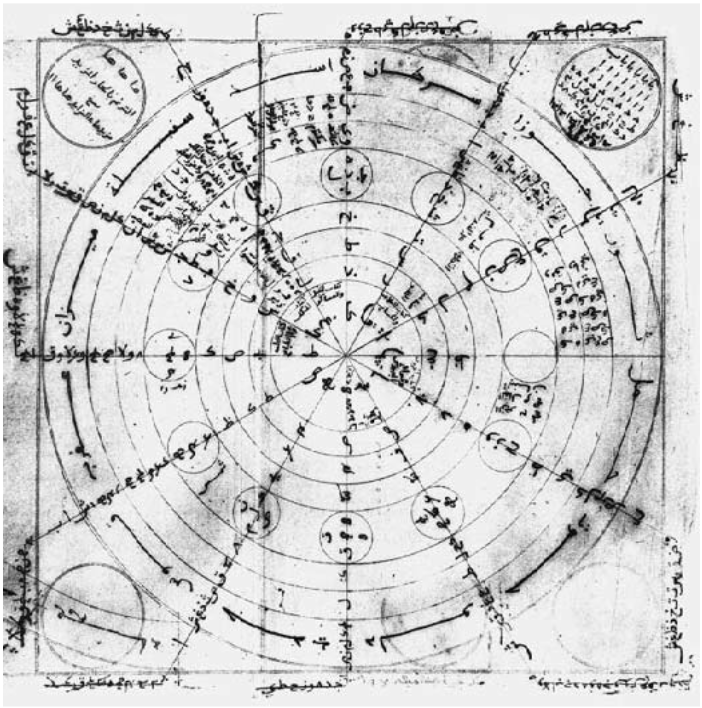
\includegraphics[width=0.49\textwidth]{ch1/images/zairja.png}
    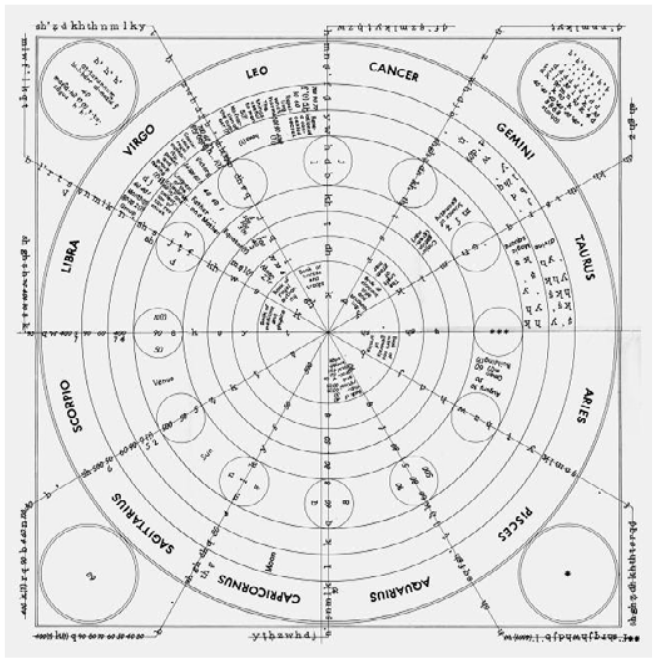
\includegraphics[width=0.49\textwidth]{ch1/images/zairjatl.png}
    
    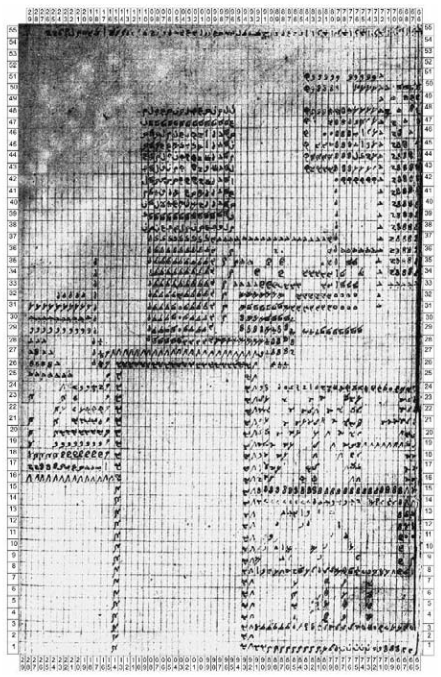
\includegraphics[width=0.6\textwidth,angle=90]{ch1/images/zairjaback.png}

    \caption{A zairja from a 15\textsuperscript{th} century Turkish manuscript of the \textit{Muqaddimah} \citep{link2010variantology}
        (top left), its transliteration from the English translation
    of \cite{rosenthal1958muqaddimah} (top right), and its lookup table (bottom).}
    \label{fig:zairja}
\end{figure}


{\color{red} Note to Kathy: the history of nlg sections are rough and I need to change them to reflect a new way of organizing the paper that I settled on so you can probably just skip ahead to section 1.4 on page 12.}

\section{A Brief History of NLG (antiquity-1950)}

The desire to build machines
that manipulate human languages is an old one. 
One early account of a language generation algorithm 
comes from 
14\textsuperscript{th} century historian 
`Abd ar-Rahm\={a}n ibn Khald\={u}n (1332 -- 1406), who
writes in the \textit{Muqaddimah} (1377) of a circular prognostication 
and divining tool  used by Sufi mystics called a \textit{z\={a}'irjah}.\footnote{Franz Rosenthal in his English translation of the  \textit{Muqaddimah} suggests the name is derived from 
the Persian words z\={a}'icha meaning ``horoscope'' or  ``astronomical table''
 and d\={a}'ira meaning ``circle.''}
 Its practice is
``a branch of the science of letter magic, practiced among the authorities on letter magic, is the technique of finding out answers from questions by means of connections existing between the letters of the expressions used in the question.'' 
Ibn Khald\={u}n points to an earlier treatise by the Sufi scholar 
Abu al-Abbas as-Sabti
(1129 -- 1204) of Marrakesh as a source of instructions for the device's use
\citep{rosenthal1958muqaddimah}, suggesting the practice is at least as
old at the 12\textsuperscript{th} century.

The \textit{z\={a}'irjah} itself consists of a series of concentric circles divided into 12 
sections by six chords. The various segments of the diagram are annotated with 
letters and numerals. Additionally, the \textit{z\={a}'irjah}  is accompanied by a lookup table mapping
letters to numbers. See \autoref{fig:zairja} for an example. According to painstaking reconstructions done by \citep{link2010variantology},
a ``key poem'' was used to pose a question to the \textit{z\={a}'irjah} and serve as a 
mnemonic device/mapping of letters to entries in the lookup table. 
A combination of rules and astronomical observations (the 12\textsuperscript{th} century equivalent of a random seed)
were then applied to the key poem to read off series of characters from
the \textit{z\={a}'irjah}. The operator
would then interpret those letters into an answer.  
``The fact that only consonants are written down in Semitic languages permits the meaningful interpretation of many random permutations of symbols,'' \citep{link2010variantology} suggesting that cherry-picking outputs and over-ascribing 
intelligence to a language generation algorithm are as old as the practice of
 NLG itself.

\begin{figure}
    \centering
    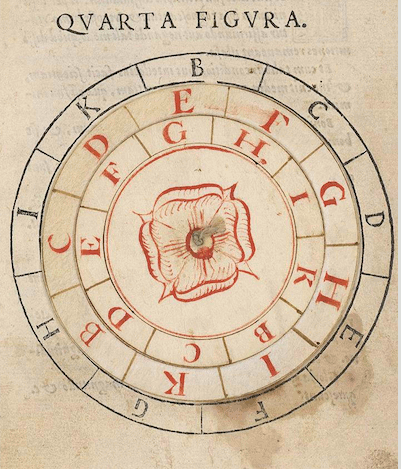
\includegraphics[width=0.48\textwidth]{ch1/images/llull.png}
    
\includegraphics[width=0.48\textwidth]{ch1/images/cipher.JPG}
    \caption{(Left) A \textit{volvelle} from  Llull's \textit{Ars Magnus} 
    and (right) Alberti's cipher disk.}
    \label{fig:llull}
\end{figure}

\begin{figure}
    \centering
    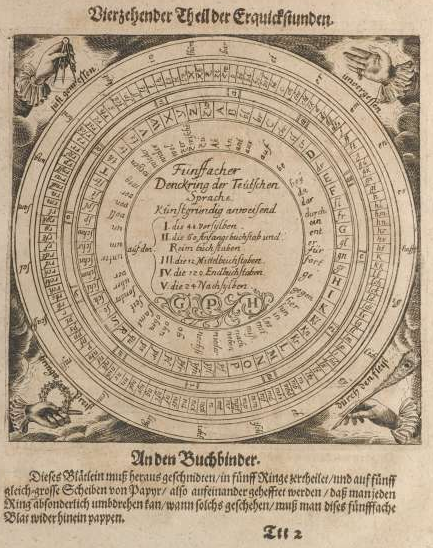
\includegraphics[width=0.98\textwidth]{ch1/images/baroqe.png}

    \caption{An illustration of the German word generator, \textit{F{\"u}nffacher Denckring der Teutschen Sprache}.}
    \label{fig:denckring}
\end{figure}



In a secondary account from a manuscript found at the library of Rabat, 
Morroco, it is written that a skeptical ibn Khald\={u}n asked of the device
how old it was: 
``[Is the] z\={a}'irjah [a] recent or [an] ancient science?'' 
and received the answer: ``The  Holy  Spirit  will  depart,  
its  secret  having
been brought forth / To Idr\={\i}s, and through it, 
he ascended the highest summit,'' drawing a connection to the sage
Idr\={\i}s who is one of the eldest
ancestors in the Quranic tradition \citep{rosenthal1958muqaddimah,link2010variantology}.



The teachings of Arabic mystics, including the practice of \textit{z\={a}'irjah}, as well 
as the Kabbalistic tradition embodied in the \textit{Sefer Yetzirah}
are known to have strongly influenced the 
Majorcan Christian mystic, Ramon Llull (1232-1315) \citep{kahn1980,sepllull,link2010variantology}.
%is known to have Arabic tradition  
%\textit{Z\={a}'irjah} are known to have influenced and similar practices from the Kabbalistic tradition 
%(the Sefer Yetzirah specifically) are known to have influenced the 
Llull, who is regarded as an early philosopher of combinatorics, logic, and 
computation \citep{sepllull,bonner2007art,knuth2013art}, developed 
a computational system based on moveable concetric circles made of paper
and connected by string. The workings of these \textit{volvelle}\footnote{The
    name \textit{volvelle} 
comes from the Latin, literally ``to turn''} are described in his master work,
\textit{Ars Magna} (1305). According to his system, concepts were assigned
letters which were manipulated to generate new knowledge and he claimed 
could be used to determine the truth of any proposition 
\citep{Crupi2019VolvellesOK}. Llull's work is also thought to have influenced 
the polyalphabetic substitution cipher developed by Leon Battista Alberti 
(1404 -- 1472) (see \autoref{fig:llull}), the same core cryptographic technology used 
in the Enigma machine  \citep{kahn1980}.


 \begin{figure}
    \center
    \noindent
    {%
        \setlength{\fboxsep}{0pt}%
        \setlength{\fboxrule}{1pt}%
        \fbox{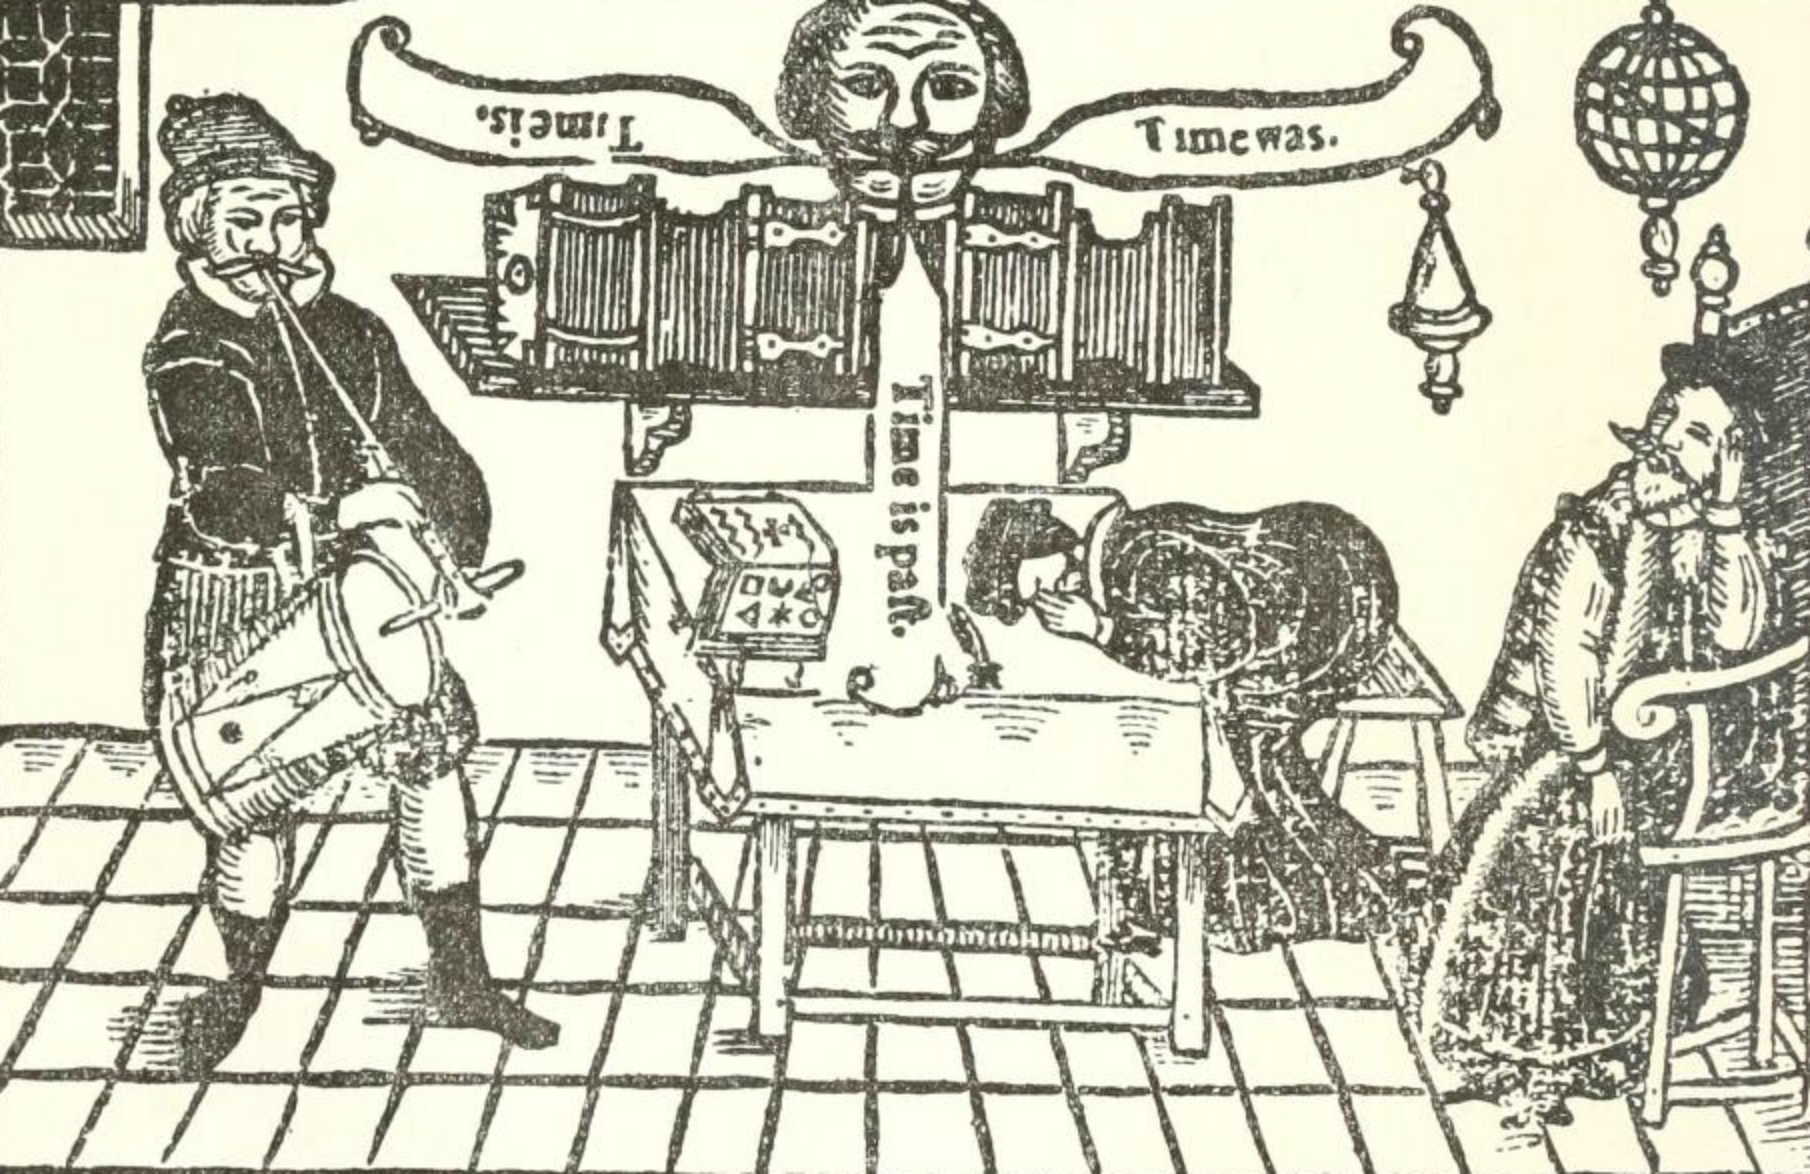
\includegraphics[width=0.7\textwidth]{brazen_head.png}}
}
\caption{A 1630 woodcut depicting Roger Bacon's talking bronze head, a mischievious talking autamata allegedly capable of answering any question \citep{hyman2016automaton}.}
\label{autamaton}
\end{figure}

\textit{Volvelle} were used throughout medieval Europe, arguably reaching
their zenith in the Baroque works of Georg Philipp Harsd{\"o}rffer (1607 -- 1658). His master work
\textit{volvelle},
\textit{F{\"u}nffacher Denckring der Teutschen Sprache} (1651), 
 consisted of five paper discs, and was claimed to faithfully model
 German word formation, and could aid in the production of poems and 
 other literary forms \citep{schafer2006literary}. See \autoref{fig:denckring}.



While computational devices before modern computing were limited in 
complexity by their construction
materials, chiefly paper, the dream of speaking automata was also
alive in myth.
See for example 
\autoref{autamaton}, in which a 17\textsuperscript{th} century woodcut print 
depicts a talking head capable of answering any question. This ``brazen head''
was allegedly built by the monk Roger Bacon, who in addition to being an
early philosopher of science and linguist, might also be considered 
the first natural
language processing (NLP) engineer if folklore is true \citep{sep-roger-bacon}.

%Depending on how loosely one defines an NLG algorithm, prayer, poem, and fortune generators have be found throughout many cultures in antiquity with
%prominent examples including volvelle \cite{} and lottery books \cite{}.
%Historical 
%evidence suggests these ideas were developed by Persian and Arabic scholars
%in the 9\textsuperscript{th}-??\textsuperscript{th} centuries \cite{},
%and eventually popularized in medieval Europe in the 13-1700s \cite{}. Volvelle
%are also notable for being used in early polyalphabetic substitution cyphers
% (the same core cryptographic technology used in the Enigma machine) \cite{}.


\section{A Brief History of NLG (1950-2010)}

Returning to the present day, computer aided 
production of human language closely follows the beginning of modern computing,
starting with work on machine translation (MT) systems developed 
in the 1950's and 60's \citep{ornstein1955mechanical,hutchins2003machine,national1966language}. Early work on producing extract summaries
of research articles also dates back to this period \citep{luhn1958automatic}.
There were also notable experiments in generating text purely from 
syntactic structures \citep{yngve1961random}.

However, NLG did not begin to coalesce as a distinct subfield until the 
1980s which saw
the first workshops devoted specifically to NLG  
and a convergence on the formalisms
and problems central to language generation \citep{reiter1997building,mcdonald2010natural}. 
NLG researchers of this period were focused on at least four
main research programs: (i) linguistically motivated grammars for generation,
(ii) frameworks for representating knowledge and concepts,
(iii) models of the human receiver of the generated text,
and (iv) models of discourse and control for planning the realization
of utterances \citep{mann1981text}. 


A variety of grammar and representation frameworks were proposed during this
period including Functional Grammar \citep{halliday2013halliday}, Transformational Grammar \citep{chomsky1965aspects}, Generalized Phrase Structure Grammar \citep{gazdar1985generalized}, \textit{et al.} and frameworks, including Knowledge
and Modalities Planner (KAMP) \citep{appelt1982planning}, Penman \citep{hovy1993natural}, MUMBLE \citep{McDonald1981MUMBLEAF}, TEXT \citep{mckeown1982text} and others \citep{mann1981text}.
While there appears to be a great diversity of approaches, most approaches
seem to converge on a fairly similar pipeline of modules when it came 
it implementation \citep{reiter1994has}. 

In particular, most NLG systems from this
period could be understood as a pipeline of modules for text planning,
sentence planning, and linguistic realization \citep{reiter1997building}.
In the text planning stage, the concepts to be conveyed are selected,
possibly discarding less essential information, and arranged into a discourse
plan or ordering. In the sentence planning stage,
the concepts from the previous stage are grouped into individual sentences,
and lexicalization of concepts and referring expression generation is performed.
Finally, in linguistic realization, the intermediate representation from 
the sentence planning stage is converted into a natural language utterance,
often by linearizing and inflecting some syntactic/morphological representation.

Since these systems primarily started from a non-linguistic representations 
of concepts, they are often referred to as 
\textbf{concept-to-text} generation or, as more commonly known today, 
\textbf{data-to-text} generation
\citep{gatt2018survey}. These systems were applied to a variety of data-to-text
problems including weather forecast generation \citep{goldberg1994using},
statistical report  generation (i.e. generating a report from numerical
or stastical data in a spreadsheet) \citep{iordanskaja-etal-1992-generation},
or as a writing aid to improve the productivity of human authors ().
Data-to-text generation came to prominence alongside expert systems \citep{todd1992introduction},
including as a means to explain them \citep{swartout1983xplain},
and often suffers from similar drawbacks. NLG systems often required extensive 
domain knowledge and manual rule or grammar engineering.

In the late 1990s and 2000s, as larger text corpora became available and statistical 
and/or machine learning techniques spread through the community, 
\textbf{text-to-text} generation (i.e. methods
of directly mapping unstructured text inputs to text outputs) increased in
popularity. Text-to-text generation is less defined by a specific 
generation task, method or unifying
theory, but on the use of large collections of example input/output text pairs.
For example, machine 
translation (MT), text simplification, and text summarization 
are all considered text-to-text generation when the approach uses
aligned sentence in input and output languages, pairs of complex and simple
sentences with similar meaning, and document/summary pairs respectively.


Some graph summarization  stuff.

Work on supervised learning for summarization begins to emerge from this
time \citep{kupiec1995trainable,osborne2002using,hirao2002extracting}. In these data-driven approaches, summarization
is framed as a sentence classification task, i.e. which sentences from the
input document should be included in a summary. While significantly constrained
in their expressive quality (i.e. only sentences found in the input can be
used to construct the output) especially compared to earlier data-to-text methods, designing features and focusing on the learning algorithm for performing
the generation task proved to be much more scalable. 
The Document Understanding Conferences start in this time, bringing together 
NLP researchers, particularly around multi-document summarization \cite{duc}.

The ability to generate more interesting or novel text also gradually increased
with time. In the unsupervised case sentence fusion \cite{fusion};
in the supervised case, learning syntax guided compression and extraction
appeared \cite{} although generation was still dificult and abstractive summarization was rare \cite{maybemckeownnenkova}.



\section{A brief history of NLG (2010-present)}

While neural networks had been used previously as part of phrased-based 
statistcal MT (SMT) systems \cite{}, there was an increased interest in
the early-mid 2010's around using recurrent neural network (RNN) language 
models \citep{miklov}
as a rescoring method for an SMT decoder \citep{auli2013joint,cho2014learning}.
While previous approaches 
used feed-forward networks, RNNs could exploit (in theory) unbounded source
and target prefix information that was difficult to caputre in n-gram or 
feed-forward models. \citet{cho2014learning} is particularly noteable because
they propose separate encoder/decoder RNNs, and while intended for rescoring
and not generation directly, this general architecture 
constitutes ``sequence-to-sequence'' backbone of most neural MT (NMT) and 
neural NLG models.

Shortly thereafter, \citet{sutskever2014sequence} proposed the now ubiquitous 
sequence-to-sequence model to perform translation directly. \citet{bahdanau2015neural} (2014 on arxiv) also propsed a sequence-to-sequence model with 
an attention mechanism, which both made optimization easier, (error feedback,
 i.e. gradients, could now be routed directly from any decoder word prediction 
 step to
 any arbitrarily  distant timesteps in the encoder)
 and allowed for visualization of NMT decoder's alignment with the encoder
 (see \autoref{fig:nmtattn}).
NMT models, while conceptually simpler than phrase-based SMT, were starting
to achieve state-of-the-art results \cite{} and wide-spread industry adoption
\cite{wu2016google}.

It did not take long for researchers to adapt the sequence-to-seqeunce model
to other language generation problems, e.g. generating captions from images \cite{},
sports summaries for box scores \cite{}, or, echoing the dreams of 80s NLG, 
from semantic representations \cite{}. In summarization, sequence-to-sequence
models were quickly adapted to generate headlines and eventually full summaries\cite{}, and copy-mechanisms were developed to blur the extractive/abstractive
summarization distinction \citep{}. Given parallel object/text pairs,
it now became increasingly easy to develop a plausible conditional NLG system,
while far from perfect \cite{}, it is hard to under-estimate effects
of the deep learning paradigm on language generation.

In \citeyear{vaswani2017attention}, \citeauthor{vaswani2017attention}
proposed a recurrence-free neural sequence model, built around so-called 
\textit{transformer} layers,
which rely on mulitiple parallel self and context attention mechanisms.
This model was designed with optimization speed in mind, and was subsequently
used in large scale language modeling pretraining on web-scale text, 
spawning the BERT-family
of models \citep{}. BERT has since been used as a non-autoregressive means
of generating text \citep{}. 

The transformer layer was also used in the (generative pre-training) GPT
family of models \citep{}, which also trained on web data, but with an
auto-regressive language modeling objective. The second generation of 
these models, GPT-2, reveived notoriety both amongst NLP researchers but 
also the wider public, as it's release was initially delayed given ``ethical
concerns'' about releasing such a powerful language generation model \citep{}.
Regardless of the merits of these claims, the model was eventually released
and does exhibit impressive prefix capabilities, generating longer spans
of fluent text than previously thought possible. 

Like BERT, GPT-2 could used in a fine-tuning setting, and used in a 
variety of conditional generation settings \citep{}. BART \citep{bart} and
T5 \cite{t5} followed with sequence-to-sequence variants of the 
large transformer-based model pretrained on denoising autoencoder and 
other pretraining objectives, where both models are designed to be fine-tuned
on sequence-to-sequence language generation tasks. 


\section{Problems in Text-to-Text Generation}

As envinced by this brisk journey through the history of \languagegeneration,
\machinelearning~has emerged as the \latin{de facto} methodology for 
solving both \texttotext~and~\datatotext~problems. \Deeplearning~models in 
particular have shown themselves to be both versatile and empirically 
successful solutions. However, the inner workings of such models are often 
opaque and difficult to 
control or understand in practice. In this thesis, we offer modeling 
methodologies to establish control or understanding in a variety of  
\machinelearning-based models of summarization. At a high level, the 
first two chapters focus on \contentselection.
The last chapter focuses on \surfacerealization, that is, generating text
from an idealized representation of the content selection stage. 
%in the idealized case of problems, effectively focusing
%on the actual language generation component, i.e. how to say it. (note to self, cite Kathy's work here).

In this section, we will briefly introduce the tasks and problems that will 
ground the experiments and analyses of this work. More formal definitions
can be found in the individual chapters. 
%It is for this reason that we focus on extractive summarization in this work.
%\Automaticsummarization~as it is studied in the 
%\naturallanguageprocessing~literature typically dichotomizes summarization
%approaches into either \extractive~versus \abstractive~methods \cite{something}. 
%In the former case, a summary is constructed by essentially copying and 
%pasting the input utterances to obtain a summary; in the latter case, the 
%summary content is generated from scratch, synthesizing the input content in
%some manner to produce the summary. In practice, systems are often composed of
%a mixture of extractive and abstractive techniques, e.g., using sentence 
%compression on top of extraction. We study the extractive task since it allows
%us to focus on the salience estimation task directly, while not having to
%implement an abstractive generation component (which is typically more
%computation and memory intensive than, and more difficult to evaluate). 
%
%
%
In most summarization problems, we are generally interested inf 
a text's \textit{\salience}, that is to say, the general importance or relevance of 
a given text unit with respect to its context. \Salience~is usually the primary dimension of the input data that we wish to 
measure or predict for summarization problems. 
In \autoref{dlsal}, we study \salienceestimation~in 
the \emph{sentence extractive, single document summarization task}, 
where the goal is to classify which sentences in an input document should be 
included in an extract summary. 
In this case, the input document is the context, and the units of text for 
which we are estimating salience are the document
sentences. An extractive summary is a subset of sentences that have maximum
salience while sastifing a length budget constraint, typically in the summary
word or byte length. While the constrained subset selection problem is 
interesting and has been studied previously \cite{maybemmr,mcdonald,others},
we focus on modeling the salience estimation task specifically. 

%?Since salience is not usually explicitly available in most summarization 
%?datasets, we approximate it by first constructing an extract summary from input
%?document the greedily maximizes a measure of ngram overlap with a human
%?reference abstractive summary subject to the length constraints. We then
%?consider as salient those sentences which were select for the extract 
%?summary.

We study a variety of popular and novel \deeplearning~architectures for 
implementing the salience prediction task. Our key contribution here is not
a modeling architecture, but our systematic study of the combination of 
sentence and context (i.e. document) level encoders as well as the 
manipulation of the input documents to ablate which surface features are 
available to a given model. Through these input data ablations, we can gain
a better understanding of how the salience prediction mechanism is working.


In \autoref{mlsal}, we study a more difficult summarization task, 
\emph{query focused, streaming, sentence extractive summarization}. In this
task, we add a search query and time as additional elements to the 
summarization problem. As input we are given a time-ordered stream of news 
articles and a query, typically an notable real-world event, 
e.g., \texttt{``Hurricane Sandy''}. Our objective is to extract sentences that
are relevant to the query event while minimally redundant to previously 
extracted
sentences. Unlike the previous problem, the salience of given sentence 
is not constant but monotonically decreases as time goes on. In addition
to modeling the salience, we must now also model the redundancy between
sentences. 

The main contributions of this work are to show that with careful feature 
design, we can capture salience beyond using the position-based heuristics
that we found the neural models to use. In particular, we show that content
based, time, location, and redundancy features can be used to predict salience
in this more challenging scenario.

We encorporate these features into two possible approaches for streaming
summarization.
The first method works in time ordered batches, processing all sentences that 
occur in \autoref{times}-hour windows of the news the stream. The actual summarization method happens in two stages. In the first stage salience of the individual
sentences is estimated. Then, those salience predictions are used to bias
an exemplar base clustering algorithm, such that the cluster centers are both
representative of cluster members but also highly salient. 


The second method works by making sequential prediction on sentences from 
the input news stream immediately, without batching or waiting to collect 
a reservoir of a certain size. This model employs a learning-to-search style
of algorithm \cite{searnorlosl} to avoid exposure bias inherent to these
extended sequence prediction tasks.


In \autoref{gen}, we move to problems of \surfacerealization~after the content
selection process has been performed. 
Here we focus on the related goals of
\term{faithful}~and~\term{controllable}~generation. A faithful language 
generation model generates utterances that are semantically correct
with respect to the information extracted in the 
content selection stage.
%a reframing of the evaluation of \naturallanguagegeneration~from fluency and
%to semantic correctness 
Controllable generation models represent a subset of 
faithful generation models. Controllable generation models follow
an explicit plan that guides the surface realization order of the generated utterance.
Faithful but uncontrollable models will generate semantically correct 
utterances but the decoder language model implicitly controlls the surface
realization order by generating the next utterance word.

Evaluating the faithfulness of a language generation model for open-world
summary generation tasks is non-trivial. In order to simplify things,
we study faithful and controllable generation in the context of 
\emph{\taskorienteddialoggeneration}, 
 where given an explicit representation
of a dialog agent's belief state and goals, we must generate an appropiate
natural language utterance. Because the input is an explicit, formalized 
representation of the meaning of the intended utterance, manual and 
even automatic checking of the faithfulness of an
utterance/meaning representation pair becomes much simpler. Since the concerns
of faithful and controllable generation are still relevant to generating
summaries, we consider the explicit meaning representations as 
an idealized version of summarization system's content selection stage.


%In \taskorienteddialoggeneration, the dialog agent
%has a communicative goal that it is trying to achieve. Crucially,
%the input to the agent is an explicit representation of the meaning 
%of intended utterance.
%
%
%In \autoref{gen}, we move to the \datatotext~problem of 
%\emph{\taskorienteddialoggeneration}, where given an explicit representation
%of a dialog agent's belief state and goals, we must generate an appropiate
%natural language utterance. In \taskorienteddialoggeneration, the dialog agent
%usually has a goal that they need to achieve. For example, a dialog agent may
%want to book a reserveration at a restaurant but inorder to do that, it 
%needs to ask a user for a range of possible times that are acceptable to
%place the reservation. In this case, input to the dialog generation 
%component would be a representation describing a \texttt{request information} dialog act, with the desired missing information explicitly represented,\texttt{reservation time range}.
%
%When deep learning models are used to generate text in scenarios like these,
%they are usually effective at generating fluent and natural text \cite{}.
%However, without careful treatment, the frequently generate utterances
%that do not accurate reflect the input meaning representation. In the
%case above for example, they might accidentally request the  location 
%instead of the time. 


For our contribution to faithful generation, we propose a novel 
data augmentation method that uses an unfaithful NLG model and an NLU model 
to generate novel and semantically diverse utterance/meaning representation 
pairs that can be used as additional training data. Sequence-to-sequence
models trained on the union of original training data and the synthetically
generated training examples exhibit increased faithfulness.

% to remove spurious correlations from the 
%training data and obtain a 
%neural \naturallanguagegeneration~model with reduced semantic errors.

While this data augmentaiton method helps reduce semantic errors, it leaves the surface
realization of utterances up to the decoder language model. In \autoref{gen}
we also investigate an encoder input transformation, applicable to arbitrary \sequencetosequence~models, that reliably results in a controllable generation 
model. 


%
%it occurs in)
%
%We start in the single document extractive summarization case, 
%where the task is 
%to predict a subset of an article's sentence to include in a summary.
%We explore several popular neural architectures for performing this 
%task and systemaically evaluate them under different noisy input ablations.
%These ablations allow us to isolate different features of the input.
%
%
%In the second chapter, we explore two classical machine learning models
%applied to the harder problem of query focused extractive stream summarization. 
%In this setting we propose two models, one that 

\section{Contributions}

We now briefly summarize the contributions of this thesis described
in the previous sections.

%This thesis  makes the following contributions to NLG.
%In the areas of text-to-text generation,

\begin{enumerate}
        \item We propose a systematic evaluation of deep learning models
            for extractive single document summarizations (\autoref{}). 
            Our evaluation on several popular neural architectures shows 
            that:
            \begin{itemize}
                \item Position features, even when not explicitly represented
                    in the model architecture are a dominant feature
                    exploited by the model.
                \item Content features exist across a variet of word classes
                    but are not as strong of a signal as position.
                \item Word embedding averaging is about as effective as 
                    recurrent or convolutional sentence encoders 
            \end{itemize}
        \item Additionally, in the task of query focused streaming news 
            summarization, we propose two models for providing 
            extractive update summaries. (\autoref{})
            \begin{itemize}

                \item The first method processes the stream in  batches. 
                    It uses a regression model
                    to estimate the salience of individual 
                    sentences, and a biased clustering algorithm to select
                    the most representative and salient outputs.
                \item The second method processes the stream in a fully
                    online manner. A linear model makes extraction
                    decisions, and we experiment with a learning-to-search
                    algorithm for training. 
            \end{itemize}
    \end{enumerate}

    In the area of data-to-text generation, we make the following 
    contributions to faithful and controllable generation of 
    text from a meaning representation. 
    \begin{enumerate}
        \item We propose a noise injection and self-training method
            for obtaining a faithful NLG model.
        \item We propose an encoder input linearization called alignment
            training which  yields an NLG model with surface level
            realisation ordering control.
    \end{enumerate}


Finally, in chapter \autoref{conc} we conclude with a discussion of the 
limitations and future 
directions this work might take. In particular, we focus on how 
faithful generation might be applied to summarization or \machinetranslation
where an explicit representation of the content meaning is not available. 







%%%%%%%%%%%%%%%%
%% Chapter 2
%%%%%%%%%%%%%%%%%


\chapter{Deep Learning Models of Salience Estimation }
\label{dlsal}
\section{Introduction}

\Salienceestimation, that is, the prediction of 
the importance or relevance of a unit of text, is a critical step
for any \textsummarization~algorithm \citep{nenkova2011automatic}. Since the size of 
the desired output summary is constrained to be much smaller than the original
document or documents being summarized, it is necessary to prioritize 
some information over others when deciding the content of  the summary. Estimating the \salience~of various units of text (i.e., words, phrases, sentences, etc.) enables summarization algorithms to perform this 
prioritization.

 There is no universally agreed upon 
definition of salience, so its estimation starts on rather shakey 
epistemological ground. What is most \salient~will vary significantly from 
reader to reader,
and depend largely on their particular information need and/or prior knowledge
\citep{jones1999automatic}.
In this chapter, we focus on a supervised learning scenario, where 
the training corpus consists of a single document paired with a human reference abstract summary prepared
by a domain expert. In this setting,  we can rely on a data-driven definition
of \salience;
information that the domain expert has put in the summary is most salient.
By matching units of text in the input document to corresponding text units
in the summary, we label the document text units with a binary judgement of
\salience~(see \autoref{sec:labelgen} for details). 

If we set the basic unit of text to be a single sentence and we obtain binary
\salience~judgements in the manner described above, we can model
sentence extractive single document summarization as a sequence labeling 
task \citep{conroy2001}. In this formulation, a document is a sequence of 
sentences, and the task objective is to predict the salience judgment
for each sentence. In the simplest of settings, the actual \extract~summary
can be formed by concatenating the sentences labeled as \salient.
%with the goal of labeling each unit with one of two labels: \emph{\extract}, this
%unit is \salient~and should be added to the extract summary, or \ignore, this 
%text unit is of low or zero \salience~and 
%text should be discarded from the summary. 


We refer to the probability of a sentence being labeled as \salient~as the 
\salience~estimate.  Historically, most \machinelearning~based methods for salience estimation
have use \featurebased~representations of text units to make 
\salience~estimates. Typically, these features make use of word level 
frequency data \cite{a,b,c}, information theoretic notions
of suprisal or topicallity \cite{x,y}, as well as position based features
(e.g., is the unit of text in the beginning, middle, or end of the document?)
\cite{position},
which are often correlated with human judgements of salience.


The field of summarization has not been unaffected by the recent popularization of \deeplearning~based models in \naturallanguageprocessing.
\Deeplearning~models
have demonstrated empirical successes, achieving state-of-the-art 
performance in both \extractive~\citep{somepeople} and \abstractive~summarization 
settings \citep{someothers}. \Deeplearning~models also naturally allow for learning
hierarchical representations of word, sentence, and document
level contexts when performing end-to-end training on the summarization 
task.
However, exactly what kind of information is captured in these representations
and how that information effects downstream salience estimation has not 
been experimentally verified. 


In this chapter, we systematically compare several supervised 
\deeplearning~models of sentence extractive single document summarization.
As in prior work, we model a document hierarchically: a document is 
a sequence of sentences and a sentence is a sequence of words. 
Each summarization model consists of three layers or modules: 
\begin{enumerate}
    \item The word
embedding layer, which maps sequences of words to sequences of fixed 
dimensional embeddings. 
\item The \sentenceencoder~layer, which
maps sequences of word embeddings to a sentence embedding. 
\item The 
\sentenceextractor~layer, which maps sequences of sentence embeddings to
a sequence of \salience~judgements.
\end{enumerate}

We systematically compare three different architectures for the \sentenceencoder~and four different \sentenceextractor~architectures. Additionally, 
we also measure the effect of using fixed pretrained embeddings versus 
fine-tuning embeddings while training the rest the of model. 
Various configurations of \encoder~and \extractor~modules correspond to
both prior works as well as novel summarization models. While prior works 
have primarily used \autoregressive~\sentenceextractor~architectures, we propose two
\nonautoregressive~\sentenceextractor s.
We evaluate these
models across a range of domains including large and small news domains,
as well as personal stories, meetings, and medical research articles. 



Additionally, we systematically ablate the inputs to models during 
training to better understand what surface level features are being 
used to make predictions. Words are tagged with a \partofspeech~tagger
and different word classes are replaced with special \emph{unknown} tokens.
We can then compare performance of the summarization model with and without
access to specific classes of word features (e.g., nouns or verbs). To 
ablate the implicit effects of sentence position, we compare models
trained on the original document to the same model trained on documents
with shuffled sentence order. By removing content and position features,
we can see their relative impact in the decrease in \rouge~scores on the 
test set. Moreover, these ablations give us a more intuitive understanding
of how models will behave in novel environments. For example, if we know
position is an important feature for a model, using it on data that is
not position biased will likely result in poor performance.


Our main results  reveal:
\begin{enumerate}
 \item Sentence position bias dominates the learning signal for news summarization, though
not for other domains. Summary quality
for news is only slightly degraded when content words are omitted from sentence embeddings.
\item Word embedding averaging is as good or better than either RNNs or CNNs for sentence
embedding across all domains.
\item  Pre-trained word embeddings are as good, or
better than, learned embeddings in five of six
datasets.
\item Non auto-regressive sentence extraction performs as good or better than auto-regressive
extraction in all domains.
\end{enumerate}

Taken together, these and other results in the paper suggest that we are over-estimating the ability of deep learning models to learn robust and
meaningful content features for summarization. In
one sense, this might lessen the burden of applying neural network models of content to other domains; one really just needs in-domain word embeddings. However, if we want to learn something
other than where the start of the article is, we will
need to design other means of sentence representation, and possibly external knowledge representations, better suited to the summarization task.

%In the next sections, we formally define the extractive summarization 
%problems, and our proposed models for solving this problem. We then
%d

%\pagebreak


%?Before formally defining our summarization problem, and models, 
%?
%?
%?Ablations include position (i.e., sentence order is
%?`shuffled) and word classes (i.
%?
%?Words are 
%?represented with embeddings. A \sentenceencoder~a neural network that
%?maps a sequence of sentence 
%?
%?
%?
%?
%?
%?
%?However, the exact nature of the useful signals encoded in these representations has not been verified beyond high level motivations for architecture
%?design choices.
%?
%?
%?%In \featurebased~\machinelearning~models of \salienceestimation,
%?%When modeling extractive summarization as a sequence labeling problem
%?Historically, \salienceestimation~has been explicitly modeled 
%?as part of the larger summarization task (c.f. \cite{somebody}). Under
%?some extractive approaches, \salienceestimation~amounts to the entirety of the summarization
%?process \cite{something}.
%?
%?In practice most supervised \machinelearning~approaches estimate
%?
%?
%?In practice most supervised \featurebased~\machinelearning~approaches resort 
%?to approximating \salience~with some proxy feature. Common proxies typically work from
%?term frequency information \cite{a,b,c} or information theoretical notions
%?of suprisal or topicallity \cite{x,y}, essentially words that occur frequently
%?in the input document but infrequently in some background corpus (which
%?is itself a proxy for a reader's prior knowledge).
%?
%?
%?
%?%Naturally, there is no universal definition of \salience, as 
%?%what is most important will vary significantly from reader to reader,
%?%depending largely on the reader's information need and/or prior knowledge
%?%of the information being summarized. To make 
%?%
%?
%?%Typically, i
%?
%?
%?While \salienceestimation~has historically been modeled explicitly
%?(e.g., \cite{somebody}), with the move to end-to-end 
%?\deeplearning~approaches, it is often
%?assumed to be happening implicitly in a model's hidden layers.
%?
%?
%?Both extractive and abstractive \deeplearning~summarization models have 
%?demonstrated empiracle success with state-of-the-art performance on automatic 
%?metrics like \rouge \cite{rouge}. 
%?The success of the \deeplearning~approach partially stems from the ability to 
%?flexibly and hierarchically learn word, sentence, and document representations.
%?However, the exact nature of the useful signals encoded in these 
%?representations has not been verified beyond high level 
%?motivations for architecture design choices.
%?
%?
%?
%?
%?
%?%representation learning, it is unclear what signals they are extracting
%?%from the data to make predictions.
%?
%?
%?%However, it is not well understood how \deeplearning~models perform salience estimation with only word, sentence, or document embedding
%?%based features as input. 
%?
%?
%?
%?Increasingly, deep neural 
%?network models are being used to perform sentence extractive summarization 
%?tasks. While these models are very flexible and allow for easy hierarchical 
%?representation learning, it is unclear what signals they are extracting
%?from the data to make predictions.
%?In this section, we describe our completed experiments teasing out the 
%?importance
%?of different neural network designs for sentence level salience estimation
%?\cite{kedzie2018deep}. 
%?In particular, we experiment with several methods for encoding a sequence
%?of word embeddings into a sentence embedding, and then in turn, mapping
%?a sequence of sentence embeddings to sentence salience predictions. We 
%?introduce several simplifications to existing models in the literature, and
%?show their effectiveness on an SDS task across news, personal narratives,
%?workplace meetings, and medical journal article genres.
%?
%?We also perform several diagnostic experiments 
%?and find impediments to learning robust models of 
%?sentence salience. In particular, the sentence position implicitly 
%?encoded in the models dominates the learning signal. While sentence position
%?is certainly an important feature in news, not all domains or tasks 
%?will share this feature;
%? we would also like to be able to design
%?models that make their salience decisions primarily on lexical or
%?topical content.
%?
%?We believe that the sentence embedding representation is too coarse to
%?make significant use of lexical information in the presence of less noisy
%?position features, even when position is only implicitly represented by 
%?the model.
%?To that end, we propose a new deep learning based SDS model that directly 
%?estimates individual word level salience scores, and a simple sentence 
%?selection and margin loss framework for learning. In this model,
%?we augment the word embeddings (which only capture shallow lexical semantics)
%?with embeddings representing other word features. Our initial experiments
%?suggest that document frequency, and information theoretic accounts of 
%?surprisal (e.g. topic signatures) are also useful for the summarization task. 
%?We expect to show less dependence on the position features using
%?the same ablation diagnostics we applied to our sentence level salience 
%?models. 
%?While previous work has estimated word importance using these features
%?in a linear model 
%?\cite{hong2014improving}, they were only able to take limited advantage of 
%?context features, i.e. taking a weighted average of word features to
%?the left and right. By contrast,
%? in our proposed model we can combine rich
%?document specific contextual features, e.g. \textsc{Elmo} embeddings 
%?\cite{peters2018deep}, in conjunction with these word features.
%?
%?Additionally, we plan to adapt this word level salience model to a news MDS task;
%?if it is less dependent on sentence position, it should be more amenable 
%?to MDS where lexical centrality to the document cluster is possibly
%?the dominant learning signal.  
%?%We concluded this section with proposed domain adaptation experiments for
%?%modifying the word importance model to work on a news MDS task. 
%?The MDS version of the model will use an importance score aggregation step
%?where word level scores accrue additional importance across documents 
%?using an attention mechanism.
%?
%?
%?In the next subsections we first briefly cover related work on sentence
%?and word level salience estimation before covering the 
%?completed sentence level
%?and proposed word level salience estimation experiments.
%?%are the
%?%This
%?%work describes impedements to learning and word and sentence representations
%?%in deep learning models of extractive summarization, and led to 
%?%a recent publication \cite{kedzie2018deep}. Based on these limitations,
%?%we propose extensions to the word level representations and explicitly model
%?%word level salience scores as a means to performing sentence extractive
%?%summarization. While the finished and proposed work focuses on single document
%?%summarization, we also propose an extension of the word level salience
%?%estimation model that we hope will generalize to the multi-document
%?%summarization context.
%?
%?
%?
%?
%?
%?%\hal{i feel like you can restructure the intro to focus on you stuff, rather than focusing on how it relates to other people's stuff. just lead with context selection is important for generation, summarization, etc., and is a key compontent both in extractive *and* abstractive techniques. then go to the third paragraph about what you do. you can then relate back to deep learning predictions in the related work section.}
%?
%?%While there has a been a recent flurry of work on abstractive summarization
%?%\cite{paulus,see,chenglapata,nallapati},
%?%these papers treat this problem as a pure sequence to sequence 
%?%transduction task. Admittedly, this view allows us to apply very powerful, 
%?%general-purpose deep learning archictures to generate summaries.
%?%At the same time, it obscures a principal subtask in summarization, the 
%?%process of selecting the most salient units of meaning in the source material,
%?%i.e. the key ingredients in the final summary, a process which we 
%?%broadly refer to as content selection \cite{possiblyMcKeownAndNenkova}.
%?
%?%As is also the case in other NLP tasks, it is not immediately obvious how a
%?%deep learning model is making its predictions, or what correlations 
%?%are being exploited. There is a concerning and growing list of papers that 
%?%find models functioning as mere nearest neighbors search 
%?%\cite{liang,danqichen}, exploiting annotator artifacts 
%?%\cite{recentNaaclPapersOnSNLI}, or open to adversarial exploitation \cite{findExampleYouNoMemoryDumbDumb}. 
%?%These lines of research are critical for finding model shortcomings, and over
%?%time, guiding improvements in technique. Unfortunately,
%?%to the best of our knowledge, there has been
%?%no such undertaking for the summarization task. 
%?
%?
%?%\kathy{content selection is very different for generation than for summarization.
%?%I think you need to initially say that content selection for generation is sentence
%?%selection. Note that you could be criticized even here as some people may say that
%?%summarization should be phrase selection (although it rarely is)}
%?%\kathy{I have also reworded definition of content selection for NLG.}
%?Content selection is a central component in many natural language generation
%?%problems, 
%?tasks,
%?where, given a generation goal, the system must determine which information
%?%i.e. given some context, determine which information
%?should be expressed in the output text \cite{gatt2018survey}.
%?In summarization, content selection is usually accomplished through sentence (and,
%?occasionally, phrase) extraction.
%?Despite being a key component of both
%?extractive and abstractive summarization systems, it is is not well
%?understood how deep learning models perform content selection with only word and 
%?sentence
%?embedding based features as input.
%?%\hal{i'm not sure what this sentence means, especially the part after ``using'', CK: addressed it, does it work now?}.
%?%\hal{well understood as a task or in specific models?} 
%?Non-neural network approaches often use frequency and information theoretic measures as proxies
%?for content salience \cite{hong2014improving}, but these are not explicitly %\hal{directly? explicitly?} 
%?used in most neural network summarization systems.
%?%\hal{maybe instead of recent work say nn systems?}.
%?% changed wording
%?
%?%\hal{there are lots of widows/orphans throughout that need to be cleaned up.}
%?
%?In this paper, we seek to better understand how deep learning models of 
%?%summarization are performing content selection across a variety of domains.
%?summarization perform content selection across multiple domains (\S~\ref{sec:datasets}): news, personal stories,
%?meetings, and medical articles (for which we collect a new corpus).\footnote{Data preprocessing and implementation code can be found here: \url{https://github.com/kedz/nnsum/tree/emnlp18-release}}
%?%no new paragraph needed here
%?We analyze
%?several recent sentence extractive neural network architectures, 
%?specifically considering the design choices for sentence encoders (\S~\ref{sec:senc})
%?and sentence extractors (\S~\ref{sec:sext}). We compare Recurrent Neural Network (RNN) and Convolutional Neural
%?Network (CNN) based sentence representations to the 
%?simpler approach of word embedding averaging to understand the gains 
%?derived from more sophisticated architectures.
%?We also question the necessity of auto-regressive sentence extraction 
%?(i.e. using previous predictions to inform future predictions), 
%?which previous approaches have used (\S~\ref{sec:related}),
%?and propose two alternative models that extract sentences independently.
%?%
%?%We compare these architectures against
%?%a simpler approach based on averaging of word embeddings in order to understand
%?%the gains derived from more sophisticated architectures.
%?%
%?%\kathy{I would find it better to introduce approach here. I've added an
%?%extra sentence above. Because your experiments reveal the tidbits below by 
%?%contrasting past approaches with your simple approach which uses embedding
%?%averages}
%?%
%?%
%?%\kathy{You use some strong words, one of which is ``worrying''. I think it
%?%may be better toned down. After all, reviewers may be Lapata or Nallapati}
%?%\kathy{Also, I think it should be pumchier with all learned things itemized.
%?%For example:
%?%~
%?%KM2: Minor changes below
%?\\[-0.5em]
%?
%?\noindent
%?Our main results (\S~\ref{sec:exps}) reveal:
%?\begin{enumerate} %[noitemsep]
%?\item Sentence position bias dominates the learning signal for news summarization, though not for
%?    other domains.\footnote{This is a known bias 
%?    in news summarization \cite{nenkova2005automatic}.}
%?        %\hal{be consistent on domain/genre. also maybe you should say above what domains you consider?}. 
%?Summary quality for news is only slightly degraded when content words
%?are omitted from sentence embeddings. %\hal{this sounds like you remove content words and the summary is still as good. clearly not what's meant. i hope :P.}
%?\item Word embedding averaging is as good or better than either RNNs or CNNs for sentence embedding across all domains.
%?\item Pre-trained word embeddings are as good, or better than, learned embeddings in five of six datasets.%\hal{you were specific in the other ones, be specific here too if possible}
%?\item Non auto-regressive sentence extraction performs as good or better 
%?     than auto-regressive extraction in all
%?    domains.
%? %   Representation of previously selected summary content does not improve overall summary content. \hal{i think this one might be hard to parse for non-experts. maybe ``explicitly reprsenting prev...''}
%?\end{enumerate} 
%?
%?\noindent
%?Taken together, these and other results in the paper suggest that we are 
%?over-estimating the ability of deep learning models to learn robust and 
%?meaningful content features for summarization.  
%?In one sense, this might lessen the burden of applying neural network models
%?of  content to other domains; one really just needs in-domain word embeddings.
%?However, if we want to learn something other than where the start of 
%?the article is, we will need to design other means of sentence representation,
%?and possibly external knowledge representations, better suited to the summarization task.
%?

%%% Local Variables:
%%% mode: latex
%%% TeX-master: "dlextsum.emnlp18"
%%% End:

%
\section{Related Work}

The introduction of the CNN-DailyMail corpus by \citet{nips15_hermann} 
allowed for the application of large-scale training of deep learning models 
for summarization.
\citet{cheng2016neural} developed a sentence extractive model that uses a 
word level CNN to encode sentences and a sentence level sequence-to-sequence 
model to predict which sentences to include in the summary. Subsequently, 
\citet{nallapati2017summarunner} proposed a different model using word-level 
bidirectional RNNs along with a sentence level 
bidirectional RNN for predicting which sentences should be extracted. 
Their sentence extractor creates representations of the whole document and 
computes separate scores for salience, novelty, and location.
These works represent the state-of-the-art for deep learning-based extractive
summarization and we analyze them further in this paper.

Other recent neural network approaches include, \citet{yasunaga2017graph},
who learn a graph-convolutional network (GCN) for multi-document summarization.
They do not 
closely examine the choice of sentence encoder, which is one of the focuses
of the present paper; rather, they study the best choice of graph 
structure for the GCN, which is orthogonal to this work. 

Non-neural network learning-based approaches have also been applied
to summarization. Typically they involve learning n-gram feature weights 
in linear models along with other non-lexical word or 
%KM ``structure''? or ``structural''?
structural features 
\cite{berg2011jointly,sipos2012large,durrett2016learning}.
In this paper, we study representation learning in
neural networks that can capture more complex word level feature interactions
and whose dense representations are more compatible with current practices
in NLP.




%KM - I think you should use \namecite or \citet to have the name appear in text and then use ``who''
% which 
%who
%learn a graph-convolutional network for
%KM Inserted sentence boundary.
%multi-document summarization. However, they do not extensively \hal{can you drop extensively?} study the 
%choice of sentence encoder, focusing more on the importance of the 
%graph structure, which is orthogonal to this work.



%\hal{I think this section can be organized better. I don't have a solid proposal, but i might be tempted to go reverse chronological, and start with the recent stuff and then ground it in what came before. but generally i feel like this is basically a bulletted list and it needs some coherence/cohesion.}

%Extractive summarization has been extensively studied, although typically 
%in the multi-document setting. 
%\kathy{Might want to indicate that this is not recent.}
%Pre-neural network
%approaches to single document summarization
%are often formulated as graph-based ranking problems, where
%sentences are nodes in a graph and edges are determined by pairwise 
%similarity of bag-of-words (BOW) representations 
%\citep{erkan2004lexrank}.  % mihalcea2005language,
%More recently \citet{wan2010towards}
%jointly performed single and multi-document summarization in this framework. 
%Generally, this line of work does not learn sentence representations for 
%computing the underlying graph structures, which is the focus of this paper.
%%
%A recent extension of this line of work is that of \citet{yasunaga2017graph}
%KM - I think you should use \namecite or \citet to have the name appear in text and then use ``who''
% which 
%?who
%?learn a graph-convolutional network for
%?%KM Inserted sentence boundary.
%?multi-document summarization. However, they do not extensively \hal{can you drop extensively?} study the 
%?choice of sentence encoder, focusing more on the importance of the 
%?graph structure, which is orthogonal to this work.

%\kathy{Again, you need to signal that this was earlier work. Not really sure you need this paragraph. Doesn't seem very relevant.}
%?Since these two models are very different in design, it is unclear 
%?what model choices are most important for indentifying summary content 
%?in the input document. We use the sentence extractor designs of 
%?\citet{cheng2016neural} and \citet{nallapati2017summarunner} as points of 
%?%KM - removed ``presented in'' as slightly awkward.
%?comparison in our experiments 
%?%presented in 
%?(Section~\ref{models}). \hal{can probably drop this paragraph for space}

%KM -  I don't think ``have'' is needed.
The previously mentioned works have
focused on news summarization. To further
understand the content selection process, we also explore other domains 
of summarization. In particular, we explore 
%KM I added ``summarization of'' to keep it parallel with the rest.
personal narrative summarization based on stories shared
on Reddit \cite{ouyang2017crowd}, workplace meeting summarization
\cite{carletta2005ami}, and medical journal article summarization 
\cite{mishra2014text}. 

While most work on these summarization tasks
 often exploit domain-specific features (e.g. speaker identification in meeting summarization \cite{galley2006skip,gillick2009global}),
%\kathy{``eschew'' has a negative connotation. Implies you think this is the wrong way to go. I don't think you mean that. I think what you really mean is you want to understand whether general neural net features can control content selection without adding domain specific features. People will otherwise argue with ``understand generally'' since such features may play an important role.}
we purposefully avoid such features in this work in order to understand 
the extent to which deep learning models can perform content 
selection using only surface lexical features.
Summarization of academic literature (including medical journals), has long 
been a research topic in NLP
\cite{kupiec1995trainable,elhadad2005customization}, but most approaches have
explored facet-based summarization \cite{jaidka2017insights}, which is not the focus of our work.


%generally how content selection is learned.










%Extractive single document summarization 
%Cheng and Lapata\\
%
%\textbf{Abstractive Deep Learning Based Summarization}
%
%Rush\\
%Chopra\\
%See at al.\\ 
%Socher\\
%
%\textbf{Extractive Single Doc Summarization}
%Durret et. al\\
%
%\textbf{Non Newswire Summarization}
%meeting summarization\\
%reddit stories \\
%journal articles/pubmed \\


%?While there has a been a recent flurry of work on abstractive summarization
%?\cite{paulus,see,chenglapata,nallapati},
%?these papers treat this problem as a pure sequence to sequence 
%?transduction task. Admittedly, this view allows us to apply very powerful, 
%?general-purpose deep learning archictures to generate summaries.
%?At the same time, it obscures a principal subtask in summarization, the 
%?process of selecting the most salient units of meaning in the source material,
%?i.e. the key ingredients in the final summary, a process which we 
%?broadly refer to as content selection \cite{possiblyMcKeownAndNenkova}.

%?As is also the case in other NLP tasks, it is not immediately obvious how a
%?deep learning model is making its predictions, or what correlations 
%?are being exploited. There is a concerning and growing body of work that 
%?find models functioning as mere \hal{why mere? nneighbor is good in a lot of settings!} nearest neighbors search 
%?\cite{chen2016thorough}, 
%?exploiting annotator artifacts 
%?\cite{gururangan2018annotation}, or open to fairly trivial adversarial 
%?exploitation \cite{jia2017adversarial}. 
%?These lines of research are critical for finding model shortcomings, and over
%?time, guiding improvements in technique. Unfortunately,
%?to the best of our knowledge, there has been
%?no such undertaking for the summarization task.  \hal{are we doing it? if not, perhaps this does belong here?}
%?

%%% Local Variables:
%%% mode: latex
%%% TeX-master: "dlextsum.emnlp18"
%%% End:

\section{Problem Definition}



\begin{table}[t]
    \begin{center}
    \begin{tabular}{cp{0.85\textwidth}}
        \toprule
        Symbol & Definition \\
        \midrule
        $\naturals$ & The set of natural numbers $1,2,\ldots$.\\
        $\reals$ & The set of real numbers.\\
        $\wordVocab$ & The input word vocabulary.\\[5pt] 
        $\word_{i,j}$ & The $j^\textrm{th}$ word from the 
                        $i^\textrm{th}$ sentence. Words are discrete
                        tokens drawn from the vocabulary $\wordVocab$. \\[5pt]
                        $\sentSize_i$ & The length of the $i^\textrm{th}$ sentence in words. \\[5pt]
    $\sent_i$ & The $i^\textrm{th}$ sentence from a
                         document. A sentence is an ordered sequence of 
                         words $\word_{i,1}, \word_{i,2}, \ldots \word_{\sentSize_i}$.\\[5pt]
                         $\docSize$ & The length of a document in sentences.\\[5pt]
                         $\bsal_i$ & The salience of the $i^\textrm{th}$ sentence. Salience is binary, with $\bsal_i = 1$ or $\bsal_i=0$ indicating sentence $i$ is salient or not salient respectively.\\
                         $\bsals$ & A binary vector of $\docSize$ salience judgements.\\
                         $\doc$ & A document. A document is a sequence of $\docSize$ sentences.\\
                         $\docSpace$ & The space of all possible input documents.\\
                         $\labelSpace$ & The space of all possible label sequences of length 1 or more (i.e., $\labelSpace = (0,1)^+$).\\

       % w &~~ & \textrm{A word.}\\
       % \sentSize_i &~~& \textrm{The length of the $i$-th sentence in words.}\\
       % \sent_i & ~~& \textrm{A sentence which is an ordered sequence of words $w_1, w_2, \ldots$.}\\
                         \bottomrule
    \end{tabular}
    \end{center}
    \caption{Notation key for this chapter.}
    \label{dlsalnote}
\end{table}

We now formally define the sentence extractive, single document summarization 
task as a sequence tagging problem, following \cite{conroy2001}. A 
list of notation can be found in \autoref{dlsalnote}. Let a 
document $\doc\in \docSpace$ be a sequence of $\docSize$ sentences, 
\[ \doc = \sent_1, \sent_2, \ldots, \sent_\docSize.\] 
Sentences are themselves sequences of words,
\[\sent_i=\word_{i,1}, \word_{i,2}, \ldots, \word_{i,{\sentSize_i}},\]
where $\sentSize_i\in\naturals$ is the length of sentence $\sent_i$ in words.
The words themselves are drawn from a finite vocabulary $\wordVocab$.

The binary \salience~of a sentence $\sent_i$ is $\bsal_i \in\{0,1\}$. $\bsal_i=1$ indicates that sentence $\sent_i$ is \salient~and
should be included in the extract summary while $\bsal_i=0$ is assigned
to non-\salient~sentences that should be excluded from the summary.
We indicate the vector of salience judgements for the $\docSize$ 
sentences in $\doc$ as $\bsals = \left[\bsal_1,\ldots,\bsal_\docSize\right]\in  \labelSpace$.
The objective of this sequence tagging problem is to learn a function
$f : \docSpace \rightarrow \labelSpace$ which maps a document $\doc$ to a 
sequence of \salience~labels $\bsals$. In this work, we learn a probabilistic
mapping $\model(\bsals|\doc;\params)$ where $\model$ is a neural network with parameters
$\theta$ and $\model(\cdot|\doc;\params) : \labelSpace \rightarrow (0,1)$. 









Prediction is achieved by finding 
$\predbsals = \operatorname{arg\;max}_{\bsals \in \labelSpace} \model(\bsals|\doc;\params)$, either by approximation or when the structure of $\model$ allows, exactly.
Additionally, a typical constraint on summarization is that the 
extract summary not excede a word budget $\wordbudget \in \naturals$, that is, $\sum_{i=1}^\docSize \hat{\bsal}_i \cdot \sentSize_i \le \wordbudget$.
Since it is not trivial to incorporate this constraint into the sequence
labeling formulation, we instead rely a on a greedy heuristic to enforce the
budget constraint in practice. More details on test time inference 
can be found in \autoref{sec:inference}.



%?Specifically, given a document containing $\docSize$ sentences 
%?$\sent_1, \ldots, \sent_{\docSize}$ we generate a summary by predicting a 
%?corresponding label sequence $\bsal_1, \ldots, \bsal_{\docSize} 
%?\in \{0, 1\}^{\docSize}$,
%? where $\bsal_i = 1$ 
%?indicates the $i$-th sentence is to be included in the summary.
%?Each sentence is itself a sequence of word embeddings 
%?$\sent_i = \wordEmb_1^{(i)}, \ldots, \wordEmb_{|\sent_i|}^{(i)}$ where
%?$|\sent_i|$ is the length of the sentence in words.
%?The word budget $c \in \mathbb{N}$ 
%?enforces a constraint that the total summary word length 
%?$\sum_{i=1}^\docSize \bsal_i \cdot |\sent_i| \le c$.
%?
%?
%?
%?
%?The goal of extractive text summarization is to select a subset of a 
%?document's text to use as a summary, i.e. a short gist or excerpt of the 
%?central content.
%?Typically, we impose a budget on the length of the summary in either 
%?words or bytes. In this work, we focus on \textit{sentence} extractive 
%?summarization, 
%?where the basic unit of extraction is a sentence and impose a word limit as 
%?the budget.
%?
%?
%?

\section{Models}

We implement our salience estimation model $\model(\bsals|\doc;\params)$ 
hierarchically following the analogous structure of the documents we are 
modeling.  Every model $\model$ proposed in this chapter consists of three modules
or layers: \textit{(i)} the word embedding layer, \textit{(ii)} the sentence
encoder layer, and \textit{(iii)} the sentence extractor layer. 
The word embedding layer maps the words in a sentence to a sequence of 
word embeddings. The sentence encoder layer similarly maps sequences of 
word embeddings to a sentence embedding. Finally, the sentence extractor 
maps sequences of sentence embeddings to sequence of \salience~labels.

Choosing
an architecture for each of the modules defines the model. We define several
architectures for the sentence encoder and extractor layers and show how
particular settings of each correspond to prior summarization models proposed 
by \citet{cheng2016neural} and \citet{nallapati2017summarunner}. 
Additionally, we propose two novel sentence extractor layers, 
and in experiments 
consider all combinations of sentence encoder/extractor pairings.
%combinations of these components as well. 
In the next subsections, we 
describe each layer in more detail, and conclude ths section showing
how certain configurations of each layers maps to previously proposed or
novel \salience~estimation models and how the models generate an extract 
summary at test time (which we refer to as inference).

\subsection{Word Embedding Layer}

    The word embedding layer, $\embLayer(\cdot\,;\Lambda) : \wordVocab^* \rightarrow \mathbb{R}^{* \times \embDim}$ maps a sequence of words $\sent_i = \word_{i,1},\ldots,
\word_{i,\sentSize_i}$ to a sequence of word embeddings $\wordEmb_i = \wordEmb_{i,1},
\ldots, \wordEmb_{i,\sentSize_i} \in \mathbb{R}^{\sentSize_i \times \embDim}$
where the sole parameter $\Lambda \in \mathbb{R}^{|\wordVocab| \times \embDim}$ 
is a $\embDim$-dimensional embedding matrix and $\wordEmb_{i,j} = \Lambda_{\word_{i,j}}$ is the word embedding for word $\word_{i,j}$.
$\Lambda$ is initialized prior to training the full model with 
embeddings obtained using the unsupervised Global Vector (GloVe) embedding 
method on a large collection of text \citep{pennington2014glove}. 
Additionally, $\Lambda$ can be held fixed during training or updated 
with other model parameters. We use $\embDim = 200$-dimensional embeddings
in our models.







%For a typical deep learning model of sentence extractive 
%summarization there are two main design decisions:
%%At a high level, all the models considered in this paper share the same two part structure: 
%\textit{a)}  the choice of \textit{sentence encoder} 
%which maps each sentence $\sent_i$
%%(treated as a sequence of word embeddings) 
%to an embedding $\sentEmb_i$, 
%%\hal{notation class, you used $d$ already for number of sentences} 
%and 
%\textit{b)} the choice of \textit{sentence extractor} 
%which maps a sequence of sentence embeddings 
%$\sentEmb = \sentEmb_1,\ldots, \sentEmb_{\docSize}$  
%to a sequence of extraction
%decisions $\bsal = \bsal_1,\ldots,\bsal_{\docSize}$.
%%and predicts which sentences to extract to produce the 
%%extract summary. 
%


\begin{figure}
\begin{subfigure}{\textwidth}
  \centering
  %\includegraphics[width=.8\linewidth]{images/ch2/avgsentencoder.pdf}
  \includegraphics{images/ch2/avgsentencoder.pdf}
  \caption{Averaging Sentence Encoder}
  \label{fig:sfig1}
\end{subfigure}

\begin{subfigure}{\textwidth}
  \centering
  %\includegraphics[width=.8\linewidth]{images/ch2/cnnsentencoder.pdf}
  \includegraphics{images/ch2/rnnsentencoder.pdf}
  \caption{\RecurrentNeuralNetwork~Sentence Encoder}
  \label{fig:sfig2}
\end{subfigure}

\begin{subfigure}{\textwidth}
  \centering
  %\includegraphics[width=.8\linewidth]{images/ch2/cnnsentencoder.pdf}
  \includegraphics{images/ch2/cnnsentencoder.pdf}
  \caption{\convolutionalneuralnetwork~Sentence Encoder}
  \label{fig:sfig2}
\end{subfigure}
    \caption{Schematics for the averageing, \recurrentneuralnetwork,
    and \convolutionalneuralnetwork~sentence encoders.}
\label{fig:sentenceEncoders}
\end{figure}











\subsection{Sentence Encoders} \label{sec:senc}

    The sentence encoder layer, \sentEncFuncDef~maps a sequence of word 
    embeddings $\wordEmb_i = \wordEmb_{i,1},\ldots, \wordEmb_{i,\sentSize_i}$ 
    to a $\sentDim$-dimensional embedding representation of sentence $\sent_i$.
    The set of associated parameters, $\sentEncParams$, depends on the exact 
    architecture for implementing the encoder. We experiment with three 
    architectures for mapping sequences of word embeddings to a fixed length 
    vector: averaging, \recurrentneuralnetwork s, and 
    \convolutionalneuralnetwork s. We describe each variant now, and also 
    briefly discuss the tradeoffs associated with each architecture. Schematics
    of each encoder architecture can be found in 
    \autoref{fig:sentenceEncoders}.


\subsubsection{Averaging Sentence Encoder} 

    Under the averaging encoder, a sentence embedding $\sentEmb_i \in 
    \reals^{\sentDim}$ is simply the average of its word embeddings,
    \begin{align} 
    \sentEmb_i & = \sentEnc(\wordEmb_i;\sentEncParams) =  
        \frac{1}{\sentSize_i} \sum_{j=1}^{\sentSize_i} \wordEmb_{i,j}.
    \end{align}
    There are no parameters associated with this encoder (i.e. 
    $\sentEncParams = \emptyset$). The size of the sentence embedding is simply
$\sentDim = \embDim = 200$. Dropout with drop probability 0.25 is applied to each word embedding $\wordEmb_{i,j}$ during training.

\subsubsection{\RecurrentNeuralNetwork~Sentence Encoder} 

    When using the \recurrentneuralnetwork~encoder we apply both forward 
    and backward \recurrentneuralnetwork s over the word embedding sequences
    produced by the embedding layer. To obtain the actual sentence embedding, 
    we concate the final output step of
    the forward and backward networks. 
    For the actual recurrence function, we use the 
    \gatedrecurrentunit~\citep{cho2014gru}. 
    The \gatedrecurrentunit~function $\gruFuncDef{\embDim}{\hidDim}$~is defined as
\begin{align}
\fgru(\wordEmb, \sentEmb; \varphi) & 
    = (1-\GRUupdategate) \odot \GRUcandgate + \GRUupdategate \odot \sentEmb \label{eqn:gru}\\
    \textit{(Reset gate)} & \nonumber \\
\GRUresetgate &= 
    \sigma\left(
      \GRUWeight^{(\wordEmbChar\GRUresetchar)} \wordEmb 
        + \GRUBias^{(\wordEmbChar\GRUresetchar)} +
      \GRUWeight^{(\sentEmbChar\GRUresetchar)} \sentEmb 
        + \GRUBias^{(\sentEmbChar\GRUresetchar)} 
    \right)\\
    \textit{(Update gate)} & \nonumber \\
\GRUupdategate &= 
    \sigma\left(
      \GRUWeight^{(\wordEmbChar\GRUupdatechar)} \wordEmb 
        + \GRUBias^{(\wordEmbChar\GRUupdatechar)} +
      \GRUWeight^{(\sentEmbChar\GRUupdatechar)} \sentEmb 
        + \GRUBias^{(\sentEmbChar\GRUupdatechar)} 
    \right)\\
    \textit{(Candidate state)} & \nonumber \\
\GRUcandgate &= \tanh\left(
    \GRUWeight^{(\wordEmbChar\GRUcandchar)} \wordEmb 
        + \GRUBias^{(\wordEmbChar\GRUcandchar)} + 
    \GRUresetgate \odot \left(
        \GRUWeight^{(\sentEmbChar\GRUcandchar)} \sentEmb 
            + \GRUBias^{(\sentEmbChar\GRUcandchar)} 
    \right) \right)
\end{align}
where \[\GRUparams = \left\{
    \GRUWeight^{(\wordEmbChar\GRUresetchar)}, 
    \GRUBias^{(\wordEmbChar\GRUresetchar)}, 
    \GRUWeight^{(\sentEmbChar\GRUresetchar)}, 
    \GRUBias^{(\sentEmbChar\GRUresetchar)}, 
    \GRUWeight^{(\wordEmbChar\GRUupdatechar)}, 
    \GRUBias^{(\wordEmbChar\GRUupdatechar)}, 
    \GRUWeight^{(\sentEmbChar\GRUupdatechar)}, 
    \GRUBias^{(\sentEmbChar\GRUupdatechar)},
    \GRUWeight^{(\wordEmbChar\GRUcandchar)}, 
    \GRUBias^{(\wordEmbChar\GRUcandchar)}, 
    \GRUWeight^{(\sentEmbChar\GRUcandchar)}, 
    \GRUBias^{(\sentEmbChar\GRUcandchar)}
  \right\}\] is the set of \gru~parameters with $\GRUWeight^{(\wordEmbChar\cdot)} \in \reals^{\hidDim \times \embDim}$, 
    $\GRUWeight^{(\sentEmbChar\cdot)} \in \reals^{\hidDim \times \hidDim}$, 
    and $\GRUBias^{(\cdot)} \in \reals^{\hidDim }$, 
    and $\sigma(x) = \frac{1}{1+e^{-x}}$, 
    $\tanh(x) = \frac{e^x-1}{e^x+1}$, and $\odot$ is the Hadamard product.
 


    Under the \recurrentneuralnetwork~encoder, a sentence embedding 
    $\sentEmb_i$ is then defined as
    \begin{align} 
        \sentEmb_i 
        = \sentEnc\Big(\wordEmb_i; \sentEncParams\Big) & = \left[
                \rSentEmb_{i,\sentSize_i}, \lSentEmb_{i,1}
            \right] \\
            %\textit{(Forward RNN~encoder)} \nonumber\\
            \rSentEmb_{i,0}  &= \zeroEmb, \\ 
            \lSentEmb_{i,\sentSize_i + 1} &= \zeroEmb, \\
            \forall j \in \{1,\ldots,\sentSize_i\}& \nonumber \\  
           \rSentEmb_{i,j} & = 
                \fgru(\wordEmb_{i,j}, \rSentEmb_{i,j-1}; \rSentGRUParams), \\
%                 \textit{(Backward RNN~encoder)} \nonumber & \\
%     \lSentEmb_{i,\sentSize_i + 1} & = \zeroEmb, \\
%            \forall j \in \{1,\ldots,\sentSize_i\}& \nonumber \\  
           \lSentEmb_{i,j} &= 
                \fgru(\wordEmb_{i,j},\lSentEmb_{i,j+1};\lSentGRUParams ),
    %%\lSentVec_i &= \lgru(w_i, \lSentVec_{i+1}) 
    \end{align}
    where $[\cdots]$ is the vector concatenation operator and
    $\rSentGRUParams$ and $\lSentGRUParams$ are distinct parameters for 
    the forward and backward \recurrentneuralnetwork s respectively. 
    Collectively the set of parameters for the \recurrentneuralnetwork~sentence
    encoder is $\sentEncParams = \left\{ \rSentGRUParams, \lSentGRUParams
    \right\}$. We use $\hidDim=300$ dimensional hidden layers for each \gru, 
    making the size of the sentence embedding $\sentDim=2\hidDim=600$.
    Dropout with drop probability $0.25$ is applied to \gru~outputs $\rSentEmb_{i,j}$ and $\lSentEmb_{i,j}$ for 
$j \in \{1,\ldots,\sentSize_i\}$ during training.




\subsubsection{\ConvolutionalNeuralNetwork~Sentence Encoder} 

The \convolutionalneuralnetwork~sentence encoder uses a series of 
convolutional feature maps to encode each sentence. This encoder is similar
to the convolutional architecture of \citet{kim2014convolutional} used for 
text classification tasks. It performs a series of ``one-dimensional'' 
convolutions over word embeddings. The \kernelwidth~$\ckernelWidth \in 
\naturals$ of a feature map determines the number of contiguous words that a 
feature map is sensitive to. For $\ckernelWidth=3$, for example, the feature 
map would function as a trigram feature detector essentially. 
We denote a single convolutional feature map of kernel width 
$\ckernelWidth$ as $\ckernel_\ckernelWidth : \reals^{*\times \embDim} \rightarrow \reals$ with
\begin{align}
    \ckernel_\ckernelWidth(\wordEmb_i;\upsilon,\beta)  & 
= \max_{j \in \{ 
    1 - \left\lfloor \frac{\ckernelWidth}{2} \right\rfloor, 
    \ldots, \sentSize_i +  
    \left\lfloor \frac{\ckernelWidth}{2} \right\rfloor - \ckernelWidth + 1 \}}
  \relu\left( \cBias + \cMatrix^T \left[ \begin{array}{c} \wordEmb_{i,j}\\ \wordEmb_{i,j+1} \\ \vdots \\ \wordEmb_{i,j+k-1} \end{array} \right] \right),
\end{align}
where $\relu(x) = \max(0, x)$ is the rectified linear unit \citep{relu},
$\left\lfloor\cdot\right\rfloor$ is the floor operator,
and $\cMatrix \in \reals^{1 \times \ckernelWidth \embDim}$
and $\cBias \in \reals$ are parameters. Note that we use a ``zero-padded'' 
convolution \cite{cnnarithmatic}. That is, the $\max$ operator ranges
over  $j \in \left\{1 - \left\lfloor \frac{\ckernelWidth}{2} \right\rfloor, \ldots, 
    \sentSize_i +  \left\lfloor \frac{\ckernelWidth}{2} \right\rfloor - \ckernelWidth + 1
\right\}$ instead of $\left\{1,\ldots,\sentSize_i - \ckernelWidth + 1\right\}$, and $\wordEmb_{i,j} = \zeroEmb$ for
$j < 1$ and $j > \sentSize_i$. Padded convolutions help
alleviate the problem of reduced receptive fields on the boundaries 
of the sequence. See \autoref{fig:paddedconv} for a visual example.

The final sentence embedding $\sentEmb_i$ is 
a concatenation of many convolutional feature maps ranging over muliple kernel widths with each filter having its own distinct sets of parameters.
Let $\ckernelWidths = \{\ckernelWidth_1, \ldots, \ckernelWidth_m \} \subset \naturals$ be the set of the sentence encoder's
$m$ kernel widths, and $\cFeatureMaps_\ckernelWidth \in \naturals$ be the number of feature
maps for kernel width $\ckernelWidth$. The final sentence embedding produced
by the \convolutionalneuralnetwork~sentence encoder is defined as 
\begin{align}
\sentEmb_i & = \sentEnc(\wordEmb_i; \sentEncParams) = \left[  
    \ckernel^{\left(1\right)}_{\ckernelWidth_1},
  %  \ckernel^{(2)}_{\ckernelWidth_1},
    \ldots, 
    \ckernel^{\left(\cFeatureMaps_{\ckernelWidth_1}\right)}_{\ckernelWidth_1}, 
    \ckernel^{\left(1\right)}_{\ckernelWidth_2},
%    \ckernel^{(2)}_{\ckernelWidth_2},
    \ldots, 
    \ckernel^{\left(\cFeatureMaps_{\ckernelWidth_2}\right)}_{\ckernelWidth_2}, 
    \ldots, 
    \ckernel^{\left(1\right)}_{\ckernelWidth_m},
 %   \ckernel^{(2)}_{\ckernelWidth_m},
    \ldots, 
    \ckernel^{\left(\cFeatureMaps_{\ckernelWidth_m}\right)}_{\ckernelWidth_m}
  \right]  \\
    \ckernel^{(j)}_{\ckernelWidth} &=
\ckernel^{(j)}_{\ckernelWidth}(\wordEmb_i;\cMatrix^{(j,\ckernelWidth)},\cBias^{(j,\ckernelWidth)})
\end{align}
where \[ \sentEncParams = \left\{ 
    \cMatrix^{\left(1,\ckernelWidth_1\right)}, \cBias^{\left(1,\ckernelWidth_1\right)}, \ldots,
    \cMatrix^{\left(\cFeatureMaps_{\ckernelWidth_1},\ckernelWidth_1\right)}, 
            \cBias^{\left(\cFeatureMaps_{\ckernelWidth_1},\ckernelWidth_1\right)}, \ldots,
    \cMatrix^{\left(1,\ckernelWidth_m\right)}, \cBias^{\left(1,\ckernelWidth_m\right)}, \ldots,
    \cMatrix^{\left(\cFeatureMaps_{\ckernelWidth_m},\ckernelWidth_m\right)}, 
            \cBias^{\left(\cFeatureMaps_{\ckernelWidth_m},\ckernelWidth_m\right)}
    \right\}\] are the sentence encoder parameters. 
In our instantiation, we use kernel widths $\ckernelWidths = \{1, 2, 3, 4, 5, 6\}$ with corresponding feature maps sizes 
$\cFeatureMaps_1=25$, $\cFeatureMaps_2=25$, $\cFeatureMaps_3=50$, $\cFeatureMaps_4=50$, $\cFeatureMaps_5=50$, and $\cFeatureMaps_6=50$, making 
the resulting sentence embedding dimensionality $\sentDim=250$. 
Dropout with drop probability $0.25$ is also applied to $\sentEmb_i$ during 
training.


\subsubsection{Sentence Encoder Tradeoffs}


The sentence encoder's role is to obtain a vector representation of a finite
sequence of word embeddings that is useful for the sentence extraction
stage. Therefore it must aggregate features in the word embedding space that
are predictive of salience. Averaging embeddings is not an unreasonable
approach to this. Empirically there is evidence that word embedding
averaging is a fairly competitive sentence representation generally \citep{someone,someoneelse}. In the context of summarization, averaging can be thought of
as a noisy OR; if any of the words in a the sentence are indicative 
of salience, this representation should capture them.
Computationally, the averaging encoder is the fastest to compute and does
not require learning of parameters, reducing the memory and computation time
during training. 

The \recurrentneuralnetwork~sentence encoder can in theory 
capture some compositional features of a word sequence 
 that would be difficult or impossible 
to represent in the averaging encoder
(e.g. negation or coreference).
However, this comes at a much heavier 
computational cost, as \recurrentneuralnetwork s cannot be fully parallelized 
due to the inherently sequential nature of their computation. {\color{red} The \recurrentneuralnetwork~has $\mathcal{O}(?)$ number of parameters which
must be learned.}

The \convolutionalneuralnetwork~encoder represents a middle ground between
the averaging and \recurrentneuralnetwork~encoders. When using modestly sized
kernel widths (e.g., 1-5), the recepetive window should be sensitive short
phrases and some locally scoped negation. It will not be able to capture
the longer ranged dependencies that the \recurrentneuralnetwork~encoder would.
However, it is much faster to compute than the \recurrentneuralnetwork~as 
the individual feature maps can be computed completely in parallel. 
{\color{red} The \convolutionalneuralnetwork~has $\mathcal{O}(?)$ number of parameters which
must be learned.}










\subsection{Sentence Extractors} \label{sec:sext}

The role of the sentence extractor, 
$\sentExt(\cdot; \xParams) : \reals^{* \times \sentDim} \rightarrow \labelSpace$, is to map a
sequence of sentence 
embeddings 
    $\sentEmb_1,\ldots,\sentEmb_\docSize$ %h_1, ... , h_n%
produced by the sentence encoder layer to a sequence of salience judgements 
    $\bsals = \bsal_1,\ldots, \bsal_\docSize$. %y_1, ..., y_n.%
    The proposed sentence extractors do this by first implementing a 
    probability distribution over salience label sequences conditioned 
    on, $\model(\bsals|\sentEmb_1,\ldots,\sentEmb_\docSize; \xParams)$, and then inferring the (approximate) maximum likelilhood
    sequence $\predbsals \approx \argmax_{\bsals \in \labelSpace} \model(\bsals|\sentEmb_1,\ldots,\sentEmb_\docSize;\xParams)$.
%    a mapping of sentence embeddings to a probability
%The sentence extractor is essentially a discriminative classifier 
%   $p(\bsal_1,\ldots, \bsal_\docSize | \sentEmb_1, \ldots, \sentEmb_\docSize)$.
   %p(y_1,...,y_n|h_1,...,h_n).%
Previous neural network approaches to sentence extraction have assumed 
an \autoregressive~model, leading to a semi-Markovian factorization of the 
salience label distribution
  \[\model(\bsal_{1},\ldots,\bsal_\docSize|\sentEmb_1,\ldots,\sentEmb_\docSize;\xParams)=
      \prod_{i=1}^\docSize 
        \model(\bsal_i|\bsal_1,\ldots,\bsal_{i-1},\sentEmb_1,\ldots,\sentEmb_\docSize;\xParams),\]
where each prediction $\bsal_i$ is dependent on 
\emph{all} 
previous $\bsal_j$ for
all $j < i$. We compare two such models proposed by \citet{cheng2016neural}
and \citet{nallapati2017summarunner}. 

While intuitively it makes sense that previous extraction decisions might 
affect the probability of extracting subsequent sentences, (e.g., highly 
salient sentences might cluster together), it has not been empirically 
investigated whether this dependence is necessary for \deeplearning~models in 
practice. For example, in the models of 
\citet{cheng2016neural} and \citet{nallapati2017summarunner}, individual
predictions of $\bsal_i$ are made using information from some or all of 
the sentence embeddings $\sentEmb_1, \ldots, \sentEmb_\docSize$, such that 
information about neighboring sentences could be propagated through sentence
embedding interactions rather than on previous salience decisions.

The semi-Markovian factorization is not without
other consequences. Because intermediate sentence extractor representations
depend on prior extraction decisions $\bsal_i$, exact test time inference of
$\predbsals = \argmax_{\bsals \in \bSalSpace} 
\model(\bsals|\sentEmb_1,\ldots,\sentEmb_\docSize;\xParams)$
becomes intractable. Additionally, from an efficiency perspective, 
the semi-Markovian factorization prevents parallelization of individual
$\bsal_i$ predictions, since they must now be sequentially computed.

Motivated by these considerations, we propose two \nonautoregressive~sentence
extractor architectures where inidividual salience labels $\bsal_i$ 
are independent of each other, that is, 
\[\model(\bsal_1,\ldots,\bsal_\docSize|\sentEmb_1,\ldots,\sentEmb_\docSize;\xParams) = \prod_{i=1}^\docSize 
\model(\bsal_i|\sentEmb_1,\ldots,\sentEmb_\docSize;\xParams).\]
We now describe  the
previously proposed \autoregressive~sentence extractors (the \clext~extractor and  the \srext~extractor) before describing
our proposed \nonautoregressive~ones (the \rnnext~extractor and the \stsext~extractor).


%  which we explore in two proposed extractor models that we refer to as the 
%    \naseOne~and \naseTwo~sentence extractors.  
%Since the hidden state pre
%A simpler approach that does not allow interaction among the $y_{1:n}$
%is to 
%%\hal{a simpler approach (explain why simpler) is a fully factored representation 
%  model $p(\bsal_{1:n}|\sentEmb) = \prod_{i=1}^n p(y_i|h)$, 
%Implementation details for all extractors are in \autoref{app:sentextractors}.
%



%\begin{figure}
\begin{subfigure}{0.5\textwidth}
  \centering
  %\includegraphics[width=.8\linewidth]{images/ch2/avgsentencoder.pdf}
  \includegraphics{images/ch2/rnnextractor.pdf}
  \caption{Averaging Sentence Encoder}
  \label{fig:sfig1}
\end{subfigure}
\begin{subfigure}{0.5\textwidth}
  \centering
  %\includegraphics[width=.8\linewidth]{images/ch2/cnnsentencoder.pdf}
  \includegraphics{images/ch2/s2s_extractor.pdf}
  \caption{\RecurrentNeuralNetwork~Sentence Encoder}
  \label{fig:sfig2}
\end{subfigure}
    \caption{Schematics for the novel sentence extractors.}
\label{fig:sentenceEncoders}
\end{figure}



%\begin{figure}
\begin{subfigure}{0.5\textwidth}
  \centering
  %\includegraphics[width=.8\linewidth]{images/ch2/avgsentencoder.pdf}
  \includegraphics{images/ch2/clextractor.pdf}
  \caption{Averaging Sentence Encoder}
  \label{fig:sfig1}
\end{subfigure}
\begin{subfigure}{0.5\textwidth}
  \centering
  %\includegraphics[width=.8\linewidth]{images/ch2/cnnsentencoder.pdf}
  \includegraphics{images/ch2/sr_extractor.pdf}
  \caption{\RecurrentNeuralNetwork~Sentence Encoder}
  \label{fig:sfig2}
\end{subfigure}
    \caption{Schematics for the novel sentence extractors.}
\label{fig:sentenceEncoders}
\end{figure}




%
\begin{figure}[t]
    \fbox{\begin{minipage}{\textwidth}
\center
\scalebox{0.75}{
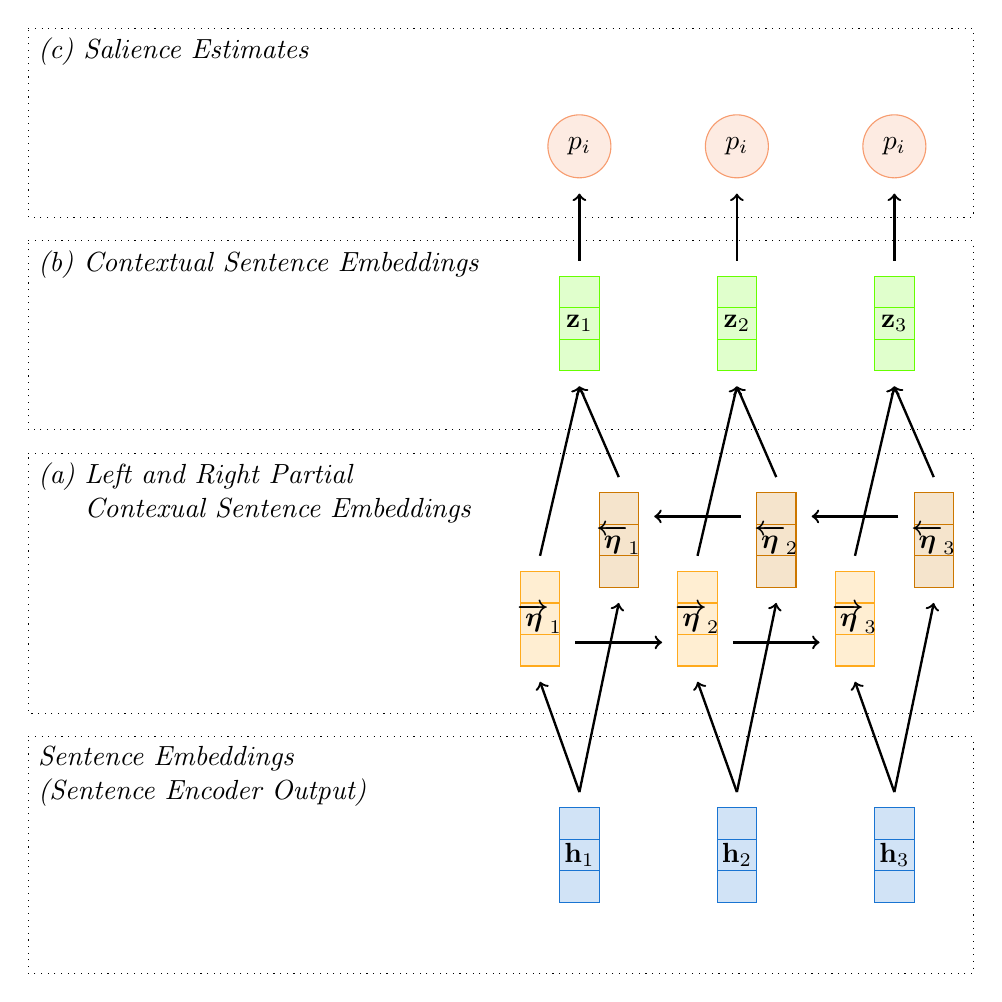
\begin{tikzpicture}[
  dep/.style ={
    ->,line width=0.3mm
  },
  hid/.style 2 args={
    rectangle split,
    draw=#2,
    rectangle split parts=#1,
    fill=#2!20,
    minimum width=5mm,
    minimum height=5mm,
    outer sep=2mm},
  mlp/.style 2 args={
    rectangle split,
    rectangle split horizontal,
    draw=#2,
    rectangle split parts=#1,
    fill=#2!20,
    outer sep=2mm},
  sal/.style={
    circle, 
    minimum width=8mm,
    outer sep=2mm,
    draw=#1, 
    fill=#1!20},
]

  \def\stepsize{2}%
  \def\lvlbase{0}%
  \def\lvlheight{3}%
 

    % Sentence Embeddings    
  \foreach \step in {1,...,3} {
    \node[hid={3}{sentemb}] (s\step) at (\stepsize*\step, \lvlbase) {};    
    \node at (\stepsize*\step, \lvlbase) {$\sentEmb_\step$};    
   }
%    \foreach \step [count=\i from 1] in {5,6} {
%        \node[hid={3}{green}] (s\step) at (\stepsize*\step, \lvlbase) {};    
%        \node at (\stepsize*\step, \lvlbase) {$\sentEmb_\i$};    
%    %\draw[->] (i\step.north) -> (e\step.south);
%    }
%
%       \node[hid={3}{red}] (s4) at (\stepsize*4, \lvlbase) {};    
%       \node at (\stepsize*4, \lvlbase) {$\sentEmb_0$};    
%
%    % RNN hidden states
    \foreach \step in {1,...,3} {
        \node[hid={3}{rencemb}] (rrnn_\step) 
            at (\stepsize *\step-0.5, \lvlbase + \lvlheight) {};    
        \node at (\stepsize *\step-0.5, \lvlbase + \lvlheight) 
            {$\rnnextRHid_\step$}; 
        \node[hid={3}{lencemb}] (lrnn_\step) 
            at (\stepsize *\step+0.5, \lvlbase + \lvlheight + 1.0) {};    
        \node at (\stepsize *\step+0.5, \lvlbase + \lvlheight+ 1.0) 
            {$\rnnextLHid_\step$}; 
        \draw[dep] (s\step.north) -- (rrnn_\step.south);
        \draw[dep] (s\step.north) -- (lrnn_\step.south);


        \node[hid={3}{ctxemb}] (ctx_\step) 
            at (\stepsize *\step, \lvlbase + 2.25*\lvlheight) {};    
        \node at (\stepsize *\step, \lvlbase + 2.25*\lvlheight) 
            {$\rnnextHid_\step$}; 
        \draw[dep] (rrnn_\step.north) -- (ctx_\step.south);
        \draw[dep] (lrnn_\step.north) -- (ctx_\step.south);


        \node[sal={sal}] (sal_\step) 
            at (\stepsize *\step, \lvlbase + 3*\lvlheight) {};    
        \node at (\stepsize *\step, \lvlbase + 3*\lvlheight) 
            {$\psal_i$}; 
        \draw[dep] (ctx_\step.north) -- (sal_\step.south);
        %\draw[dep] (lrnn_\step.north) -- (ctx_\step.south);


    }
    \foreach \start [count=\stop from 2] in {1,...,2} {
        \draw[dep] ($ (rrnn_\start.east) - (0,0.3)$) 
            -- ($ (rrnn_\stop.west) - (0,0.3) $);
        \draw[dep] ($(lrnn_\stop.west) + (0,0.3)$) 
            -- ($ (lrnn_\start.east) + (0,0.3)   $);
    }

    \draw[rectangle,draw=black,dotted] 
        (\stepsize*-2.5,\lvlbase + 3.5*\lvlheight) -- 
        (\stepsize*3.5, \lvlbase + 3.5*\lvlheight) -- 
        (\stepsize*3.5, \lvlbase + 2.7*\lvlheight) --
        (\stepsize*-2.5, \lvlbase + 2.7*\lvlheight) --
        (\stepsize*-2.5, \lvlbase + 3.5*\lvlheight) ;

    \node[align=left,anchor=north west] 
        at (\stepsize * -2.5,\lvlbase + 3.5*\lvlheight) 
        {\textit{(c) Salience Estimates}};

    \draw[rectangle,draw=black,dotted] 
        (\stepsize*-2.5,\lvlbase + 2.6*\lvlheight) -- 
        (\stepsize*3.5, \lvlbase + 2.6*\lvlheight) -- 
        (\stepsize*3.5, \lvlbase + 1.8*\lvlheight) --
        (\stepsize*-2.5, \lvlbase + 1.8*\lvlheight) --
        (\stepsize*-2.5, \lvlbase + 2.6*\lvlheight) ;

    \node[align=left,anchor=north west] 
        at (\stepsize * -2.5,\lvlbase + 2.6*\lvlheight) 
        {\textit{(b) Contextual Sentence Embeddings}};

    \draw[rectangle,draw=black,dotted] 
        (\stepsize*-2.5,\lvlbase + 0.5*\lvlheight) -- 
        (\stepsize*3.5, \lvlbase + 0.5*\lvlheight) -- 
        (\stepsize*3.5, \lvlbase + -0.50*\lvlheight) --
        (\stepsize*-2.5, \lvlbase + -0.50*\lvlheight) --
        (\stepsize*-2.5, \lvlbase + 0.5*\lvlheight) ;

    \node[align=left,anchor=north west] 
        at (\stepsize * -2.5,\lvlbase + 0.5*\lvlheight) 
        {\textit{Sentence Embeddings}\\\textit{(Sentence Encoder Output)}};


    \draw[rectangle,draw=black,dotted] 
        (\stepsize*-2.5,\lvlbase + 1.7*\lvlheight) -- 
        (\stepsize*3.5, \lvlbase + 1.7*\lvlheight) -- 
        (\stepsize*3.5, \lvlbase + 0.6*\lvlheight) --
        (\stepsize*-2.5, \lvlbase + 0.6*\lvlheight) --
        (\stepsize*-2.5, \lvlbase + 1.7*\lvlheight) ;


    \node[align=left,anchor=north west] 
        at (\stepsize * -2.5,\lvlbase + 1.7*\lvlheight) 
        {\textit{(a) Left and Right Partial}\\\textit{\phantom{(a) }Contexual Sentence Embeddings}};


\end{tikzpicture}}

\caption{Schematic for the \rnnext~sentence extractor.}
\label{fig:rnnext}
\end{minipage}}
\end{figure}

%\begin{figure}[H!]
\center
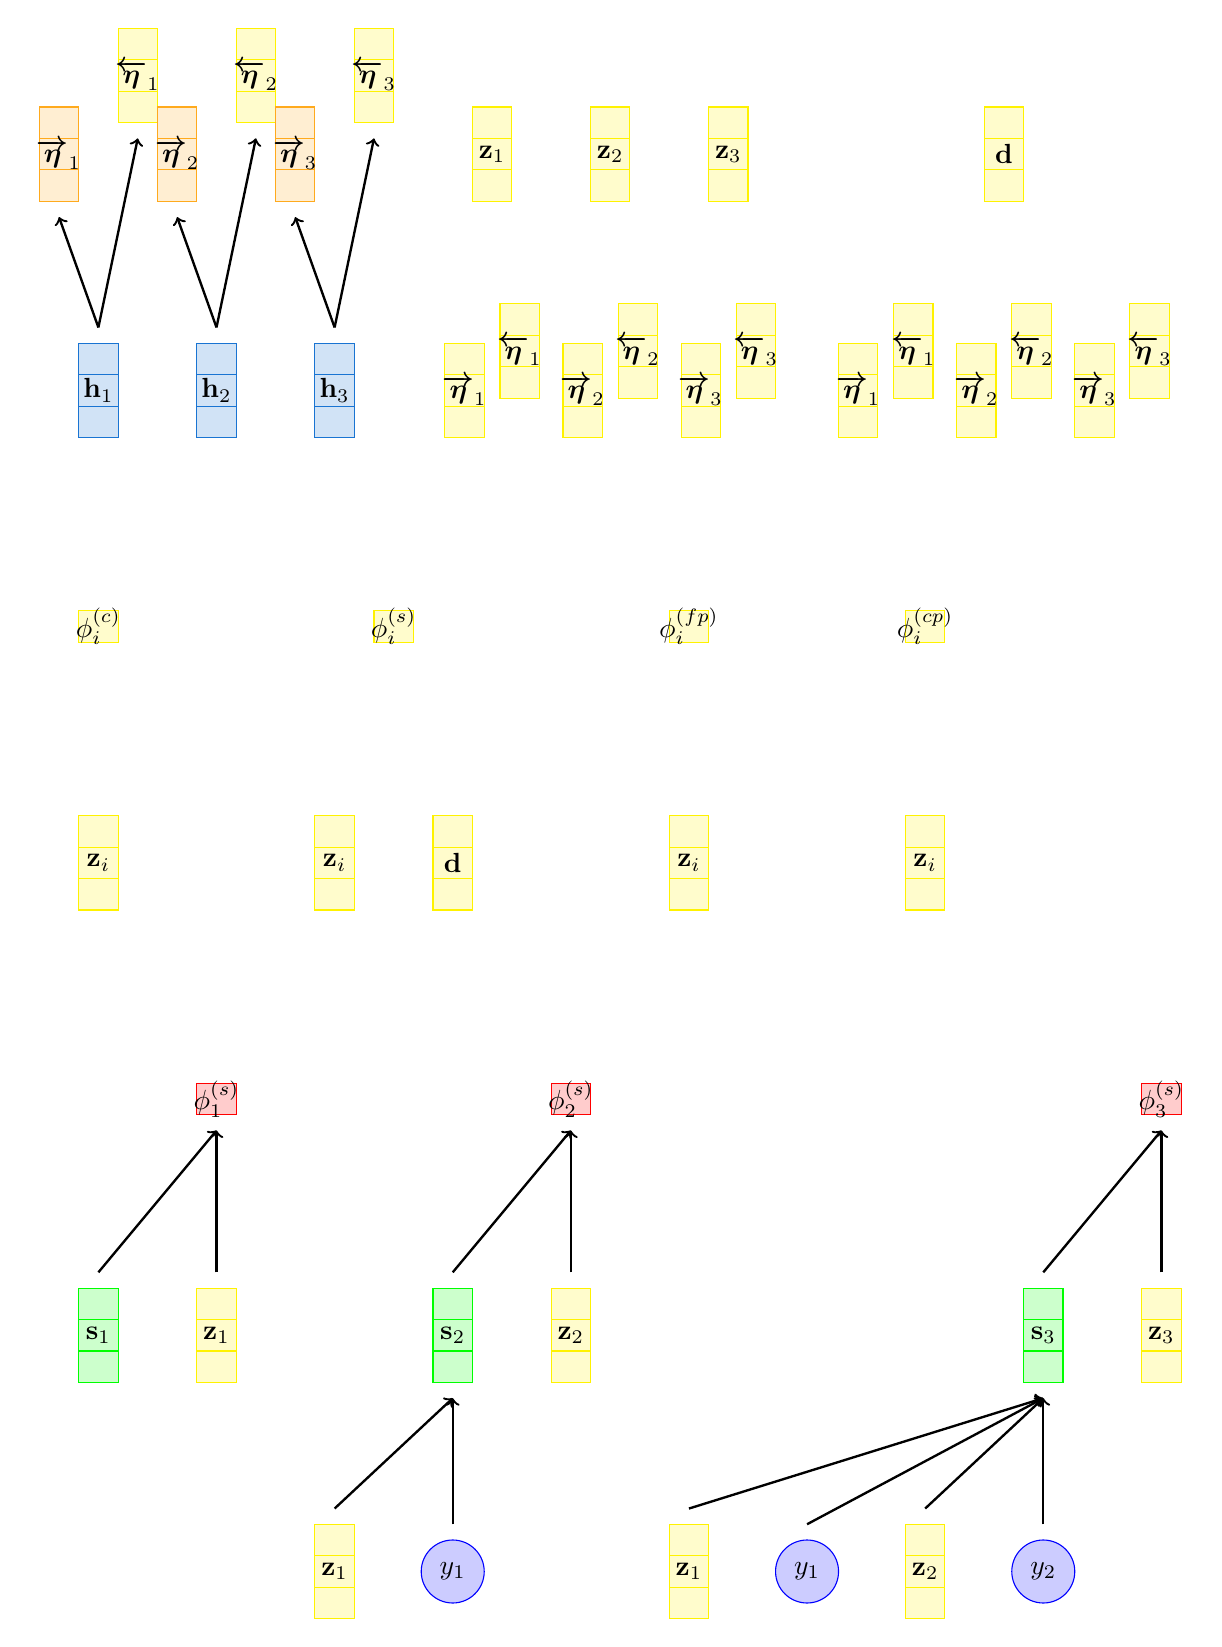
\begin{tikzpicture}[
  dep/.style ={
    ->,line width=0.3mm
  },
  hid/.style 2 args={
    rectangle split,
    draw=#2,
    rectangle split parts=#1,
    fill=#2!20,
    minimum width=5mm,
    minimum height=5mm,
    outer sep=2mm},
  mlp/.style 2 args={
    rectangle split,
    rectangle split horizontal,
    draw=#2,
    rectangle split parts=#1,
    fill=#2!20,
    outer sep=2mm},
  sal/.style={
    circle, 
    minimum width=8mm,
    outer sep=2mm,
    draw=#1, 
    fill=#1!20},
]

  \def\stepsize{1.5}%
  \def\lvlbase{0}%
  \def\lvlheight{3}%
 

    % Sentence Embeddings    
  \foreach \step in {1,...,3} {
    \node[hid={3}{sentemb}] (s\step) at (\stepsize*\step, \lvlbase) {};    
    \node at (\stepsize*\step, \lvlbase) {$\sentEmb_\step$};    
   }
%    % RNN hidden states
    \foreach \step in {1,...,3} {
        \node[hid={3}{encemb}] (rrnn_\step) 
            at (\stepsize *\step-0.5, \lvlbase + \lvlheight) {};    
        \node at (\stepsize *\step-0.5, \lvlbase + \lvlheight) 
            {$\rnnextRHid_\step$}; 
        \node[hid={3}{yellow}] (lrnn_\step) 
            at (\stepsize *\step+0.5, \lvlbase + \lvlheight + 1.0) {};    
        \node at (\stepsize *\step+0.5, \lvlbase + \lvlheight+ 1.0) 
            {$\rnnextLHid_\step$}; 
        \draw[dep] (s\step.north) -- (rrnn_\step.south);
        \draw[dep] (s\step.north) -- (lrnn_\step.south);


%        \node[hid={3}{orange}] (ctx_\step) 
%            at (\stepsize *\step, \lvlbase + 2.25*\lvlheight) {};    
%        \node at (\stepsize *\step, \lvlbase + 2.25*\lvlheight) 
%            {$\rnnextHid_\step$}; 
%        \draw[dep] (rrnn_\step.north) -- (ctx_\step.south);
%        \draw[dep] (lrnn_\step.north) -- (ctx_\step.south);
%
%
%        \node[sal={blue}] (sal_\step) 
%            at (\stepsize *\step, \lvlbase + 3*\lvlheight) {};    
%        \node at (\stepsize *\step, \lvlbase + 3*\lvlheight) 
%            {$\bsal_i$}; 
%        \draw[dep] (ctx_\step.north) -- (sal_\step.south);
        %\draw[dep] (lrnn_\step.north) -- (ctx_\step.south);


    }
  \def\stepsize{1.5}%
  \def\lvlbase{0}%
  \def\lvlheight{3}%
 

    \foreach \step in {1,...,3} {
        \node[hid={3}{yellow}] (rrnn_\step) 
            at (\stepsize *\step-0.35 + 5, \lvlbase + 0*\lvlheight) {};    
        \node at (\stepsize*\step-0.35 + 5, \lvlbase + 0*\lvlheight) 
            {$\rnnextRHid_\step$}; 
        \node[hid={3}{yellow}] (lrnn_\step) 
            at (\stepsize *\step+5.35, \lvlbase + 0*\lvlheight + 0.5) {};    
        \node at (\stepsize *\step+5.35, \lvlbase + 0*\lvlheight+ 0.5) 
            {$\rnnextLHid_\step$}; 
    }

    \foreach \step in {1,...,3} {
        \node[hid={3}{yellow}] (rrnn_\step) 
            at (\stepsize *\step-0.35 + 10, \lvlbase + 0*\lvlheight) {};    
        \node at (\stepsize*\step-0.35 + 10, \lvlbase + 0*\lvlheight) 
            {$\rnnextRHid_\step$}; 
        \node[hid={3}{yellow}] (lrnn_\step) 
            at (\stepsize *\step+10.35, \lvlbase + 0*\lvlheight + 0.5) {};    
        \node at (\stepsize *\step+10.35, \lvlbase + 0*\lvlheight+ 0.5) 
            {$\rnnextLHid_\step$}; 
    }

    \foreach \step in {1,...,3} {
        \node[hid={3}{yellow}] (ctx_\step) 
            at (\stepsize *\step + 5, \lvlbase + 1*\lvlheight) {};    
        \node at (\stepsize*\step + 5, \lvlbase + 1*\lvlheight) 
            {$\srHid_\step$}; 
    }

        \node[hid={3}{yellow}] (doc) 
            at (\stepsize *2 + 10, \lvlbase + 1*\lvlheight) {};    
        \node at (\stepsize*2 + 10, \lvlbase + 1*\lvlheight) 
            {$\srDocEmb$}; 


        \node[hid={3}{yellow}] (ctx_i) 
            at (\stepsize *1 , \lvlbase + -2*\lvlheight) {};    
        \node at (\stepsize*1, \lvlbase + -2*\lvlheight) 
            {$\srHid_i$}; 

        \node[hid={1}{yellow}] (content_i) 
            at (\stepsize *1, \lvlbase + -1*\lvlheight) {};    
        \node at (\stepsize*1, \lvlbase + -1*\lvlheight) 
            {$\srContentFactor_i$}; 

        \node[hid={3}{yellow}] (ctx_i) 
            at (\stepsize *3 , \lvlbase + -2*\lvlheight) {};    
        \node at (\stepsize*3, \lvlbase + -2*\lvlheight) 
            {$\srHid_i$}; 

        \node[hid={1}{yellow}] (salience_i) 
            at (\stepsize *3.5, \lvlbase + -1*\lvlheight) {};    
        \node at (\stepsize*3.5, \lvlbase + -1*\lvlheight) 
            {$\srSalienceFactor_i$}; 
        \node[hid={3}{yellow}] (doc) 
            at (\stepsize *4, \lvlbase + -2*\lvlheight) {};    
        \node at (\stepsize*4, \lvlbase + -2*\lvlheight) 
            {$\srDocEmb$}; 

        \node[hid={3}{yellow}] (ctx_i) 
            at (\stepsize *6 , \lvlbase + -2*\lvlheight) {};    
        \node at (\stepsize*6, \lvlbase + -2*\lvlheight) 
            {$\srHid_i$}; 

        \node[hid={1}{yellow}] (finepos_i) 
            at (\stepsize *6, \lvlbase + -1*\lvlheight) {};    
        \node at (\stepsize*6, \lvlbase + -1*\lvlheight) 
            {$\srFinePositionFactor_i$}; 

        \node[hid={3}{yellow}] (ctx_i) 
            at (\stepsize *8 , \lvlbase + -2*\lvlheight) {};    
        \node at (\stepsize*8, \lvlbase + -2*\lvlheight) 
            {$\srHid_i$}; 
        \node[hid={1}{yellow}] (coarsepos_i) 
            at (\stepsize *8, \lvlbase + -1*\lvlheight) {};    
        \node at (\stepsize*8, \lvlbase + -1*\lvlheight) 
            {$\srCoarsePositionFactor_i$}; 

    %    \node[hid={3}{yellow}] (ctx_i) 
    %        at (\stepsize *1 , \lvlbase + -5*\lvlheight) {};    
    %    \node at (\stepsize*1, \lvlbase + -5*\lvlheight) 
    %        {$\srHid_i$}; 

        \node[hid={3}{green}] (summary_1) 
            at (\stepsize *1 , \lvlbase + -4*\lvlheight) {};    
        \node at (\stepsize*1, \lvlbase + -4*\lvlheight) 
            {$\srSum_1$}; 

        \node[hid={3}{yellow}] (ctx_1) 
            at (\stepsize *2 , \lvlbase + -4*\lvlheight) {};    
        \node at (\stepsize*2, \lvlbase + -4*\lvlheight) 
            {$\srHid_1$}; 

            \node[hid={1}{red}] (salience_1) 
            at (\stepsize *2 , \lvlbase + -3*\lvlheight) {};    
        \node at (\stepsize*2, \lvlbase + -3*\lvlheight) 
            {$\srSalienceFactor_1$}; 


        \draw[dep] (summary_1.north) to (salience_1.south);
        \draw[dep] (ctx_1.north) to (salience_1.south);


        \node[hid={3}{yellow}] (ctx_1) 
            at (\stepsize *3 , \lvlbase + -5*\lvlheight) {};    
        \node at (\stepsize*3, \lvlbase + -5*\lvlheight) 
            {$\srHid_1$}; 

        \node[sal={blue}] (p_1) 
            at (\stepsize *4 , \lvlbase + -5*\lvlheight) {};    
        \node at (\stepsize*4, \lvlbase + -5*\lvlheight) 
            {$\bsal_1$}; 

        \node[hid={3}{green}] (summary_2) 
            at (\stepsize *4 , \lvlbase + -4*\lvlheight) {};    
        \node at (\stepsize*4, \lvlbase + -4*\lvlheight) 
            {$\srSum_2$}; 

        \node[hid={3}{yellow}] (ctx_2) 
            at (\stepsize *5 , \lvlbase + -4*\lvlheight) {};    
        \node at (\stepsize*5, \lvlbase + -4*\lvlheight) 
            {$\srHid_2$}; 

            \node[hid={1}{red}] (salience_2) 
            at (\stepsize *5 , \lvlbase + -3*\lvlheight) {};    
        \node at (\stepsize*5, \lvlbase + -3*\lvlheight) 
            {$\srSalienceFactor_2$}; 


        \draw[dep] (summary_2.north) to (salience_2.south);
        \draw[dep] (ctx_2.north) to (salience_2.south);


        \draw[dep] (ctx_1.north) to (summary_2.south);
        \draw[dep] (p_1.north) to (summary_2.south);








        \node[hid={3}{yellow}] (ctx_1) 
            at (\stepsize *6 , \lvlbase + -5*\lvlheight) {};    
        \node at (\stepsize*6, \lvlbase + -5*\lvlheight) 
            {$\srHid_1$}; 

        \node[sal={blue}] (p_1) 
            at (\stepsize *7 , \lvlbase + -5*\lvlheight) {};    
        \node at (\stepsize*7, \lvlbase + -5*\lvlheight) 
            {$\bsal_1$}; 

        \node[hid={3}{yellow}] (ctx_2) 
            at (\stepsize *8 , \lvlbase + -5*\lvlheight) {};    
        \node at (\stepsize*8, \lvlbase + -5*\lvlheight) 
            {$\srHid_2$}; 

        \node[sal={blue}] (p_2) 
            at (\stepsize *9 , \lvlbase + -5*\lvlheight) {};    
        \node at (\stepsize*9, \lvlbase + -5*\lvlheight) 
            {$\bsal_2$}; 



        \node[hid={3}{green}] (summary_3) 
            at (\stepsize *9 , \lvlbase + -4*\lvlheight) {};    
        \node at (\stepsize*9, \lvlbase + -4*\lvlheight) 
            {$\srSum_3$}; 

        \node[hid={3}{yellow}] (ctx_3) 
            at (\stepsize *10 , \lvlbase + -4*\lvlheight) {};    
        \node at (\stepsize*10, \lvlbase + -4*\lvlheight) 
            {$\srHid_3$}; 

            \node[hid={1}{red}] (salience_3) 
            at (\stepsize *10 , \lvlbase + -3*\lvlheight) {};    
        \node at (\stepsize*10, \lvlbase + -3*\lvlheight) 
            {$\srSalienceFactor_3$}; 


        \draw[dep] (ctx_1.north) to (summary_3.south);
        \draw[dep] (p_1.north) to (summary_3.south);

        \draw[dep] (ctx_2.north) to (summary_3.south);
        \draw[dep] (p_2.north) to (summary_3.south);

        \draw[dep] (summary_3.north) to (salience_3.south);
        \draw[dep] (ctx_3.north) to (salience_3.south);













%        \node[hid={3}{yellow}] (ctx_1) 
%            at (\stepsize *4 , \lvlbase + -5*\lvlheight) {};    
%        \node at (\stepsize*4, \lvlbase + -5*\lvlheight) 
%            {$\srHid_1$}; 
%        \node[hid={3}{yellow}] (ctx_2) 
%            at (\stepsize *5 , \lvlbase + -5*\lvlheight) {};    
%        \node at (\stepsize*5, \lvlbase + -5*\lvlheight) 
%            {$\srHid_2$}; 
%
%
%

%    \foreach \start [count=\stop from 2] in {1,...,2} {
%        \draw[dep] ($ (rrnn_\start.east) - (0,0.3)$) 
%            -- ($ (rrnn_\stop.west) - (0,0.3) $);
%        \draw[dep] ($(lrnn_\stop.west) + (0,0.3)$) 
%            -- ($ (lrnn_\start.east) + (0,0.3)   $);
%    }

%    \draw[rectangle,draw=black,dotted] 
%        (\stepsize*-2.5,\lvlbase + 3.5*\lvlheight) -- 
%        (\stepsize*3.5, \lvlbase + 3.5*\lvlheight) -- 
%        (\stepsize*3.5, \lvlbase + 2.7*\lvlheight) --
%        (\stepsize*-2.5, \lvlbase + 2.7*\lvlheight) --
%        (\stepsize*-2.5, \lvlbase + 3.5*\lvlheight) ;
%
%    \node[align=left,anchor=north west] 
%        at (\stepsize * -2.5,\lvlbase + 3.5*\lvlheight) 
%        {\textit{Salience Estimates}};
%
%    \draw[rectangle,draw=black,dotted] 
%        (\stepsize*-2.5,\lvlbase + 2.6*\lvlheight) -- 
%        (\stepsize*3.5, \lvlbase + 2.6*\lvlheight) -- 
%        (\stepsize*3.5, \lvlbase + 1.8*\lvlheight) --
%        (\stepsize*-2.5, \lvlbase + 1.8*\lvlheight) --
%        (\stepsize*-2.5, \lvlbase + 2.6*\lvlheight) ;
%
%    \node[align=left,anchor=north west] 
%        at (\stepsize * -2.5,\lvlbase + 2.6*\lvlheight) 
%        {\textit{Contextual Sentence Embeddings}};
%
%    \draw[rectangle,draw=black,dotted] 
%        (\stepsize*-2.5,\lvlbase + 0.5*\lvlheight) -- 
%        (\stepsize*3.5, \lvlbase + 0.5*\lvlheight) -- 
%        (\stepsize*3.5, \lvlbase + -0.50*\lvlheight) --
%        (\stepsize*-2.5, \lvlbase + -0.50*\lvlheight) --
%        (\stepsize*-2.5, \lvlbase + 0.5*\lvlheight) ;
%
%    \node[align=left,anchor=north west] 
%        at (\stepsize * -2.5,\lvlbase + 0.5*\lvlheight) 
%        {\textit{Sentence Embeddings}\\\textit{(Sentence Encoder Output)}};
%
%
%    \draw[rectangle,draw=black,dotted] 
%        (\stepsize*-2.5,\lvlbase + 1.7*\lvlheight) -- 
%        (\stepsize*3.5, \lvlbase + 1.7*\lvlheight) -- 
%        (\stepsize*3.5, \lvlbase + 0.6*\lvlheight) --
%        (\stepsize*-2.5, \lvlbase + 0.6*\lvlheight) --
%        (\stepsize*-2.5, \lvlbase + 1.7*\lvlheight) ;
%
%
%    \node[align=left,anchor=north west] 
%        at (\stepsize * -2.5,\lvlbase + 1.7*\lvlheight) 
%        {\textit{Forward and Backward Partial}\\\textit{Contexual Sentence Embeddings}};


\end{tikzpicture}


\end{figure}

%\begin{figure}[H!]
\center
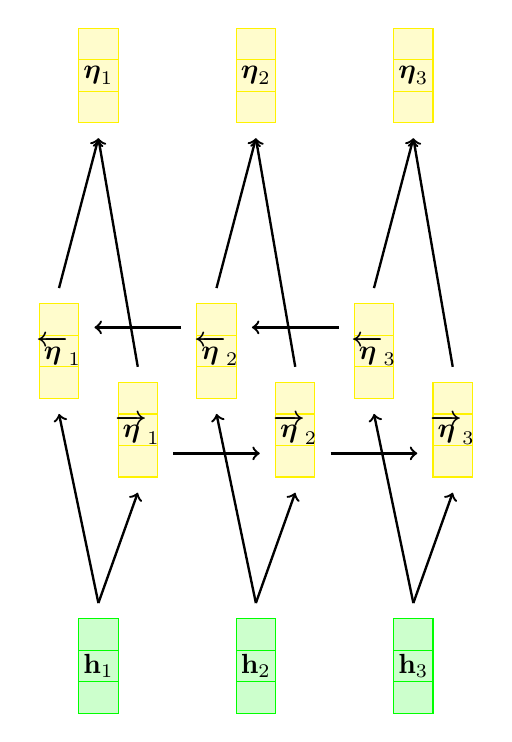
\begin{tikzpicture}[
  dep/.style ={
    ->,line width=0.3mm
  },
  hid/.style 2 args={
    rectangle split,
    draw=#2,
    rectangle split parts=#1,
    fill=#2!20,
    minimum width=5mm,
    minimum height=5mm,
    outer sep=2mm},
  mlp/.style 2 args={
    rectangle split,
    rectangle split horizontal,
    draw=#2,
    rectangle split parts=#1,
    fill=#2!20,
    outer sep=2mm},
  sal/.style={
    circle, 
    minimum width=8mm,
    outer sep=2mm,
    draw=#1, 
    fill=#1!20},
]

  \def\stepsize{2}%
  \def\lvlbase{0}%
  \def\lvlheight{3}%
 

    % Sentence Embeddings    
  \foreach \step in {1,...,3} {
    \node[hid={3}{green}] (s\step) at (\stepsize*\step, \lvlbase) {};    
    \node at (\stepsize*\step, \lvlbase) {$\sentEmb_\step$};    
   }
%    \foreach \step [count=\i from 1] in {5,...,7} {
%        \node[hid={3}{green}] (s\step) at (\stepsize*\step, \lvlbase) {};    
%        \node at (\stepsize*\step, \lvlbase) {$\sentEmb_\i$};    
%    %\draw[->] (i\step.north) -> (e\step.south);
%    }

%       \node[hid={3}{red}] (s4) at (\stepsize*4, \lvlbase) {};    
%       \node at (\stepsize*4, \lvlbase) {$\sentEmb_0$};    
%
%    % RNN hidden states
    \foreach \step in {1,...,3} {
        \node[hid={3}{yellow}] (rrnn_\step) 
            at (\stepsize *\step+0.5, \lvlbase + \lvlheight) {};    
        \node at (\stepsize *\step+0.5, \lvlbase + \lvlheight) 
            {$\stsextREncHid_\step$}; 

        \node[hid={3}{yellow}] (lrnn_\step) 
            at (\stepsize *\step-0.5, \lvlbase + \lvlheight+1.0) {};    
        \node at (\stepsize *\step-0.5, \lvlbase + \lvlheight+1.0) 
            {$\stsextLEncHid_\step$}; 


        \node[hid={3}{yellow}] (enc_ctx_\step) 
            at (\stepsize *\step, \lvlbase + 2.5*\lvlheight) {};    
        \node at (\stepsize *\step, \lvlbase + 2.5*\lvlheight) 
            {$\stsextEncHid_\step$}; 

        \draw[dep] (s\step.north) -- (lrnn_\step.south);
        \draw[dep] (s\step.north) -- (rrnn_\step.south);

        \draw[dep] (lrnn_\step.north) -- (enc_ctx_\step.south);
        \draw[dep] (rrnn_\step.north) -- (enc_ctx_\step.south);
    }
    \foreach \start [count=\stop from 2] in {1,...,2} {
        \draw[dep] ($ (rrnn_\start.east) - (0,0.3)$) 
            -- ($ (rrnn_\stop.west) - (0,0.3) $);
        \draw[dep] ($(lrnn_\stop.west) + (0,0.3)$) 
            -- ($ (lrnn_\start.east) + (0,0.3)   $);
    }




%    \foreach \step [count=\i from 0] in {4,...,7} {
%        \node[hid={3}{orange}] (rnn_\step) 
%            at (\stepsize *\step, \lvlbase + \lvlheight) {};    
%        \node at (\stepsize *\step, \lvlbase + \lvlheight) {$\xDecHid_\i$}; 
%    }
%
%    \foreach \step in {1,...,6} {
%        \draw[dep] (s\step.north) to (rnn_\step.south);
%    }
%    \foreach \start [count=\stop from 2] in {1,...,5} {
%        \draw[dep] (rnn_\start.east) to (rnn_\stop.west);
%    }
%
%
%%    \foreach \step [count=\i from 1] in {4,...,6} {
%%        \node[hid={3}{green}] (ctx_\i) 
%%            at (\stepsize *\step, \lvlbase + 2*\lvlheight) {};    
%%        \node at (\stepsize *\step, \lvlbase + 2*\lvlheight) {$\xPredHid_\i$}; 
%%        \draw[dep] (rnn_\step.north) to (ctx_\i.south);
%%        \draw[dep] (rnn_\i.north) to (ctx_\i.south west);
%%        \node[sal={blue}] (sal_\i) at (\stepsize * \step,\lvlbase + 3*\lvlheight) {};
%%        \node at (\stepsize * \step,\lvlbase + 3*\lvlheight) {$\bsal_\i$};
%%        \draw[dep] (ctx_\i.north) to (sal_\i.south);
%%    }
%%
%%    \foreach \step [count=\i from 1] in {5,...,6} {
%%        \draw[dep] (sal_\i) -- (\stepsize * \step - \stepsize / 2,
%%                            \lvlbase + 3*\lvlheight) 
%%                     -- (\stepsize * \step - \stepsize / 2,
%%                            \lvlbase + 0* \lvlheight) -> (s\step) ;
%%
%%    }
%%    \draw[dep] (s1.south) -- ($ (s1.south) + (0,-0.3)$) --($ (s5.south) + (0,-0.3)$) -- (s5.south);
%%
%%    \draw[dep] (s2.south) -- ($ (s2.south) + (0,-0.5)$) --($ (s6.south) + (0,-0.5)$) -- (s6.south);
%%
%%    \draw[rectangle,draw=black,dotted] 
%%        (\stepsize * 3.5,\lvlbase + 3.5*\lvlheight) -- 
%%        (\stepsize*6.5, \lvlbase + 3.5*\lvlheight) -- 
%%        (\stepsize*6.5, \lvlbase + 2.6*\lvlheight) --
%%        (\stepsize*3.5, \lvlbase + 2.6*\lvlheight) --
%%        (\stepsize*3.5, \lvlbase + 3.5*\lvlheight) ;
%%
%%    \node[align=left,anchor=north west] 
%%        at (\stepsize * 3.5,\lvlbase + 3.5*\lvlheight) 
%%        {\textit{Salience Estimates}};
%%
%%    \draw[rectangle,draw=black,dotted] 
%%        (\stepsize*0.5,\lvlbase + 2.5*\lvlheight) -- 
%%        (\stepsize*6.5, \lvlbase + 2.5*\lvlheight) -- 
%%        (\stepsize*6.5, \lvlbase + 1.5*\lvlheight) --
%%        (\stepsize*0.5, \lvlbase + 1.5*\lvlheight) --
%%        (\stepsize*0.5, \lvlbase + 2.5*\lvlheight) ;
%%
%%    \node[align=left,anchor=north west] 
%%        at (\stepsize * 0.5,\lvlbase + 2.5*\lvlheight) 
%%        {\textit{Contextual Sentence Embeddings}};
%%
%%    \draw[rectangle,draw=black,dotted] 
%%        (\stepsize*-0.5,\lvlbase + 0.5*\lvlheight) -- 
%%        (\stepsize*3.5, \lvlbase + 0.5*\lvlheight) -- 
%%        (\stepsize*3.5, \lvlbase + -0.9*\lvlheight) --
%%        (\stepsize*-0.5, \lvlbase + -0.9*\lvlheight) --
%%        (\stepsize*-0.5, \lvlbase + 0.5*\lvlheight) ;
%%
%%    \node[align=left,anchor=south west] 
%%        at (\stepsize * -0.5,\lvlbase + -0.9*\lvlheight) 
%%        {\textit{Sentence Embeddings}\\\textit{(Sentence Encoder Output)}};
%%
%%    \draw[rectangle,draw=black,dotted] 
%%        (\stepsize*4.3,\lvlbase + 0.5*\lvlheight) -- 
%%        (\stepsize*6.5, \lvlbase + 0.5*\lvlheight) -- 
%%        (\stepsize*6.5, \lvlbase + -0.9*\lvlheight) --
%%        (\stepsize*4.3, \lvlbase + -0.9*\lvlheight) --
%%        (\stepsize*4.3, \lvlbase + 0.5*\lvlheight) ;
%%
%%    \node[align=left,anchor=south west] 
%%        at (\stepsize * 4.3,\lvlbase + -0.9*\lvlheight) 
%%        {\textit{Salience Gated}\\\textit{Sentence Embeddings}};
%%

    



\end{tikzpicture}

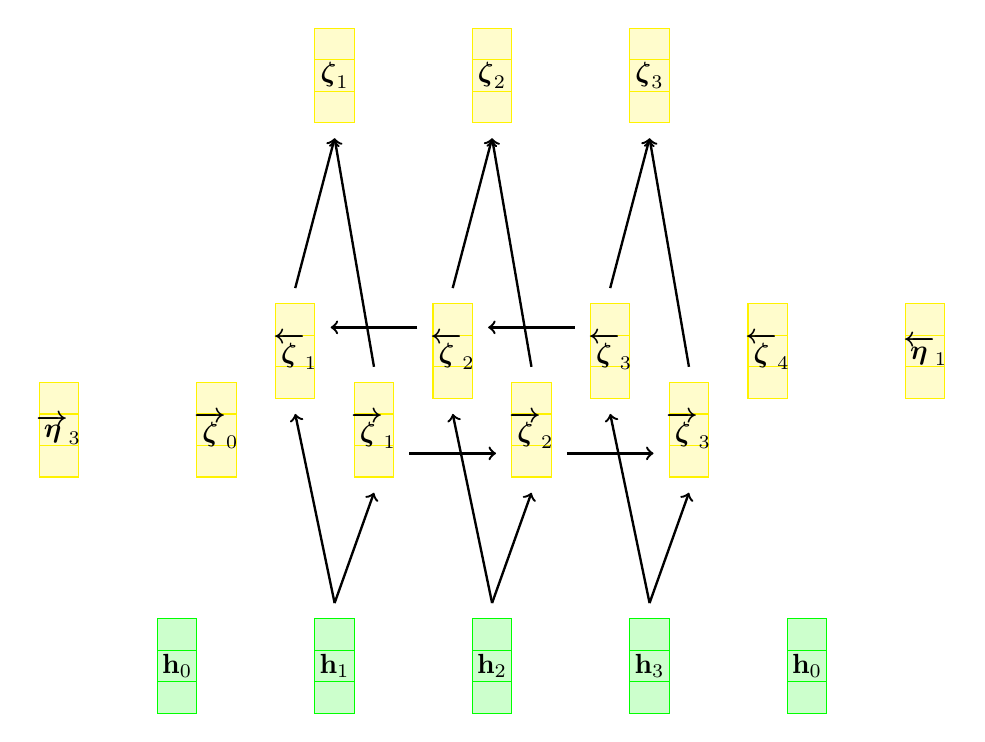
\begin{tikzpicture}[
  dep/.style ={
    ->,line width=0.3mm
  },
  hid/.style 2 args={
    rectangle split,
    draw=#2,
    rectangle split parts=#1,
    fill=#2!20,
    minimum width=5mm,
    minimum height=5mm,
    outer sep=2mm},
  mlp/.style 2 args={
    rectangle split,
    rectangle split horizontal,
    draw=#2,
    rectangle split parts=#1,
    fill=#2!20,
    outer sep=2mm},
  sal/.style={
    circle, 
    minimum width=8mm,
    outer sep=2mm,
    draw=#1, 
    fill=#1!20},
]

  \def\stepsize{2}%
  \def\lvlbase{0}%
  \def\lvlheight{3}%
 

    \node[hid={3}{green}] (s0) at (\stepsize*0, \lvlbase) {};    
    \node at (\stepsize*0, \lvlbase) {$\sentEmb_0$};    


    \node[hid={3}{green}] (s4) at (\stepsize*4, \lvlbase) {};    
    \node at (\stepsize*4, \lvlbase) {$\sentEmb_0$};    

    % Sentence Embeddings    
  \foreach \step in {1,...,3} {
    \node[hid={3}{green}] (s\step) at (\stepsize*\step, \lvlbase) {};    
    \node at (\stepsize*\step, \lvlbase) {$\sentEmb_\step$};    
   }
%    \foreach \step [count=\i from 1] in {5,...,7} {
%        \node[hid={3}{green}] (s\step) at (\stepsize*\step, \lvlbase) {};    
%        \node at (\stepsize*\step, \lvlbase) {$\sentEmb_\i$};    
%    %\draw[->] (i\step.north) -> (e\step.south);
%    }

%       \node[hid={3}{red}] (s4) at (\stepsize*4, \lvlbase) {};    
%       \node at (\stepsize*4, \lvlbase) {$\sentEmb_0$};    
%
%    % RNN hidden states

        \node[hid={3}{yellow}] (rrnn_0) 
            at (\stepsize *0+0.5, \lvlbase + \lvlheight) {};    
        \node at (\stepsize *0+0.5, \lvlbase + \lvlheight) 
            {$\stsextRDecHid_0$}; 

        \node[hid={3}{yellow}] (lrnn_4) 
            at (\stepsize *4-0.5, \lvlbase + \lvlheight+1.0) {};    
        \node at (\stepsize *4-0.5, \lvlbase + \lvlheight+1.0) 
            {$\stsextLDecHid_4$}; 

        \node[hid={3}{yellow}] (rrnn_m1) 
            at (-\stepsize +0.5, \lvlbase + \lvlheight) {};    
        \node at (-\stepsize +0.5, \lvlbase + \lvlheight) 
            {$\stsextREncHid_3$}; 

        \node[hid={3}{yellow}] (lrnn_m1) 
            at (\stepsize*5 -0.5, \lvlbase + \lvlheight+1.0) {};    
        \node at (\stepsize*5 -0.5, \lvlbase + \lvlheight+1.0) 
            {$\stsextLEncHid_1$}; 



    \foreach \step in {1,...,3} {
        \node[hid={3}{yellow}] (rrnn_\step) 
            at (\stepsize *\step+0.5, \lvlbase + \lvlheight) {};    
        \node at (\stepsize *\step+0.5, \lvlbase + \lvlheight) 
            {$\stsextRDecHid_\step$}; 

        \node[hid={3}{yellow}] (lrnn_\step) 
            at (\stepsize *\step-0.5, \lvlbase + \lvlheight+1.0) {};    
        \node at (\stepsize *\step-0.5, \lvlbase + \lvlheight+1.0) 
            {$\stsextLDecHid_\step$}; 


        \node[hid={3}{yellow}] (enc_ctx_\step) 
            at (\stepsize *\step, \lvlbase + 2.5*\lvlheight) {};    
        \node at (\stepsize *\step, \lvlbase + 2.5*\lvlheight) 
            {$\stsextDecHid_\step$}; 

        \draw[dep] (s\step.north) -- (lrnn_\step.south);
        \draw[dep] (s\step.north) -- (rrnn_\step.south);

        \draw[dep] (lrnn_\step.north) -- (enc_ctx_\step.south);
        \draw[dep] (rrnn_\step.north) -- (enc_ctx_\step.south);
    }
    \foreach \start [count=\stop from 2] in {1,...,2} {
        \draw[dep] ($ (rrnn_\start.east) - (0,0.3)$) 
            -- ($ (rrnn_\stop.west) - (0,0.3) $);
        \draw[dep] ($(lrnn_\stop.west) + (0,0.3)$) 
            -- ($ (lrnn_\start.east) + (0,0.3)   $);
    }




%    \foreach \step [count=\i from 0] in {4,...,7} {
%        \node[hid={3}{orange}] (rnn_\step) 
%            at (\stepsize *\step, \lvlbase + \lvlheight) {};    
%        \node at (\stepsize *\step, \lvlbase + \lvlheight) {$\xDecHid_\i$}; 
%    }
%
%    \foreach \step in {1,...,6} {
%        \draw[dep] (s\step.north) to (rnn_\step.south);
%    }
%    \foreach \start [count=\stop from 2] in {1,...,5} {
%        \draw[dep] (rnn_\start.east) to (rnn_\stop.west);
%    }
%
%
%%    \foreach \step [count=\i from 1] in {4,...,6} {
%%        \node[hid={3}{green}] (ctx_\i) 
%%            at (\stepsize *\step, \lvlbase + 2*\lvlheight) {};    
%%        \node at (\stepsize *\step, \lvlbase + 2*\lvlheight) {$\xPredHid_\i$}; 
%%        \draw[dep] (rnn_\step.north) to (ctx_\i.south);
%%        \draw[dep] (rnn_\i.north) to (ctx_\i.south west);
%%        \node[sal={blue}] (sal_\i) at (\stepsize * \step,\lvlbase + 3*\lvlheight) {};
%%        \node at (\stepsize * \step,\lvlbase + 3*\lvlheight) {$\bsal_\i$};
%%        \draw[dep] (ctx_\i.north) to (sal_\i.south);
%%    }
%%
%%    \foreach \step [count=\i from 1] in {5,...,6} {
%%        \draw[dep] (sal_\i) -- (\stepsize * \step - \stepsize / 2,
%%                            \lvlbase + 3*\lvlheight) 
%%                     -- (\stepsize * \step - \stepsize / 2,
%%                            \lvlbase + 0* \lvlheight) -> (s\step) ;
%%
%%    }
%%    \draw[dep] (s1.south) -- ($ (s1.south) + (0,-0.3)$) --($ (s5.south) + (0,-0.3)$) -- (s5.south);
%%
%%    \draw[dep] (s2.south) -- ($ (s2.south) + (0,-0.5)$) --($ (s6.south) + (0,-0.5)$) -- (s6.south);
%%
%%    \draw[rectangle,draw=black,dotted] 
%%        (\stepsize * 3.5,\lvlbase + 3.5*\lvlheight) -- 
%%        (\stepsize*6.5, \lvlbase + 3.5*\lvlheight) -- 
%%        (\stepsize*6.5, \lvlbase + 2.6*\lvlheight) --
%%        (\stepsize*3.5, \lvlbase + 2.6*\lvlheight) --
%%        (\stepsize*3.5, \lvlbase + 3.5*\lvlheight) ;
%%
%%    \node[align=left,anchor=north west] 
%%        at (\stepsize * 3.5,\lvlbase + 3.5*\lvlheight) 
%%        {\textit{Salience Estimates}};
%%
%%    \draw[rectangle,draw=black,dotted] 
%%        (\stepsize*0.5,\lvlbase + 2.5*\lvlheight) -- 
%%        (\stepsize*6.5, \lvlbase + 2.5*\lvlheight) -- 
%%        (\stepsize*6.5, \lvlbase + 1.5*\lvlheight) --
%%        (\stepsize*0.5, \lvlbase + 1.5*\lvlheight) --
%%        (\stepsize*0.5, \lvlbase + 2.5*\lvlheight) ;
%%
%%    \node[align=left,anchor=north west] 
%%        at (\stepsize * 0.5,\lvlbase + 2.5*\lvlheight) 
%%        {\textit{Contextual Sentence Embeddings}};
%%
%%    \draw[rectangle,draw=black,dotted] 
%%        (\stepsize*-0.5,\lvlbase + 0.5*\lvlheight) -- 
%%        (\stepsize*3.5, \lvlbase + 0.5*\lvlheight) -- 
%%        (\stepsize*3.5, \lvlbase + -0.9*\lvlheight) --
%%        (\stepsize*-0.5, \lvlbase + -0.9*\lvlheight) --
%%        (\stepsize*-0.5, \lvlbase + 0.5*\lvlheight) ;
%%
%%    \node[align=left,anchor=south west] 
%%        at (\stepsize * -0.5,\lvlbase + -0.9*\lvlheight) 
%%        {\textit{Sentence Embeddings}\\\textit{(Sentence Encoder Output)}};
%%
%%    \draw[rectangle,draw=black,dotted] 
%%        (\stepsize*4.3,\lvlbase + 0.5*\lvlheight) -- 
%%        (\stepsize*6.5, \lvlbase + 0.5*\lvlheight) -- 
%%        (\stepsize*6.5, \lvlbase + -0.9*\lvlheight) --
%%        (\stepsize*4.3, \lvlbase + -0.9*\lvlheight) --
%%        (\stepsize*4.3, \lvlbase + 0.5*\lvlheight) ;
%%
%%    \node[align=left,anchor=south west] 
%%        at (\stepsize * 4.3,\lvlbase + -0.9*\lvlheight) 
%%        {\textit{Salience Gated}\\\textit{Sentence Embeddings}};
%%

    



\end{tikzpicture}



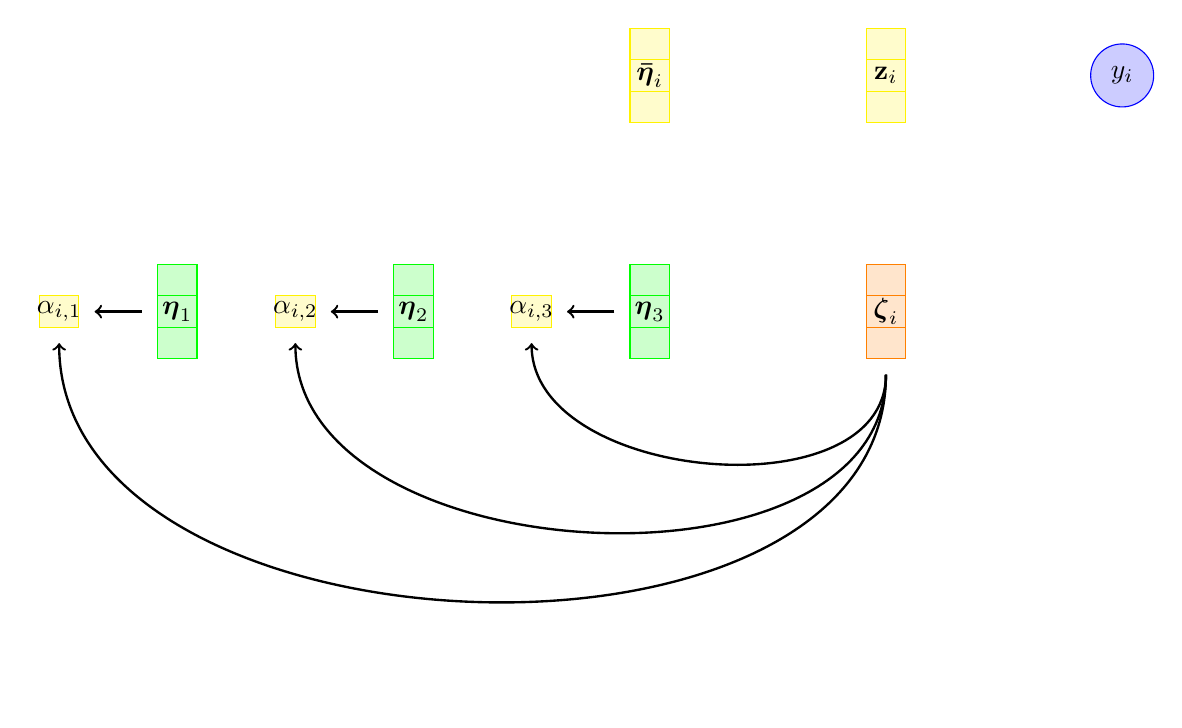
\begin{tikzpicture}[
  dep/.style ={
    ->,line width=0.3mm
  },
  hid/.style 2 args={
    rectangle split,
    draw=#2,
    rectangle split parts=#1,
    fill=#2!20,
    minimum width=5mm,
    minimum height=5mm,
    outer sep=2mm},
  mlp/.style 2 args={
    rectangle split,
    rectangle split horizontal,
    draw=#2,
    rectangle split parts=#1,
    fill=#2!20,
    outer sep=2mm},
  sal/.style={
    circle, 
    minimum width=8mm,
    outer sep=2mm,
    draw=#1, 
    fill=#1!20},
]

  \def\stepsize{3}%
  \def\lvlbase{0}%
  \def\lvlheight{3}%
 


    % Sentence Embeddings    
  \foreach \step in {1,...,3} {
    \node[hid={3}{green}] (enc\step) at (\stepsize*\step, \lvlbase) {};    
    \node at (\stepsize*\step, \lvlbase) {$\stsextEncHid_\step$};    
   }

  \foreach \step in {1,...,3} {
    \node[hid={1}{yellow}] (a\step) at (\stepsize*\step-0.5*\stepsize, \lvlbase) {};    
    \node at (\stepsize*\step-0.5*\stepsize, \lvlbase) {$\stsextAttn_{i,\step}$};    

    \draw[dep] (enc\step.west) to (a\step.east);
   }


    \node[hid={3}{orange}] (deci) at (\stepsize*4, \lvlbase) {};    
    \node at (\stepsize*4, \lvlbase) {$\stsextDecHid_i$};    

    \draw[dep] (deci.south) to [out=270,in=270] (a3.south);
    \draw[dep] (deci.south) to [out=270,in=270] (a2.south);
    \draw[dep] (deci.south) to [out=270,in=270] (a1.south);

    \node[hid={3}{yellow}] (encattn) at (\stepsize*3, \lvlbase+\lvlheight) {};    
    \node at (\stepsize*3, \lvlbase+\lvlheight) {$\stsextAttnHid_i$};    


    \node[hid={3}{yellow}] (encattn) at (\stepsize*4, \lvlbase+\lvlheight) {};    
    \node at (\stepsize*4, \lvlbase+\lvlheight) {$\stsextHid_i$};    

        \node[sal={blue}] at (\stepsize * 5,\lvlbase + \lvlheight) {};
        \node at (\stepsize * 5,\lvlbase + \lvlheight) {$\bsal_i$};
%  \foreach \step [count=\i from 1] in {4,...,6} {
%    \node[hid={3}{green}] (s\i) at (\stepsize*\step-0.5*\stepsize, \lvlbase) {};    
%    \node at (\stepsize*\step-0.5*\stepsize, \lvlbase) {$\stsextDecHid_\i$};    
%   }
%
%  \foreach \step [count=\i from 1]  in {2,...,4} {
%    \node[hid={3}{green}] (s\i) at (\stepsize*\step, \lvlbase+\lvlheight) {};    
%    \node at (\stepsize*\step, \lvlbase+\lvlheight) {$\stsextAttnHid_\i$};    
%   }
%



%    \foreach \step [count=\i from 1] in {5,...,7} {
%        \node[hid={3}{green}] (s\step) at (\stepsize*\step, \lvlbase) {};    
%        \node at (\stepsize*\step, \lvlbase) {$\sentEmb_\i$};    
%    %\draw[->] (i\step.north) -> (e\step.south);
%    }

%       \node[hid={3}{red}] (s4) at (\stepsize*4, \lvlbase) {};    
%       \node at (\stepsize*4, \lvlbase) {$\sentEmb_0$};    
%
%    % RNN hidden states

%        \node[hid={3}{yellow}] (rrnn_0) 
%            at (\stepsize *0+0.5, \lvlbase + \lvlheight) {};    
%        \node at (\stepsize *0+0.5, \lvlbase + \lvlheight) 
%            {$\stsextRDecHid_0$}; 
%
%        \node[hid={3}{yellow}] (lrnn_4) 
%            at (\stepsize *4-0.5, \lvlbase + \lvlheight+1.0) {};    
%        \node at (\stepsize *4-0.5, \lvlbase + \lvlheight+1.0) 
%            {$\stsextLDecHid_4$}; 
%
%        \node[hid={3}{yellow}] (rrnn_m1) 
%            at (-\stepsize +0.5, \lvlbase + \lvlheight) {};    
%        \node at (-\stepsize +0.5, \lvlbase + \lvlheight) 
%            {$\stsextREncHid_3$}; 
%
%        \node[hid={3}{yellow}] (lrnn_m1) 
%            at (\stepsize*5 -0.5, \lvlbase + \lvlheight+1.0) {};    
%        \node at (\stepsize*5 -0.5, \lvlbase + \lvlheight+1.0) 
%            {$\stsextLEncHid_1$}; 
%
%
%
%    \foreach \step in {1,...,3} {
%        \node[hid={3}{yellow}] (rrnn_\step) 
%            at (\stepsize *\step+0.5, \lvlbase + \lvlheight) {};    
%        \node at (\stepsize *\step+0.5, \lvlbase + \lvlheight) 
%            {$\stsextRDecHid_\step$}; 
%
%        \node[hid={3}{yellow}] (lrnn_\step) 
%            at (\stepsize *\step-0.5, \lvlbase + \lvlheight+1.0) {};    
%        \node at (\stepsize *\step-0.5, \lvlbase + \lvlheight+1.0) 
%            {$\stsextLDecHid_\step$}; 
%
%
%        \node[hid={3}{yellow}] (enc_ctx_\step) 
%            at (\stepsize *\step, \lvlbase + 2.5*\lvlheight) {};    
%        \node at (\stepsize *\step, \lvlbase + 2.5*\lvlheight) 
%            {$\stsextDecHid_\step$}; 
%
%        \draw[dep] (s\step.north) -- (lrnn_\step.south);
%        \draw[dep] (s\step.north) -- (rrnn_\step.south);
%
%        \draw[dep] (lrnn_\step.north) -- (enc_ctx_\step.south);
%        \draw[dep] (rrnn_\step.north) -- (enc_ctx_\step.south);
%    }
%    \foreach \start [count=\stop from 2] in {1,...,2} {
%        \draw[dep] ($ (rrnn_\start.east) - (0,0.3)$) 
%            -- ($ (rrnn_\stop.west) - (0,0.3) $);
%        \draw[dep] ($(lrnn_\stop.west) + (0,0.3)$) 
%            -- ($ (lrnn_\start.east) + (0,0.3)   $);
%    }
%
%
%
%
%%    \foreach \step [count=\i from 0] in {4,...,7} {
%%        \node[hid={3}{orange}] (rnn_\step) 
%%            at (\stepsize *\step, \lvlbase + \lvlheight) {};    
%%        \node at (\stepsize *\step, \lvlbase + \lvlheight) {$\xDecHid_\i$}; 
%%    }
%%
%%    \foreach \step in {1,...,6} {
%%        \draw[dep] (s\step.north) to (rnn_\step.south);
%%    }
%%    \foreach \start [count=\stop from 2] in {1,...,5} {
%%        \draw[dep] (rnn_\start.east) to (rnn_\stop.west);
%%    }
%%
%%
%%%    \foreach \step [count=\i from 1] in {4,...,6} {
%%%        \node[hid={3}{green}] (ctx_\i) 
%%%            at (\stepsize *\step, \lvlbase + 2*\lvlheight) {};    
%%%        \node at (\stepsize *\step, \lvlbase + 2*\lvlheight) {$\xPredHid_\i$}; 
%%%        \draw[dep] (rnn_\step.north) to (ctx_\i.south);
%%%        \draw[dep] (rnn_\i.north) to (ctx_\i.south west);
%%%        \node[sal={blue}] (sal_\i) at (\stepsize * \step,\lvlbase + 3*\lvlheight) {};
%%%        \node at (\stepsize * \step,\lvlbase + 3*\lvlheight) {$\bsal_\i$};
%%%        \draw[dep] (ctx_\i.north) to (sal_\i.south);
%%%    }
%%%
%%%    \foreach \step [count=\i from 1] in {5,...,6} {
%%%        \draw[dep] (sal_\i) -- (\stepsize * \step - \stepsize / 2,
%%%                            \lvlbase + 3*\lvlheight) 
%%%                     -- (\stepsize * \step - \stepsize / 2,
%%%                            \lvlbase + 0* \lvlheight) -> (s\step) ;
%%%
%%%    }
%%    \draw[dep] (s1.south) -- ($ (s1.south) + (0,-0.3)$) --($ (s5.south) + (0,-0.3)$) -- (s5.south);
%%
%%    \draw[dep] (s2.south) -- ($ (s2.south) + (0,-0.5)$) --($ (s6.south) + (0,-0.5)$) -- (s6.south);
%%
%%    \draw[rectangle,draw=black,dotted] 
%%        (\stepsize * 3.5,\lvlbase + 3.5*\lvlheight) -- 
%%        (\stepsize*6.5, \lvlbase + 3.5*\lvlheight) -- 
%%        (\stepsize*6.5, \lvlbase + 2.6*\lvlheight) --
%%        (\stepsize*3.5, \lvlbase + 2.6*\lvlheight) --
%%        (\stepsize*3.5, \lvlbase + 3.5*\lvlheight) ;
%%
%%    \node[align=left,anchor=north west] 
%%        at (\stepsize * 3.5,\lvlbase + 3.5*\lvlheight) 
%%        {\textit{Salience Estimates}};
%%
%%    \draw[rectangle,draw=black,dotted] 
%%        (\stepsize*0.5,\lvlbase + 2.5*\lvlheight) -- 
%%        (\stepsize*6.5, \lvlbase + 2.5*\lvlheight) -- 
%%        (\stepsize*6.5, \lvlbase + 1.5*\lvlheight) --
%%        (\stepsize*0.5, \lvlbase + 1.5*\lvlheight) --
%%        (\stepsize*0.5, \lvlbase + 2.5*\lvlheight) ;
%%
%%    \node[align=left,anchor=north west] 
%%        at (\stepsize * 0.5,\lvlbase + 2.5*\lvlheight) 
%%        {\textit{Contextual Sentence Embeddings}};
%%
%%    \draw[rectangle,draw=black,dotted] 
%%        (\stepsize*-0.5,\lvlbase + 0.5*\lvlheight) -- 
%%        (\stepsize*3.5, \lvlbase + 0.5*\lvlheight) -- 
%%        (\stepsize*3.5, \lvlbase + -0.9*\lvlheight) --
%%        (\stepsize*-0.5, \lvlbase + -0.9*\lvlheight) --
%%        (\stepsize*-0.5, \lvlbase + 0.5*\lvlheight) ;
%%
%%    \node[align=left,anchor=south west] 
%%        at (\stepsize * -0.5,\lvlbase + -0.9*\lvlheight) 
%%        {\textit{Sentence Embeddings}\\\textit{(Sentence Encoder Output)}};
%%
%%    \draw[rectangle,draw=black,dotted] 
%%        (\stepsize*4.3,\lvlbase + 0.5*\lvlheight) -- 
%%        (\stepsize*6.5, \lvlbase + 0.5*\lvlheight) -- 
%%        (\stepsize*6.5, \lvlbase + -0.9*\lvlheight) --
%%        (\stepsize*4.3, \lvlbase + -0.9*\lvlheight) --
%%        (\stepsize*4.3, \lvlbase + 0.5*\lvlheight) ;
%%
%%    \node[align=left,anchor=south west] 
%%        at (\stepsize * 4.3,\lvlbase + -0.9*\lvlheight) 
%%        {\textit{Salience Gated}\\\textit{Sentence Embeddings}};
%%

    



\end{tikzpicture}


\end{figure}



\input{ch2/figures/models_clext.tex}


\subsubsection{\clext~Extractor}
% We consider two recent state-of-the-art extractors.
%\hal{if you're hurting for space, you could probably describe these both in one paragraph, leaving off the stuff about what they use as encoders, etc., and really just making the point that they use $y<i$ to predict $yi$}

%\paragraph{Cheng \& Lapata Extractor} 
The \clext~extractor \citep{cheng2016neural} 
%is built around a 
%\sequencetosequence~model over the sentence embeddings
% The first, proposed by 
%\citet{cheng2016neural}, %, which we refer to as the Cheng \& Lapata Extractor,
is built around a somewhat idiosyncratic 
\unidirectional~\sequencetosequence~model. A schematic outlining the 
structure of the encoder and closely following the subsequent 
equations can be found in \autoref{fig:clext}.

The encoder is fairly standard. The initial state is initialized to
a zero embedding, and each sentence embedding $\sentEmb_i$ is fed into 
the encoder, to obtain the final encoder hidden state $\xEncHid_\docSize \in \reals^\xhidSize$ . That is,
\begin{align}
    \textit{(a) Extractor -- Encoder} & \nonumber \\
    \xEncHid_0 & = \zeroEmb \\
    \forall i : \;\; i \in \{1,\ldots,\docSize\}&\nonumber\\
    \xEncHid_i &= \fgru(\sentEmb_i, \xEncHid_{i-1};\clEncParams).
\end{align}

%The decoder departs from the typical \sequencetosequence~setup.
The initial decoder hidden state $\xDecHid_0 \in \reals^{\xhidSize}$ is 
initialized with the last encoder hidden state, $\xEncHid_\docSize$.
The inputs
to decoder step $i$, for $i >1$, are the salience gated $(i-1)^\textrm{th}$ sentence embeddings,
\begin{align}
    \textit{(b) Salience Gated Sentence Embeddings}&\nonumber\\
    \forall i: \;\; i \in \{2,\dots,\docSize\}& \nonumber\\
    \salSentEmb_{i-1} & = \xweight_{i-1}\sentEmb_{i-1},
\end{align}
where the salience gate is 
% p_i = p(y_i|y_1,...,y_i-1,h_1,...,h_n) %
$\xweight_i = p(\bsal_i|\bsal_1,\ldots,\bsal_{i-1},
                        \sentEmb_1,\ldots,\sentEmb_\docSize)$, is the
                        salience estimate computed for sentence $\sent_{i-1}$.
                        For the first decoder step (i.e. $i=1$), since there is no $\xweight_0$, $\salSentEmb_0$ is a special learned parameter.



The extractor decoder outputs are then computed as,
%
%The initial decoder hidden state $\xDecHid_0 \in \reals^{\xhidSize}$ is then 
%initialized with the last encoder hidden state, 
%$\xEncHid_\docSize$. The inputs to the decoder \gru~are the same 
%sentence embeddings fed into the encoder but weighted and delayed by one time step so
%that the $i^\textrm{th}$ step decoder hidden state $\xDecHid_i$ is dependent
%on the previous decoder hidden state and the $(i-1)^\textrm{th}$ sentence
%embedding $\sentEmb_{i-1}$. Formally, we have:
\begin{align}
    \textit{(c) Extractor -- Decoder} & \nonumber \\
    \xDecHid_0  &= \xEncHid_\docSize  \\
    \forall i : \;\; i \in \{1,\ldots,\docSize\}&\nonumber\\
    %\xDecHid_1 &= \fgru(\sentEmb_0, \xDecHid_{\docSize};\clDecParams) \\
   \xDecHid_i &= \fgru(\salSentEmb_{i-1}, \xDecHid_{i-1};\clDecParams). \label{eq:cl1} 
\end{align}
Note in \autoref{eq:cl1} that 
the decoder side \gru~input is the sentence embedding from the previous time
step, $\sentEmb_{i-1}$, weighted by its probability of extraction, $p_{i-1}$, 
from the 
previous step, inducing dependence of each output $\bsal_i$ on all previous 
outputs $\bsal_1,\ldots,\bsal_{i-1}$.


The contextual sentence embeddings $\xPredHid_i$ are then computed by concatenating
the encoder and decoder outputs $\xEncHid_i$ and $\xDecHid_i$ and running
them through a \feedforward~layer with $\relu$ activation,
\begin{align}
\textit{(d) Contextual Sentence Embeddings} & \nonumber\\
    \forall i : \;\; i \in \{1,\ldots,\docSize\}&\nonumber \\
\xPredHid_i &= \relu\left(\xpWeight^{(1)} \left[\begin{array}{c}\xEncHid_i \\ \xDecHid_i \end{array}\right] + \xpBias^{(1)} \right).
\end{align}



The actual salience
estimate for sentence $\sent_i$ is then computed by feeding $\xPredHid_i$
through another \feedforward~layer with logistic sigmoid activation,
%where $\sentEmb_0 \in \reals^{\sentDim}$ can be thought of as a special
%``begin decoding'' sentence embedding that is a learned parameter of the 
%extractor. The weights $\xweight_{i-1} = p(\bsal_{i-1}|\bsal_1,\ldots,\bsal_{i-2},
%\sentEmb_1,\ldots,\sentEmb_\docSize)$ are the probabilities of extracting the
%$(i-1)^\textrm{th}$ sentence under the model. The actual prediction 
%probabilities are computed by running the $i^\textrm{th}$ encoder and decoder 
%hidden states through 
%a ``prediction head,'' that is,  a two layer feed forward netork, defined
%as follows,
\begin{align}
    \textit{(e) Salience Estimates} & \nonumber\\
    \forall i : \;\; i \in \{1,\ldots,\docSize\}& \nonumber \\
 p_i = p(\bsal_i =1|\bsal_1,\ldots,\bsal_{i-1}, \sentEmb_1,\ldots,\sentEmb_\docSize) &= \sigma\left(\xpWeight^{(2)}\xPredHid_i + \xpBias^{(2)}  \right).
\end{align}

The contextual embedding and salience estimate layers have parameters are $\xpWeight^{(1)} \in \reals^{\xpHidSize \times 2 \xhidSize}$, $\xpBias^{(1)} \in \reals^{\xpHidSize}$, $\xpWeight^{(2)} \in \reals^{1 \times \xpHidSize}$, and $\xpBias^{(2)}\in \reals$.
The entire set of learned parameters for the \clext~extractor are
\[
    \chi = \left\{ 
    \clEncParams, \clDecParams,
    \salSentEmb_0,
    \xpWeight^{(1)}, \xpBias^{(1)}, \xpWeight^{(2)}, \xpBias^{(2)}\right\}.
\]
The hidden layer dimensionality of the \gru~and the contextual embedding layer
is 
$\xhidSize = 300$ and $\xpHidSize=100$, respectively.
{\color{red}Dropout with drop probability .25 is applied to the \gru~outputs
($\xEncHid_i$ and $\xDecHid_i$),   and to $\xPredHid_i$.}

%TODO
%Note that in the original paper, the Cheng \& Lapata extractor was paired 
%with
%a \textit{CNN} sentence encoder, but in this work we experiment with a variety
%of sentence encoders.


%~\\~\\~\\
%
%On the decoder side, the same sentence 
%embeddings are fed as input to the decoder and decoder outputs are used to
%predict each $y_i$. The decoder input is weighted by the previous extraction
%probability, inducing the dependence of $y_i$ on $y_{<i}$.
%
%
%\begin{align}
%\textit{(Extractor -- Decoder}) & \\
%    \xDecHid_0  &= \xEncHid_\docSize  \\
%    \xDecHid_1 &= \fgru(\sentEmb_*, \xDecHid_{\docSize};\clDecParams) \\
%%    \rdxhid_i &= \fgru(p_{i-1} \sentEmb_{i-1},  \rdxhid_{i-1};\chi_d) \label{eq:cl1}\\
%   \xDecHid_i &= \fgru(p_{i-1} \cdot \sentEmb_{i-1}, \xDecHid_{i-1};\clDecParams) \label{eq:cl1} \\
%\textit{(Extractor -- Prediction Head)} & \\
%o_i &= \relu\left(U \cdot \left[\begin{array}{c}\xhid_i \\ \rdxhid_i \end{array}\right] + u \right)\\
% p_i = p(\bsal_i&=1|\bsal_{<i}, \sentEmb_1,\ldots,\sentEmb_\docSize) = \sigma\left(V\cdot o_i + v  \right) 
%\end{align}
%w
%
%
%First, each sentence embedding\footnote{\citet{cheng2016neural} used an CNN sentence encoder with 
%this extractor architecture; in this work we pair the Cheng \& Lapata extractor
%with several different encoders.} is
%fed into an encoder side RNN, with the final encoder state passed to the
%first step of the decoder RNN. On the decoder side, the same sentence 
%embeddings are fed as input to the decoder and decoder outputs are used to
%predict each $y_i$. The decoder input is weighted by the previous extraction
%probability, inducing the dependence of $y_i$ on $y_{<i}$.
%See \autoref{fig:extractors}.c for a graphical layout of the extractor.
%%and \autoref{app:clextractor} for details.
%
%
%The basic architecture is a unidirectional
%sequence-to-sequence
%model defined as follows:
%\begin{align}
%    \xhid_0 & = 0 \\
%    \xhid_i &= \fgru(\sentEmb_i, \xhid_{i-1};\chi_e) \\
%    \rdxhid_1 &= \fgru(\sentEmb_*, \xhid_{\docSize};\chi_d) \\
%    \rdxhid_i &= \fgru(p_{i-1} \sentEmb_{i-1},  \rdxhid_{i-1};\chi_d) \label{eq:cl1}\\
%%    \decExtHidden_i &= \gru_{dec}(p_{i-1} \cdot \sentvec_{i-1}, \decExtHidden_{i-1}) \label{eq:cl1} \\
%o_i &= \relu\left(U \cdot \left[\begin{array}{c}\xhid_i \\ \rdxhid_i \end{array}\right] + u \right)\\
% p_i = p(\bsal_i&=1|\bsal_{<i}, \sentEmb_1,\ldots,\sentEmb_\docSize) = \sigma\left(V\cdot o_i + v  \right) 
%\end{align}
%where $\sentEmb_*$ is a learned ``begin decoding'' sentence embedding
%(see \autoref{fig:extractors}.c).
%Each GRU has separate learned 
%parameters; $U, V$ and $u, v$ are learned weight and bias parameters.
%Note in Equation~\ref{eq:cl1} that 
%the decoder side GRU input is the sentence embedding from the previous time
%step weighted by its probabilitiy of extraction ($p_{i-1}$) from the 
%previous step, inducing dependence of each output $y_i$ on all previous 
%outputs $y_{<i}$.
%The hidden layer size of the GRU is 300 and the MLP hidden layer
%size is 100. 
%Dropout with drop probability .25 is applied to the GRU outputs and to $a_i$.
%
%Note that in the original paper, the Cheng \& Lapata extractor was paired 
%with
%a \textit{CNN} sentence encoder, but in this work we experiment with a variety
%of sentence encoders.



%?, but are delayed by one step and 
%?weighted by their prediction probability, i.e. at decoder step $t$,
%?$p(\slabel[t-1]|\slabel[<t-1], \sentEmb[<t-1]) \cdot \sentEmb[t-1]$\hal{why did you switch from $i$ to $t$?}
%?is fed into the decoder\hal{i don't udnerstand what this means. what op is $\cdot$?}. The decoder output at step $t$ is concatenated 
%?to the encoder output step $t$ and fed through a multi-layer perceptron
%?with one hidden layer and sigmoid unit output computing the $t$-th
%?extraction probability $p(\slabel[t]|\slabel[<t], \sentEmb[<t])$. \textcolor{red}{See Figure 2.c. for a graphical view. Full model details are presented in ??}.
%?





\subsubsection{\srext~Extractor}

\citet{nallapati2017summarunner} proposed
a sentence extractor, which we refer to as the \srext~Extractor,
that factorizes the salience estimates for each sentence into contributions 
from five different sources, which we refer to as \saliencefactors.
The \saliencefactors~take into account interactions between 
contextual sentence embeddings and document embeddings or summary embeddings,
as well as sentence position embeddings. Salience estimates are made sequentially, starting with the first sentence $\sent_1$ and preceding to the last $\sent_\docSize$. When computing the salience estimate of sentence $\sent_i$, 
the previous $i-1$ salience estimates are used to update the summary
representation.

In order to construct the contextual sentence embeddings, document 
embeddings, and summary embeddings, the \srext~extractor first runs 
a \bidirectional~\gru~over the sentence 
embeddings created by the sentence encoder (visually depicted in \autoref{fig:sr1}), 

\input{ch2/figures/models_sr1.tex}

%\input{ch2/figures/models_sr_partial.tex}

\noindent \textit{(Fig.~\ref{fig:sr1}.a) Forward and Backward \gru~Outputs}
\begin{align}
    \srrHid_0 &= \zeroEmb, \quad \srlHid_{\docSize + 1} = \zeroEmb, \\
    \forall i : \;\; i \in \{1,\ldots,\docSize\}&\nonumber \\
    \srrHid_i &= \fgru(\sentEmb_i, \srrHid_{i-1}; \srRRNNParams), \\
    \srlHid_i &= \fgru(\sentEmb_i, \srlHid_{i+1}; \srLRNNParams),
\end{align}
where $\srrHid_i,\srlHid_i \in \reals^{\srRNNDim}$ and $\srRRNNParams$ and $\srLRNNParams$ are the forward and backward \gru~parameters respectively.



%\footnote{\citet{nallapati2017summarunner}
%    use an RNN sentence encoder with 
%this extractor architecture; in this work we pair the \srext~extractor
%with different encoders. }% 
    The \gru~output is
concatenated and run through a feed-forward layer to obtain 
a contextual sentence embedding representation $\srHid_i \in \reals^{\srRepDim}$, 


\vspace{10pt}
\noindent \textit{(Fig.~\ref{fig:sr1}.b) Contextual Sentence Embeddings} 
\begin{align}
    \forall i : \;\; i \in \{1,\ldots,\docSize\}&\nonumber \\
\srHid_i  & = \relu\left(\srSentBias + \srSentWeight \left[ \begin{array}{c} \srrHid_i \\ \srlHid_i  \end{array} \right]  \right),
\end{align}

where $\srSentWeight \in \reals^{\srRepDim \times 2\srRNNDim}$ and $\srSentBias \in \reals^{\srRepDim}$ are learned parameters.

To construct the document embedding $\srDocEmb$, the forward and backward 
\gru~outputs are concatenated and averaged before running through a different 
\feedforward~layer,
%and another \feedforward~layer to obtain contextual sentence embeddings
%$\srHid_i \in \reals^{{\color{red}???}}$, depicted visually in the schematic in \autoref{fig:sr1}, and defined by the following equations,

\vspace{10pt}
\noindent\textit{(Fig~\ref{fig:sr1}.c) Document Embedding}
\begin{align}
\srDocEmb  & = \tanh\left(\srDocBias + \srDocWeight \left(\frac{1}{\docSize}\sum_{i=1}^{\docSize} \left[ \begin{array}{c} \srrHid_i \\ \srlHid_i  \end{array} \right] \right) \right)
%    \srHid_i & = \left[ \begin{array}{c} \srrHid \\ \srlHid  \end{array} \right] 
\end{align}
where $\srDocWeight \in \reals^{\srRepDim \times 2\srRNNDim}$ and $\srDocBias \in \reals^{\srRepDim}$ are learned parameters.

%\input{ch2/figures/models_sr1.tex}


%%\noindent where $\srrHid, \srlHid \in \reals^{\srRNNDim}$, 
%    $\srHid \in \reals^{2\srRNNDim}$, and $\srRRNNParams, \srLRNNParams$
%are the parameters for the forward and backward \gru~respectively.



Additionally, an iterative representation of the extract summary at step $i$,
 $\srSum_i$, is constructed by summing the $i-1$ contextual sentence 
embeddings weighted by their salience estimates,

\vspace{10pt}
   \noindent \textit{(Fig.~\ref{fig:sr2}) Summary Embeddings}
\begin{align}
\srSum_1 & = \zeroEmb, \\
\srSum_i & = \tanh\left(\sum_{j=1}^{i-1} \psal_j \cdot \srHid_j\right).
\end{align}
where $\psal_j= \model\left(\bsal_j=1|\bsal_1,\ldots,\bsal_{j-1},\sentEmb_1, \ldots, \sentEmb_\docSize; \xParams\right)$ are previously computed salience estimates for
sentences $\sent_1,\ldots,\sent_{i-1}$.

\input{ch2/figures/models_sr2.tex}


Each salience estimate $\psal_i$ is calculated as the sum of five \saliencefactors~run through a logistic sigmoid function (depicted in \autoref{fig:sr4}),

\vspace{10pt}
    \noindent \textit{(Fig.~\ref{fig:sr4}) Salience Estimates}
\begin{align}
  \psal_i =  \model(\bsal_i=1|\bsal_1,\dots,\bsal_{i-1},\sentEmb_1,\ldots,\sentEmb_\docSize;\xParams)
         & = 
        \sigma\left(\srContentFactor_i 
        + \srSalienceFactor_i + \srNoveltyFactor_i
    + \srFinePositionFactor_i + \srCoarsePositionFactor_i   \right).
\end{align}

\input{ch2/figures/models_sr4.tex}


%\input{ch2/figures/models_sr1.tex}

\pagebreak

\begin{wrapfigure}{r}{0.50\textwidth}
    \fbox{\begin{minipage}{0.50\textwidth}
      \begin{center}
          \input{ch2/figures/models_sr3.tex}
                \end{center}
                  \caption{Schematic of \srext~factors for computing salience 
                  estimates.}
                  \label{fig:srfactors}
          \end{minipage}}
\end{wrapfigure}
Salience factors for content, centrality, and novelty are computed
%~$\phi_i^{(\cdot)}$ is computed 
via the following equations for all $i \in \{1,\ldots,\docSize\}$,

\vspace{10pt}
\noindent \textit{(Fig.~\ref{fig:srfactors}.a) Content Factor} 
\begin{align}
    \srContentFactor_i &=\srContentWeight \srHid_i, 
\end{align}
\vspace{10pt}   \noindent \textit{(Fig.~\ref{fig:srfactors}.b) Centrality\footnote{\citet{nallapati2017summarunner} refer to this as the salience factor, but we rename it here to avoid confusion with the model's final predictions which we call salience estimates.} Factor}
\begin{align}
    \srSalienceFactor_i & = \srHid_i^T\srSalienceWeight \srDocEmb, 
\end{align}
\vspace{10pt} \noindent \textit{(Fig.~\ref{fig:srfactors}.c) Novelty Factor}
\begin{align}
    \srNoveltyFactor_i &= -\srHid_i^T \srNoveltyWeight \srSum_i, \label{eq:srnov} 
\end{align}
where $\srContentWeight \in \reals^{\srRepDim}$, $\srSalienceWeight,\srNoveltyWeight \in \reals^{\srRepDim \times \srRepDim}$ are learned parameters.

Finally, there are two factors for the fine and coarse-grained position,

\vspace{10pt} 
\noindent\textit{%(\ref{fig:srfactors}.d) 
Fine-grained Position Factor}
\begin{align}
       \srFinePositionFactor& = \srFinePositionWeight \srFinePositionEmb_i, 
\end{align}
\vspace{10pt} \textit{%(\ref{fig:srfactors}.e)
Coarse-grained Position Factor}
\begin{align}
           \srCoarsePositionFactor& = \srCoarsePositionWeight \srCoarsePositionEmb_i, 
\end{align}
where $\srFinePositionEmb_i$ and $\srCoarsePositionEmb_i$ are embeddings associated with the sentence position and sentence position quartile of the $i$-th 
sentence (e.g., sentence $s_7$ in a document with 12 sentences, would have 
embeddings $\srFinePositionEmb_7$ and $\srCoarsePositionEmb_2$ corresponding
to the seventh sentence position and $2^\textrm{nd}$ sentence position
quartile respectively).
Both $\srFinePositionWeight, \srCoarsePositionWeight \in \reals^{\srPosDim}$, and $\srFinePositionEmb_1,\ldots,\srFinePositionEmb_\docSizeMax,\srCoarsePositionEmb_1,\ldots,\srCoarsePositionEmb_4 \in \reals^{\srPosDim}$ are learned parameters of the \srext~extractor, and $\docSizeMax\in\naturals$ is the maximum
document size in sentences (when handling unusually long documents, sentences
with positions greater than $\docSizeMax$ are all mapped to $\srFinePositionEmb_\docSizeMax$).

The complete set of parameters for the \srext~extractor is 
\[\xParams = \left\{\srRRNNParams,\srLRNNParams,\srSentWeight,\srSentBias,
\srDocWeight,\srDocBias, \srContentWeight, \srSalienceWeight, \srNoveltyWeight,
\srFinePositionWeight, \srCoarsePositionWeight, \srFinePositionEmb_1,\ldots,\srFinePositionEmb_{\docSizeMax}, \srCoarsePositionEmb_1,\ldots,\srCoarsePositionEmb_4,\right\}. \]
In our experiments, we set $\srRNNDim=300$, $\srRNNDim=100$, $\srPosDim=16$,
and $\docSizeMax={\color{red}???}$. Dropout with drop probability of $0.25$
is applied to the \gru~outputs $\srrHid_i$ and $\srlHid_i$, as well as 
the contextual sentence embeddings $\srHid_i$ for all $i \in \{1,\ldots,\docSize\}$.



















%%A contextual representation of each sentence, $\srHid_i$, is then obtained by 
%%concatening the forward and backward \gru~outputs and running them
%%through a feed forward layer with a $\relu$~activation,
%%\begin{align}
%%\textit{(Contextual Sentence Embedding)} & \nonumber \\
%%\srHid_i  & = \relu\left(\srSentBias + \srSentWeight \left[ \begin{array}{c} \srrHid_i \\ \srlHid_i  \end{array} \right]  \right)
%%\end{align}
%
%
%
%
%~\\~\\~\\~\\
%\pagebreak
%
%iof the previous RNN outputis weighted by their extraction
%probabilities. 
%
%
%In Equation~\ref{eq:srnov}, $g_i$ is an iterative summary representation 
%computed as the
%sum of the previous $z_{<i}$ weighted by their extraction probabilities,
%\begin{align}
%g_i & = \sum_{j=1}^{i-1} p(y_j=1|y_{<j},h) \cdot z_j.
%\end{align}
%
%
%A representation of the whole document is made by 
%averaging contextual sentence embeddings,  
%\begin{align}
%\textit{(Document Embedding)} & \nonumber \\
%\srDocEmb  & = \tanh\left(\srDocBias + \srDocWeight \left(\frac{1}{\docSize}\sum_{i=1}^{\docSize} \srHid_i \right) \right)
%\end{align}
%
%
%Extraction predictions are made using 
%the RNN output at the $i$-th step, the document representation, and 
%$i$-th version of the summary representation, along with factors for 
%sentence location in the document. The use of the iteratively constructed
%summary representation creates a dependence of $y_i$ on all $y_{<i}$.
%See \autoref{fig:extractors}.d for a graphical layout.
%%and \autoref{app:srextractor} for details.
%
%Like the
%RNN~extractor it starts with a bidrectional GRU over the sentence 
%embeddings 
%\begin{align}
%    \rxhid_0 &= 0 \\
%    \rxhid_i &= \fgru(\sentEmb_i, \rxhid_{i-1}; \overrightarrow{\chi}) \\
%   \lxhid_{\docSize + 1} &= 0 \\
%    \lxhid_i &= \fgru(\sentEmb_i, \lxhid_{i+1}; \overleftarrow{\chi})
%\end{align}
%
%It then creates a representation
%of the whole document $q$ by passing the averaged GRU output states through
%a fully connected layer: 
%\begin{align}
%q = \tanh\left(b_q + W_q\frac{1}{\docSize}\sum_{i=1}^{\docSize} [\rxhid_i; \lxhid_i] \right)
%\end{align}
%A concatentation of the GRU outputs at each step
%are passed through a separate fully connected layer to create a 
%sentence representation $z_i$, where
%\begin{align}
%    \xhid_i &= \relu\left(b_z + W_z [\rxhid_i; \lxhid_i]\right).
%\end{align}
%The extraction probability is then determined by contributions from five 
%sources:
%\begin{align}
%    \textit{content} &\quad a^{(con)}_i=W^{(con)} z_i, \\
%    \textit{salience}&\quad a^{(sal)}_i = z_i^TW^{(sal)} q, \\
%    \textit{novelty}&\quad a^{(nov)}_i = -z_i^TW^{(nov)} \tanh(g_i), \label{eq:srnov} \\
%    \textit{position}&\quad a^{(pos)}_i = W^{(pos)} l_i, \\
%    \textit{quartile}&\quad a^{(qrt)}_i = W^{(qrt)} r_i,
%\end{align}
%where $l_i$ and $r_i$ are embeddings associated with the $i$-th sentence
%position and the quarter of the document containing sentence $i$ respectively.
%In Equation~\ref{eq:srnov}, $g_i$ is an iterative summary representation 
%computed as the
%sum of the previous $z_{<i}$ weighted by their extraction probabilities,
%\begin{align}
%g_i & = \sum_{j=1}^{i-1} p(y_j=1|y_{<j},h) \cdot z_j.
%\end{align}
%Note that the presence of this term induces dependence of each 
%$\bsal_i$ to 
%all $\bsal_{<i}$ similarly to the Cheng \& Lapata extractor.
%
%The final extraction probability is the logistic sigmoid of the
%sum of these terms plus a bias,
%\begin{align}
%    p(y_i=1|y_{<i}, h) &= \sigma\left(\begin{array}{l}
%      a_i^{(con)} + a_i^{(sal)} + a_i^{(nov)} \\
%  + a_i^{(pos)}  + a_i^{(qrt)} + b \end{array}\right).
%\end{align}
%The weight matrices $W_q$, $W_z$, $W^{(con)}$, $W^{(sal)}$, $W^{(nov)}$, $W^{(pos)}$,
%$W^{(qrt)}$ and bias terms $b_q$, $b_z$, and $b$ are learned parameters;
%The GRUs have separate learned parameters.
%The hidden layer size of the GRU is 300 for each direction $z_i$, $q$, and $g_i$ have 100 dimensions. The position and quartile embeddings are 16 dimensional each.
%Dropout with drop probability .25 is applied to the GRU outputs and to $z_i$.
%%?
%%?
%%?
%
%Note that in the original paper, the SummaRunner extractor was paired 
%with
%an \textit{RNN} sentence encoder, but in this work we experiment with a variety
%of sentence encoders.
%%?
%
%
%
%%?A document representation $q$ is created by passing the 
%%?averaged RNN output through a fully connected layer.
%%?
%%?Given the RNN output $z_t$ at the step $t$, the following scores are created:
%%?\begin{enumerate}[nolistsep,noitemsep]
%%?\item a content score $W^{(con)}z_t$,
%%?\item a salience score $z_t^TW^{(sal)}q$,
%%?\item a novely score $-z_t^TW^{(nov)}\tanh(g_t)$,
%%?\end{enumerate}
%%?where $g_t = \sum_{i=1}^{t-1} p(y_i=1|y_{<i}, h_{<i}) \cdot z_i$.
%%?These scores are summed along with a bias term and a bias for sentence 
%%?position and the quarter of the document\hal{what does ``the quarter of the document'' mean? sentence position quartile?} and fed through a sigmoid activation
%%?to compute $p(y_t=1|y_{<t}, h_{<t})$.
%
%
%\paragraph{Proposed Sentence Extractors}
%We propose two sentence extractor models that 
%make a stronger conditional independence 
%assumption $p(\bsal|\sentEmb)=\prod_{i=1}^\docSize p(\bsal_i|\sentEmb)$,
%essentially making independent predictions conditioned on $\sentEmb$.
%%In theory, our models should \hal{why should they?} perform worse because of this, however, as
%%we later show, this is not the case empirically.
%
%


\subsubsection{\rnnext~Extractor}


\input{ch2/figures/models_rnnext.tex}

    Our first proposed model is a very simple 
    \bidirectional~\recurrentneuralnetwork~based tagging
    model \citep{sometagfolks}, which we refer to as the \rnnext~extractor.
See \autoref{fig:rnnext} for a visual depiction of   
the extractor.
As in the \srext~extractor, the first step of the \rnnext~extractor
is to run a \bidirectional~\recurrentneuralnetwork~over the sentence 
embeddings produced by the sentence encoder layer, which produces
left and right partial contextual embeddings $\rnnextRHid_i$ and $\rnnextLHid_i$
respectively,

  \vspace{10pt} \noindent\textit{(Fig.~\ref{fig:rnnext}.a) Left and Right Partial Contexual Sentence Embeddings}
\begin{align}
    \rnnextRHid_0 = \zeroEmb, &\quad \rnnextLHid_{\docSize+1} = \zeroEmb, \\
    \forall i : \;\; i \in \{1,\ldots,\docSize\}& \nonumber \\
 \rnnextRHid_i &= \fgru\left(\sentEmb_i, \rnnextRHid_{i-1}; \rnnextRParams\right), \\
 \rnnextLHid_i &= \fgru\left(\sentEmb_i, \rnnextLHid_{i+1};\rnnextLParams\right), 
\end{align}
where $\rnnextRHid_i,\rnnextLHid_i \in \reals^{\rnnextRNNDim}$,
and $\rnnextRParams$ and $\rnnextLParams$ are the forward and backward
\gru~parameters.

%As in the \recurrentneuralnetwork~sentence encoder we use a \gru~cell
%to implement the forward and backward \recurrentneuralnetwork s.
The left and right partial contextual embeddings of each sentence 
are then passed through a \feedforward~layer to produce a contextual
sentence embeddings $\rnnextHid_i$,

\vspace{10pt}\noindent\textit{(Fig.~\ref{fig:rnnext}.b) Contextual Sentence Embeddings}
\begin{align}
    \forall i :\;\; i \in \{1,\ldots,\docSize\}& \nonumber \\
   \rnnextHid_i &= \relu\left(
    \rnnextHidWeight
    \left[ \begin{array}{c} 
        \rnnextRHid_i \\
        \rnnextLHid_i \end{array}\right] + \rnnextHidBias \right),
 %p(\bsal_i=1|\sentEmb_i,\ldots,\sentEmb_\docSize) &= \sigma\left(\rnnextPredWeight\rnnextHid_i + \rnnextPredBias  \right)
\end{align}
where $\rnnextHidWeight \in \reals^{\rnnextHidDim \times 2 \rnnextRNNDim}$
and $\rnnextHidBias \in \reals^{\rnnextHidDim}$ are learned parameters.

Another \feedforward~layer
with a logsitic sigmoid activation computes the actual salience 
estimates $\psal_1,\ldots,\psal_\docSize$ where $\psal_i = p(\bsal_i=1|\sentEmb_1,\ldots,\sentEmb_\docSize)$,

\vspace{10pt}\noindent\textit{(Fig.~\ref{fig:rnnext}.c) Salience Estimates}
\begin{align}
    \forall i : \;\; i \in \{1,\ldots,\docSize\}& \nonumber \\
    \psal_i &= p(\bsal_i=1|\sentEmb_i,\ldots,\sentEmb_\docSize) = \sigma\left(\rnnextPredWeight\rnnextHid_i + \rnnextPredBias  \right)
\end{align}
where $\rnnextPredWeight \in \reals^{1 \times \rnnextHidDim}$
and $\rnnextPredBias \in \reals$ are learned parameters.

The complete set of parameters for the extractor is 
\[ \xParams = \left\{\rnnextRParams, \rnnextLParams, \rnnextHidWeight, \rnnextHidBias, \rnnextPredWeight, \rnnextPredBias \right\}.\]
In our experiments, we set $\rnnextRNNDim=300$ and $\rnnextHidDim=100$.
Dropout with drop probability of $.25$ is applied to $\rnnextRHid_i, \rnnextLHid_i,$ and $\rnnextHid_i$ for $i \in \{1,\ldots,\docSize\}$.

\FloatBarrier




\subsubsection{\sts~Extractor} 

One shortcoming of the RNN extractor is that long range
information from one end of the document may not easily be able to affect 
extraction probabilities of sentences at the other end. 
Our second proposed model, the \sts~extractor mitigates this problem with an 
attention 
mechanism commonly
used for neural machine translation \citep{bahdanau2014neural} and 
abstractive summarization \citep{see2017get}. 
The sentence embeddings produced by the sentence encoder are first
encoded by a \bidirectional~\gru, which produces left and right
partial contextual sentence embeddings, 

\input{ch2/figures/models_stsext1.tex}

 \vspace{10pt}   \noindent \textit{(Fig.~\ref{fig:stsext1}.a) Encoder Left and Right Partial Contextual Sentence Embeddings}
\begin{align}
        % eta_0 = 0 
        \stsextREncHid_0  = \zeroEmb, & \quad 
        \stsextLEncHid_{\docSize + 1}  = \zeroEmb, \\
\forall i : \;\; i \in \{1,\ldots,\docSize\}& \nonumber \\
\stsextREncHid_i & = \fgru\left(
            \sentEmb_i, \stsextREncHid_{i-1}; 
            \stsextREncParams\right), \\
\stsextLEncHid_i &= \fgru\left(
            \sentEmb_i, \stsextLEncHid_{i+1}; 
            \stsextLEncParams\right),
\end{align}
where $\stsextREncHid_i,\stsextLEncHid_i \in \reals^{\stsextRNNDim}$ and 
$\stsextREncParams$ and $\stsextLEncParams$ are the forward and backward encoder \gru~parameters respectively. The encoder contextual sentence embeddings
are then formed by simply concatenating the encoder left and right 
partial contextual embeddings,

\vspace{10pt} \noindent \textit{(Fig.~\ref{fig:stsext1}.b) Encoder Contextual Sentence Embedding}
\begin{align}
        % eta_i = [eta_i,>, eta_i,<]   
\forall i : \;\; i \in \{1,\ldots,\docSize\} & \nonumber \\
        \stsextEncHid_i & = \left[\begin{array}{c}
            \stsextREncHid_i\\ 
            \stsextLEncHid_i\end{array}\right] 
\end{align}




The final output of each encoder \gru~initializes a separate decoder \gru~which is then run over the sentence embeddings a second time, 


\vspace{10pt} \noindent  \textit{(Fig.~\ref{fig:stsext2}.a) Decoder Left and Right Partial Contextual Sentence Embeddings}
\begin{align}
        % zeta_0 = eta_n
\stsextRDecHid_0 & = \fgru\left(\stsextSent_>,   \stsextREncHid_\docSize; \stsextRDecParams\right),\\ 
\stsextLDecHid_{\docSize+1} & = \fgru\left(\stsextSent_<, \stsextLEncHid_1;\stsextLDecParams\right),\\ 
    \forall i : \;\; i \in \{1,\ldots,\docSize\}& \nonumber\\
        % zeta_i = gru(h_i, zeta_i-1; \chi_zeta)  
        \stsextRDecHid_i & = \fgru(
            \sentEmb_i,  \stsextRDecHid_{i-1}; 
            \stsextRDecParams), \\
        % zeta_i = gru(h_i, zeta_i+1; chi_zeta)
        \stsextLDecHid_i & = \fgru(
            \sentEmb_i,  \stsextLDecHid_{i+1}; 
            \stsextLDecParams) 
\end{align}
where $\stsextSent_>$ and $\stsextSent_<$ are special ``begin decoding'' input
embeddings for the forward and backward decoder respectively, 
$\stsextRDecHid_i, \stsextLDecHid_i \in \reals^{\stsextRNNDim}$, 
and $\stsextRDecParams$ and $\stsextLDecParams$ are the parameters for the
forward and backward decoder \gru s respectively.
%

The decoder left and right partial contextual sentence embeddings ($\stsextRDecHid_i$ and $\stsextLDecHid_i$) are then
concatenated to form the decoder contextual sentence embeddings,


\vspace{10pt} \noindent \textit{(Fig.~\ref{fig:stsext2}.b) Decoder Contextual Sentence Embeddings} 
\begin{align}
    \forall i : \;\; i \in \{1,\ldots,\docSize\}& \nonumber \\
        \stsextDecHid_i & = \left[\begin{array}{c}
            \stsextRDecHid_i\\ 
            \stsextLDecHid_i\end{array}\right].
\end{align}



\input{ch2/figures/models_stsext2.tex}
\input{ch2/figures/models_stsext3.tex}


\FloatBarrier


Each decoder contextual sentence embedding $\stsextDecHid_i$ then attends
to the encoder contextual sentence embeddings $\stsextEncHid_1,\ldots,
\stsextEncHid_\docSize$, to produce an attention-weighted encoder sentence
embedding $\stsextAttnHid_i$,
    
\vspace{10pt} \noindent \textit{(Fig.~\ref{fig:stsext3}.a) Attention Weights}
\begin{align}
    \forall i : \;\; i \in \{1,\ldots,\docSize\}&\nonumber \\
    \stsextAttn_{i,j} & = 
        \frac{\exp \left(\stsextDecHid_i \cdot  \stsextEncHid_j \right)}{
            \sum_{j^\prime=1}^{\docSize}\exp\left(  
                \stsextDecHid_i \cdot  \stsextEncHid_{j^\prime} \right)},
\end{align}
\vspace{10pt} \noindent \textit{(Fig.~\ref{fig:stsext3}.b) Attention-weighted Encoder Sentence Embeddings} 
\begin{align}
    \forall i : \;\; i \in \{1,\ldots,\docSize\}& \nonumber \\
    \stsextAttnHid_i & = 
        \sum_{j=1}^{\docSize} \alpha_{i,j} \left[\begin{array}{c}
            \stsextREncHid_j\\ 
            \stsextLEncHid_j\end{array}\right].
\end{align}

The attention-weighted encoder sentence embeddings and the decoder 
contextual sentence embedding are then concatenated and fed through a 
\feedforward~layer to produce the $i^\textrm{th}$ contextual sentence
embedding $\stsextHid_i$, which is itself fed through a final 
\feedforward~layer to compute the $i^\textrm{th}$ salience estimate
$\psal_i = \model(\bsal_i=1|\sentEmb_1,\ldots,\sentEmb_\docSize;\xParams)$,

\vspace{10pt}   \noindent \textit{(Fig.~\ref{fig:stsext3}.c) Contextual Sentence Embedding} 
\begin{align}
    \forall i : \;\; i \in \{1,\ldots,\docSize\} & \nonumber\\
    \stsextHid_i &= \relu\left(\stsextHidWeight \left[\begin{array}{c}
        \stsextAttnHid_i \\ 
        \stsextDecHid_i \end{array}\right] 
        + \stsextHidBias \right),
\end{align}

~\\

\vspace{10pt} \noindent \textit{(Fig.~\ref{fig:stsext3}.d) Salience Estimate}
\begin{align}
    \forall i : \;\; i \in \{1,\ldots,\docSize\} & \nonumber\\
\psal_i =    \model(\bsal_i=1|\sentEmb_1, \ldots,\sentEmb_\docSize;\xParams)& = 
            \sigma\left(\stsextPredWeight \stsextHid_i + \stsextPredBias  
            \right).
\end{align}
where $\stsextHidWeight \in \reals^{\stsextHidDim \times 3\stsextRNNDim}$,
$\stsextHidBias \in \reals^{\stsextHidDim}$, 
$\stsextPredWeight \in \reals^{1 \times \stsextHidDim}$, and
$\stsextPredBias \in \reals$ are model parameters.
The complete set of \stsext~extractor parameters is 
\[\xParams = \left\{ \stsextREncParams, \stsextLEncParams,
        \stsextRDecParams, \stsextLDecParams, \stsextHidWeight, \stsextHidBias, \stsextPredWeight, \stsextPredBias, \right\}. \]
        In our experiments, we set $\stsextRNNDim=300$, $\stsextHidDim=100$.
        Dropout with drop probability of 0.25 is applied to $\stsextREncHid_i,
        \stsextLEncHid_i, \stsextRDecHid_i, \stsextLDecHid_i$, and $\stsextHid_i$ for all $i \in \{1,\ldots,\docSize\}$.

%?
%?
%?
%?sentence into a query vector which attends to the encoder output. The
%?attention weighted encoder output and the decoder $\gru$ output are concatenated
%?and fed into a multi-layer perceptron to compute the extraction probability.
%?See \autoref{fig:extractors}.b for a graphical layout.
%?%and \autoref{app:s2sextractor} for details.
%?
%?
%?



\section{Comparison of Sentence Extractors}

At first, each sentence extractor architecture can feel \latin{sui generis}
or bespoke, without one having much in common with the other. However,
at their core, they all take context-free\footnote{Here we mean that 
    the sentence embedding $\sentEmb_i$ 
    is constructed using only the words from sentence $\sent_i$ and no 
other surrounding document information.} sentence embeddings $\sentEmb_1,\ldots,
\sentEmb_\docSize$ and produce contextual sentence embeddings 
$\xHid_i$ that contain information propagated from neighboring sentence 
embeddings $\sentEmb_1,\ldots,\sentEmb_{i_1},\sentEmb_{i+1},\ldots,\sentEmb_\docSize$ and possibly previous salience estimates $\psal_1,\ldots,\psal_{i-1}$.





%The final outputs of each encoder direction are passed to the first decoder
%steps; additionally, the first step of the decoder GRUs are learned 
%``begin decoding'' vectors $\rdxhid_0$ and $\ldxhid_0$ ({\color{red} change math to reflect this}) 
%(see \autoref{fig:extractors}.b).
%Each GRU has separate learned 
%parameters; $U, V$ and $u, v$ are learned weight and bias parameters.
%The hidden layer size of the GRU is 300 for each direction and MLP hidden layer
%size is 100. Dropout with drop probability .25 is applied to the GRU outputs and to $a_i$.
%


%
%We study three architectures for the sentence encoders, namely, 
%embedding averaging, RNNs, and 
%CNNs.
%We also propose two simple models for the sentence extractor and compare
%to the previously proposed extractors of 
%\citet{cheng2016neural} and \citet{nallapati2017summarunner}.
%\hal{i think it's still confusing what's new and what's not. maybe you can somewhat mark? like things with $\star$ are new and ones without are old or something?}
%The prior works differ significantly but make the same semi-Markovian
%factorization of the extraction decisions, i.e. 
%$p(\slabel|\sentEmb)=\prod_{i=1}^\docSize p(\slabel[i]|\slabel[<i],\sentEmb)$,
%where each prediction \slabel[i] is dependent on all previous \slabel[j] for
%all $j < i$.
%By contrast, our extractors make a stronger conditional independence 
%assumption $p(\slabel|\sentEmb)=\prod_{i=1}^\docSize p(\slabel[i]|\sentEmb)$,
%essentially making independent predictions conditioned on $\sentEmb$.
%In theory, our models should perform worse because of this, however, as
%we later show, this is not the case empirically.
%
%
%
%\hal{i think you might need a subsection at the end of this section with oen or two paragraphs of compare/contrast the different models, esp if details are going to appendix}
%




%%% Local Variables:
%%% mode: latex
%%% TeX-master: "dlextsum.emnlp18"
%%% End:





\section{Datasets}
\label{sec:datasets}

We perform our experiments across six corpora from varying domains to 
understand how different biases within each domain can affect content 
selection. The corpora come from the news domain
(CNN-DailyMail, New York Times, DUC), personal narratives domain (Reddit),
workplace meetings (AMI), and medical journal articles (PubMed). See 
\autoref{tab:data} for dataset statistics.


\paragraph{CNN-DailyMail} We use the preprocessing and training, validation, 
and test splits
of \citet{see2017pointer}.
This corpus is a mix of news on different topics including politics,
sports, and entertainment.

\paragraph{New York Times}The New York Times (NYT) corpus \citep{sandhaus2008new} contains
 two types of abstracts for a subset of its articles. The first summary is
an archival abstract and the 
second is a shorter online teaser meant to entice a viewer of the webpage to
click to read more. From this collection, we take all articles that have 
a concatenated summary length of at least 100 words.
We create training, validation, and test splits by partitioning on dates;
we use the year 2005 as the validation data, with training and test partitions
including documents before and after 2005 respectively.

\paragraph{DUC} We use the single document summarization data from the 2001
and 2002
Document Understanding Conferences (DUC) \citep{over2002introduction}. We split the 2001 data into training
and validation splits and reserve the 2002 data for testing.

\begin{table}
    \center
    \begin{tabular}{ r  r r r r }
      \toprule
      \textbf{Dataset} & \textbf{Train} & \textbf{Valid} & \textbf{Test} &
        \textbf{Refs} \\
      \midrule
      CNN/DM & 287,113 & 13,368 & 11,490 & 1\\
      NYT & 44,382 & 5,523 & 6,495 & 1.93\\
      DUC & 516 & 91 & 657 & 2 \\
      Reddit & 404 & 24 & 48 & 2 \\
      AMI & 98 & 19 & 20 & 1 \\
      PubMed & 21,250 & 1,250 & 2,500 & 1\\
      \bottomrule
    \end{tabular}
   \caption{Sizes of the training, validation, test splits for each dataset
   and the average number of test set human reference summaries per document.}
   \label{tab:data}
\end{table}




\paragraph{AMI} The AMI corpus \citep{carletta2005ami} 
is a collection of real and staged office meetings
annotated with text transcriptions, along with abstractive
summaries. We use the official prescribed train, validation, and test
splits as rescribed by the dataset authors.

\paragraph{Reddit} \citet{ouyang2017crowd} collected a corpus of personal 
    stories shared
 on Reddit\footnote{\url{www.reddit.com}} along with multiple extractive 
 and abstractive summaries. We randomly split this data using roughly three and five percent of the data for validation and testing respectively.

\paragraph{PubMed}{We created a corpus of 25,000 randomly sampled
    medical journal articles from the PubMed Open Access 
    Subset.\footnote{\url{https://www.ncbi.nlm.nih.gov/pmc/tools/openftlist/}}
    We only included articles if they were at least 1,000 words long and 
    had an abstract of at least 50 words in length.
We used the article abstracts as the ground truth human summaries.}

\subsection{Ground Truth Extract Summaries}
\label{sec:labelgen}
Since the datasets above typically only have reference abstract 
summaries,\footnote{\color{red}Mention exceptions here.} 
we do not explicitly have document/salience
judgement pairs $(\doc, \bsals)$ with which to train a model. In order to obtain 
$\bsals$,
we first construct a ``ground truth'' reference extract summary $\extractSummary \subseteq \doc$ by greedily
selecting sentences $\sent_i \in \doc$ that maxmimize the \rouge~score 
\citep{lin2004rouge} with respect to the reference abstract summaries.
We then construct the label vector, $\bsals = \left[\bsal_1,\ldots,\bsal_\docSize \right]$, by assigning positive salience
judgements to those sentences in the extract summary, 
\[
    \bsal_i = \begin{cases} 
        1  & \textrm{if $\sent_i \in \extractSummary$} \\ 
        0 & \textrm{otherwise.} \end{cases} 
\]


\begin{algorithm}[t]
    \DontPrintSemicolon
    \KwData{Input document $\doc = \sent_1, \ldots, \sent_\docSize$, 
          reference abstracts $R$, summary word budget $\wordbudget$.}
   $\bsal_i \gets 0 \quad \forall i \in 1, \ldots, \docSize$ 
   \tcp*{Initialize salience judgements to be $0$.}
   $\extractSummary \gets [\;]$ 
   \tcp*{Initialize summary as empty list.}

   \While(\tcp*[f]{While summary word count $\le$ word budget.}){$\sum_{i=1}^\docSize \bsal_i \sentSize_i \le \wordbudget $}{
%\tcc*[l]{Add the next best sentence to the summary if it will improve the ROUGE score otherwise no improvement can be made so break.}
%
%  ~ \\
    $\hat{i} \gets {\argmax}_{\substack{ i \in \{1, \ldots, n\}, \\ y_i \ne 1 }} 
        \textsc{Rouge}(\extractSummary + [\sent_i], R)$
    \tcp*{Find next best extract.}

%        
%  ~ \\
\eIf{$\textsc{Rouge}(\extractSummary + [ \sent_{\hat{i}} ], R ) > \textsc{Rouge}(\extractSummary, R)$}{
            $\extractSummary \gets \extractSummary + [ \sent_{\hat{i}} ]$
        \tcp*{Update extract and salience judgements.}
        $\bsal_{\hat{i}} \gets 1$ 
        }{ \textbf{break} \tcp*{No further improvements possible, so end.}}
%        
%    
    }
%    
    \KwResult{Salience judgements $\bsals = \left[ \bsal_1, \ldots, \bsal_\docSize\right]$}
    \caption{\textsc{OracleExtractSummaryLabels}}
\label{alg:oraclesum}
\end{algorithm}





The algorithm for constructing the extract summary and salience judgements
from a document and reference abstractive summaries is presented
in \autoref{alg:oraclesum}. It begins by initializing all salience judgements
to zero, $\bsals = \zeroEmb$, and the extract summary $\extractSummary$
to an empty list (lines 1-2). It then repeatedly selects the next sentence 
$\sent_{\hat{i}}$ from the remaining sentences $\sent_j \notin \extractSummary$ 
such that adding $\sent_{\hat{i}}$ to $\extractSummary$ maximally 
improves the marginal \rouge~score (lines 3-9). 
If adding $\sent_{\hat{i}}$ yields
improvement, $\extractSummary$ is updated, and $\bsal_{\hat{i}}$ is 
set to $1$ (lines 6-7). The algorithm terminates when size of extract summary, $\sum_{i=1}^\docSize \bsal_i \sentSize_i$, excedes the word budget $\wordbudget$ (line 3) or adding an additional sentence to $\extractSummary$ does not
improve the \rouge~score (line 5). 
In our experiments, we choose to specifically optimize for the \rouge-1 recall (i.e. unigram recall) rather than 
\rouge-2 recall similarly to other optimization based approaches to summarization 
\citep{sipos2012large,durrett2016learning} which found this to
be the easier target to learn.








%?Since we do not typically have ground truth extract summaries from which to
%?create the labels $\slabel_i$, we construct gold label sequences 
%?by greedily optimizing ROUGE-1, using the algorithm in \autoref{app:oracle}.
%?
%?
%?



\section{Experiments} \label{sec:exps}

For our main experiments, we train every possible pairing of 
sentence encoder and extractor architecture ($3\times4=12$) on each of 
 dataset $\mathcal{D} = \left\{\left(\doc^{(1)}, \bsals^{(1)}\right),\ldots, \left(\doc^{(\corpusSize)}, \bsals^{(\corpusSize)}\right) \right\}$.
We use the trained models to produce extract summaries for the test 
set, and we then evaluate summary quality with respect to the reference
abstract summaries using \rouge-2 recall.\footnote{\rouge-1 recall and \rouge-LCS trend similarity in our experiments so we omit them for space.}
We use extract summary word budgets of $\wordbudget=100$ words for news, and 
$\wordbudget=75$, $\wordbudget=290$, and $\wordbudget=200$ for Reddit, AMI, and PubMed respectively.
We also evaluate using \meteor~\citep{banerjee2005meteor},
which measures precision and recall of reference words while allowing for
more matchings on synonymy or morphology.
We use the default settings for \meteor~and use remove stopwords and no stemming options for \rouge, keeping defaults for all other parameters.

For each model configuration, we train five different versions using different
random seeds and report the mean evaluation measure.
We estimate statistical significance by first averaging each document level 
\rouge~or \meteor~score over the five random initializations. 
We then test the difference between the best system on each dataset and 
all other systems using the approximate randomization test 
 with the Bonferroni correction for multiple comparisons
\citep{riezler2005pitfalls}, testing for significance at the $0.05$ level. 

\subsection{Training}

We train all models to minimize the weighted negative log-likelihood
\[\mathcal{L(\params)} = -\sum_{(\doc,\bsals) \in \corpus } \sum_{i=1}^\docSize \omega(\bsal_i) \log \model\left(\bsal_i|\bsal_1,\ldots,\bsal_{i-1},\doc;\params\right) \]
over the training data $\corpus$
using stochastic gradient descent with the \textsc{Adam} optimizer
\citep{kingma2014adam}. Since positive salience labels (i.e. $\bsal_i = 1$)
are much rarer than negative salience labels, we reweight the negative
log likelihood above, setting
\[\omega(0)=1 \quad \textrm{and}\quad \omega(1) = \docSize_0/\docSize_1\] where $\docSize_0$ and $\docSize_1$ 
are the number of training sentences labels $0$ and $1$ respectively.
    We trained for a maximum of 50 epochs and the best
    model was selected with early stopping on the validation set according
    to ROUGE-2. Each epoch constitutes a full pass through the
    dataset. The average stopping epoch was: CNN-DailyMail, 16.2; NYT, 21.36; DUC, 37.11; Reddit, 36.59; AMI, 19.58; PubMed, 19.84.
     All experiments were repeated with five random
    %\hal{there's prolly a bunch here that could go to the appendix}
    initializations.     Unless specified, word embeddings were initialized 
    using pretrained GloVe embeddings \citep{pennington2014glove} and we did 
    not update them during training. Unknown words were mapped to a zero 
    embedding, $\zeroEmb$.

    We use a learning rate of $.0001$ and a dropout rate of $0.25$ for all dropout
    layers. We also employ gradient clipping ($-5 < \nabla_\theta < 5$).
    Weight matrix parameters are initialized using 
    Xavier initialization with the normal distribution 
    \citep{glorot2010understanding} and bias terms are set to $0$.
    We use a batch size of 32 for all datasets except AMI and PubMed, which
    are often longer and consume more memory, for
    which we use sizes two and four respectively.
%\kathy{why? Say.}

    For \clext~based models, we train for half of the maximum epochs 
    with teacher forcing, i.e. we set $\psal_i = 1$
    if $\bsal_i = 1$ in the gold data and $0$ otherwise 
    when computing the decoder input 
    $\psal_i \sentEmb_i$. We revert to the predicted model probability 
    during the second half training and during test-time inference.






\subsection{Baselines}
\paragraph{Lead} As a baseline we include the lead summary, i.e. taking the first 
$\wordbudget$ words of the document as summary, where $\wordbudget$ is the 
summary word budget for each dataset (see the 
first paragraph of \autoref{sec:exps}). While incredibly simple, this method is still a 
competitive baseline for single document summarization, especially on newswire.
\paragraph{Oracle} To measure the performance ceiling,
we show the \rouge/\meteor~scores using the 
extractive summary $\extractSummary$~which was a bi-product of our algorithm
for obtaining salience labels $\bsals$ (see \autoref{sec:labelgen} for details). Essentially, this summary represents
an approximate ceiling on \rouge~performance, as it has clairvoyant
knowledge
of the human reference summaries for each document.
%We choose ROUGE-2
%recall as our main evaluation metric since it has the strongest correlation
%to human content selection decisions.

%\kathy{Save all results for results section. I deleted your sentence.}
%\hal{i agree with kathy. put all the results together. be specific about what questions you're asking and then how you framed them as an experiment and then what the answer is. i think i'd just remove all this stuff here.}
%In most cases, the averaging encoder performance was as good or better than
%the RNN and CNN encoders, we use only the averaging encoder for the remainder
%of the experiments.

%\paragraph{Word Embedding Learning}{To futher understand how word 
%embeddings 
%can
%effect model performance we also compared extractors when embeddings 
%are updated during training. Both fixed and learned embedding variants are 
%initialized with GloVe embeddings. When learning embeddings, words occurring 
%three or fewer times in the training data are mapped to a learned unkown
%token.}


%We are also interested in the effect of lead bias. It is well known that the first few sentences of a news article, often referred to as the lead, make a good summary, and this is most commonly used as the default baseline in single document summarization. This lead bias is such a strong learning signal that the learned models almost always extract sentences from the lead despite the ground truth labeling containing a significant portion of positive labels later in the document. This begs the question, are we learning a robust model of sentence salience or simply identifying linguistic style features that are indicative of the lead?

%To better understand this phenomenon, 






%%% Local Variables:
%%% mode: latex
%%% TeX-master: "dlextsum.emnlp18"
%%% End:


\begin{table*}[p]
    \center
    %\begin{tabular}{ccggccggccggcc}
    \begin{tabular}{cccccccccccccc}
        \toprule
        \multirow{2}{*}{Extractor} &\multirow{2}{*}{Encoder}  & \multicolumn{2}{c}{\textbf{CNN/DM}} & \multicolumn{2}{c}{\textbf{NYT}} & \multicolumn{2}{c}{\textbf{DUC 2002}} \\
         &  & M & R-2 & M & R-2 & M & R-2 \\
        \midrule
%        Random &  -- & 18.2 & 12.7 & 20.7 & 16.0 & 21.7 & 15.8 & \textbf{20.4} & \textbf{12.9} & 12.7 &  2.0 & 16.9 &  9.3\\
%        \hline
        Lead &  -- & 24.1 & 24.4 & 30.0 & 32.3 & 25.1 & 21.5 \\
%        \hline
%        Tail &  -- & 13.7 &  5.4 & 12.5 &  4.1 & 17.8 &  9.1 & \textbf{19.8} & \textbf{10.0} & 11.5 &  2.7 & 17.0 &  9.9\\
        \hline
        \multirow{3}{*}{RNN} & Avg. & \textbf{25.2} & 25.4 & 29.8 & 34.7 & \textbf{26.8} & 22.7 \\
         & RNN & 25.1 & 25.4 & 29.6 & 34.9 & \textbf{26.8} & 22.6 \\
         & CNN & 25.0 & 25.1 & 29.0 & 33.7 & \textbf{26.7} & \textbf{22.7}\\
        \hline
        \multirow{3}{*}{Seq2Seq} & Avg. & \textbf{25.2} & \textbf{25.6} & \textbf{30.5} & \textbf{35.7} & \textbf{27.0} & \textbf{22.8} \\
         & RNN & \textbf{25.1} & 25.3 & 30.2 & \textbf{35.9} & \textbf{26.7} & 22.5 \\
         & CNN & 25.0 & 25.1 & 29.9 & 35.1 & \textbf{26.7} & \textbf{22.7} \\
        \hline
    \multirow{3}{*}{\begin{tabular}{c} Cheng \\ \& \\ Lapata \end{tabular}} & Avg. & 25.0 & 25.3 & 30.4 & \textbf{35.6} & \textbf{27.1} & \textbf{23.1} \\
         & RNN & 25.0 & 25.0 & \textbf{30.3} & \textbf{35.8} & \textbf{27.0} & \textbf{23.0} \\
         & CNN & \textbf{25.2} & 25.1 & 29.9 & 35.0 & \textbf{26.9} & \textbf{23.0} \\
        \hline
    \multirow{3}{*}{\begin{tabular}{c}Summa \\ Runner \end{tabular} } & Avg. & 25.1 & 25.4 & 30.2 & 35.4 & 26.7 & 22.3 \\
         & RNN & 25.1 & 25.2 & 30.0 & 35.5 & 26.5 & 22.1 \\
         & CNN & 24.9 & 25.0 & 29.3 & 34.4 & 26.4 & 22.2 \\
        \hline
        Oracle & -- & 31.1 & 36.2 & 35.3 & 48.9 & 31.3 &  31.8 \\
        \bottomrule
    \end{tabular}

    \caption{News domain \meteor~(M) and \rouge-2 recall (R-2)  results across all 
        extractor/encoder pairs.
           Results that are statistically indistinguishable from the best 
           system are shown in bold face.}
  \label{tab:newsresults}
\end{table*}

\begin{table*}[p]
    \center
    %\begin{tabular}{ccggccggccggcc}
    \begin{tabular}{cccccccccccccc}
        \toprule
        \multirow{2}{*}{Extractor} &\multirow{2}{*}{Encoder}  &  \multicolumn{2}{c}{\textbf{Reddit}} & \multicolumn{2}{c}{\textbf{AMI}} & \multicolumn{2}{c}{\textbf{PubMed}}\\
         &  & M & R-2 & M & R-2 & M & R-2 \\
        \midrule
%        Random &  -- & 18.2 & 12.7 & 20.7 & 16.0 & 21.7 & 15.8 & \textbf{20.4} & \textbf{12.9} & 12.7 &  2.0 & 16.9 &  9.3\\
%        \hline
        Lead &  -- &  \textbf{20.1} & \textbf{10.9} & 12.3 &  2.0 & 15.9 &  9.3\\
%        \hline
%        Tail &  -- & 13.7 &  5.4 & 12.5 &  4.1 & 17.8 &  9.1 & \textbf{19.8} & \textbf{10.0} & 11.5 &  2.7 & 17.0 &  9.9\\
        \hline
        \multirow{3}{*}{RNN} & Avg. &  \textbf{20.4} & \textbf{11.4} & \textbf{17.0} & \textbf{ 5.5} & 19.8 & 17.0\\
         & RNN &  \textbf{20.2} & \textbf{11.4} & 16.2 & \textbf{ 5.2} & 19.7 & 16.6\\
         & CNN & \textbf{20.9} & \textbf{12.8} & 14.4 &  3.2 & 19.9 & 16.8\\
        \hline
        \multirow{3}{*}{Seq2Seq} & Avg. &  \textbf{20.9} & \textbf{13.6} & \textbf{17.0} & \textbf{ 5.5} & \textbf{20.1} & \textbf{17.7}\\
         & RNN &  \textbf{20.5} & \textbf{12.0} & 16.1 & \textbf{ 5.3} & 19.7 & 16.7\\
         & CNN &  \textbf{20.7} & \textbf{13.2} & 14.2 &  2.9 & 19.8 & 16.9\\
        \hline
    \multirow{3}{*}{\begin{tabular}{c} Cheng \&  Lapata \end{tabular}} & Avg. &  \textbf{20.9} & \textbf{13.6} & \textbf{16.7} & \textbf{ 6.1} & \textbf{20.1} & \textbf{17.7}\\
         & RNN &  \textbf{20.3} & \textbf{12.6} & \textbf{16.3} & \textbf{ 5.0} & 19.7 & 16.7\\
         & CNN &  \textbf{20.5} & \textbf{13.4} & 14.3 &  2.8 & 19.9 & 16.9\\
        \hline
    \multirow{3}{*}{\begin{tabular}{c}Summa Runner \end{tabular} } & Avg. & \textbf{21.0} & \textbf{13.4} & \textbf{17.0} & \textbf{ 5.6} & 19.9 & 17.2\\
         & RNN &\textbf{20.9} & \textbf{12.5} & \textbf{16.5} & \textbf{ 5.4} & 19.7 & 16.5\\
         & CNN &  \textbf{20.4} & \textbf{12.3} & 14.5 &  3.2 & 19.8 & 16.8\\
        \hline
        Oracle & -- &  24.3 &  16.2 &17.8 &  8.7  & 24.1 &25.0 \\
        \bottomrule
    \end{tabular}

    \caption{Non-news domain \meteor~(M) and \rouge-2 recall (R-2)  results across all 
        extractor/encoder pairs.
           Results that are statistically indistinguishable from the best 
           system are shown in bold face.}
  \label{tab:otherresults}
\end{table*}


\section{Results}

The results of our main experiment comparing 
the different extractors/encoders on news and non-news domains are shown in 
\autoref{tab:newsresults} and \autoref{tab:otherresults} respectively.
Overall, we find no major advantage when using the \convolutionalneuralnetwork~and \recurrentneuralnetwork~sentence
encoders over the averaging encoder. The best performing encoder/extractor pair either 
uses the averaging 
encoder (five out of six datasets) or the differences 
are not statistically significant. %When only comparing within the 
%same extractor choice,  the averaging encoder is the better choice
%in 14 of 20 cases. 
%\hal{i wonder if it would be worth adding another ``average performance metric'' column to \autoref{tab:results}.
%  i'm thinking have ``Average $\Delta$-Best'' meaning how far (on average across the datasets) is this setting from the best setting available on that dataset.
%  so since the best numbers are: 25.56, 35.85, 23.11, 13.65, 5.63
%  and the first row numbers are: 25.42, 34.67, 22.65, 11.37, 5.50
%  then the deltas are:            0.14,  1.18,  0.46,  2.28, 0.13
%  the the average delta is 0.84 (assuming my math is right)
%  there's an argument to do multiplicative, in which case
%  the multipliers for first row:  0.99,  0.97,  0.98,  0.83, 0.97
%  and the average is 0.95
%  either way this gives a quick way to make comparisons between rows. you could do the same for the other tables too.}

  %\hal{in some of the tables you list R-2 as headers even though all the numbers are R-2. just put that in the caption.}


When looking at extractors, the Seq2Seq extractor is either part of 
the best performing system (three out of six datasets) or is not 
statistically distinguishable from the best extractor. 

Overall, on the news and medical journal domains, the differences are 
quite small with the 
differences between worst and best systems on the CNN/DM dataset 
spanning only .56 of a ROUGE point. While there is more performance variability
 in the Reddit and AMI data, there is less distinction among systems: 
 no differences are significant on Reddit
and every extractor has at least one configuration that is indistinguishable
from the best system on the AMI corpus. This is probably due to the small test
size of these datasets.
%\hal{this is probably at least partially because of test set size. maybe mention this.}





%?\textcolor{red}{Overall we find that the \modelTwoBF~extractor achieves the 
%?best ROUGE scores on three out of four domains (STILL RUNNING ON AMI AND PUBMED). 
%?However, most
%?differences are not signficant. (Need to discuss stat sig and how to show it).}
%?On the larger CNN-DailyMail dataset, especially, 
%?differences are quite smail across all extractor/encoder pairs.
%?The \baselineOneBF~extractor achieves the best performance on the DUC 2002
%?dataset. It is disappointing that the \baselineOneBF~and \baselineTwoBF~based 
%?models do not gain any apparent advantage in conditioning on previous 
%?sentence selection decisions; this result suggests the need to improve
%?the representation of the summary as it is being constructed iteratively.
%?
%?\textbf{Choice of Encoder} We also find there to be no major advantage 
%?between the different sentence encoders. \textcolor{red}{In most cases,
%?there is no statistical significance between the averaging encoder and either
%?the RNN or CNN encoders.} 

%The lack of differentiation amongst the different encoders concerning; one
%would assume learning with the appropriate structure would be helpful.
%The results of next 



\begin{table*}[t]
\center
\begin{tabular}{cccm{.45cm}cm{.45cm}cm{.65cm}cm{.65cm}cm{.70cm}cm{.4cm}}
    \toprule
    \multirow{1}{*}{\textbf{Ext.}} &\multirow{1}{*}{\textbf{Emb.}}  & \multicolumn{2}{c}{\textbf{CNN/DM}} & \multicolumn{2}{c}{\textbf{NYT}} & \multicolumn{2}{c}{\textbf{DUC}} & \multicolumn{2}{c}{\textbf{Reddit}} & \multicolumn{2}{c}{\textbf{AMI}} & \multicolumn{2}{c}{\textbf{PubMed}}\\
   %  &  & R-2 & R-2 & R-2 & R-2 & R-2 & R-2\\
   % \hline
    \midrule
    \multirow{2}{*}{RNN} & Fixed & \textbf{25.4} & & \textbf{34.7} & & \textbf{22.7} & & \textbf{11.4} & & \textbf{ 5.5} & & \textbf{17.0}\\
                         & F.-T. & 25.2& \scriptsize{(0.2)} & 34.3 &\scriptsize{(0.4)} & \textbf{22.6} & \scriptsize{(0.1)} & \textbf{11.3} & \scriptsize{(0.1)} & \textbf{ 5.3} & \scriptsize{(0.2)} & 16.4& \scriptsize{(0.6)}\\
    \hline
    \multirow{2}{*}{Seq2Seq} & Fixed & \textbf{25.6} && \textbf{35.7}& & \textbf{22.8}& & \textbf{13.6} &&  5.5 && \textbf{17.7}\\
   & F.-T. & 25.3 &\scriptsize{(0.3)} & \textbf{35.7}& \scriptsize{(0.0)} & \textbf{22.9} & \scriptsize{(-0.1)} & \textbf{13.8} &\scriptsize{ (-0.2)} & \textbf{ 5.8} & \scriptsize{(-0.3)} & 16.9 & \scriptsize{(0.8)}\\
    \hline
    \multirow{2}{*}{C\&L} & Fixed & \textbf{25.3} && \textbf{35.6} && \textbf{23.1} && \textbf{13.6} && \textbf{ 6.1} && \textbf{17.7}&\\
                      & F.-T. & 24.9 &\scriptsize{(0.4)} & 35.4 & \scriptsize{(0.2)} & \textbf{23.0} &\scriptsize{ (0.1)} & \textbf{13.4} &\scriptsize{ (0.2)} & \textbf{ 6.2} &\scriptsize{ (-0.1)} & 16.4 &\scriptsize{ (1.3)} \\
    \hline
\multirow{2}{*}{\begin{tabular}{c} Summa \\ Runner \end{tabular}} & Fixed & \textbf{25.4} && \textbf{35.4} && \textbf{22.3} && \textbf{13.4} && \textbf{ 5.6} & &\textbf{17.2}&\\
                                                                  & F.-T. & 25.1 &\scriptsize{(0.3)} & 35.2 &\scriptsize{(0.2)} & \textbf{22.2} & \scriptsize{(0.1)} & 12.6 & \scriptsize{(0.8)} & \textbf{ 5.8} & \scriptsize{(-0.2)} & 16.8&\scriptsize{ (0.4) }\\
    \bottomrule
\end{tabular}

\caption{ROUGE-2 recall across sentence extractors
    when using fixed pretrained embeddings or when embeddings are fine-tuned (F.-T.) during training. In both cases embeddings
    are initialized with pretrained GloVe embeddings. All extractors use the averaging 
sentence encoder. When both fine-tuned and fixed settings are bolded,
there is no signifcant performance difference. Difference in scores shown in parenthesis.}
\label{tab:embeddings}
\end{table*}

%\begin{table*}
%\center
%\begin{tabular}{| c | c || c | c | c | c | c | c | c | c |}
%\hline
%  &   & \multicolumn{2}{|c|}{cnn-dailymail} & \multicolumn{2}{|c|}{nyt} & \multicolumn{2}{|c|}{duc-sds} & \multicolumn{2}{|c|}{reddit} \\
%system & embeddings & R1 & R2  & R1 & R2  & R1 & R2  & R1 & R2  \\
%\hline
%\multirow{2}{*}{RNN} & fixed & 55.3 & 25.4 & 51.4 & 34.7 & 44.1 & 22.6 & 45.2 & 11.4\\ \cline{2-10}
% & learned & 55.1 & 25.2 & 51.1 & 34.3 & 44.1 & 22.6 & 45.3 & 11.3\\
%\hline
%\multirow{2}{*}{Seq2Seq} & fixed & 55.6 & 25.6 & 52.5 & 35.7 & 44.4 & 22.8 & 49.1 & 13.6\\ \cline{2-10}
% & learned & 55.2 & 25.3 & 52.4 & 35.7 & 44.5 & 22.9 & 49.4 & 13.8\\
%\hline
%\multirow{2}{*}{C\&L} & fixed & 55.1 & 25.3 & 52.3 & 35.6 & 44.8 & 23.1 & 48.3 & 13.6\\ \cline{2-10}
% & learned & 54.8 & 25.0 & 52.1 & 35.4 & 44.6 & 23.0 & 48.6 & 13.5\\
%\hline
%\multirow{2}{*}{SummaRunner} & fixed & 55.3 & 25.4 & 52.1 & 35.4 & 44.0 & 22.3 & 48.8 & 13.4\\ \cline{2-10}
% & learned & 55.0 & 25.1 & 52.0 & 35.2 & 43.8 & 22.1 & 47.8 & 12.6\\
%\hline
%\end{tabular}
%\caption{ROUGE 1 and 2 recall results across different sentence extractors
%    when using learned or pretrained embeddings. In both cases embeddings
%    are initialized with pretrained GloVe embeddings. All results are 
%averaged from five random initializations. All extractors use the averaging 
%sentence encoder.}
%\label{tab:embeddings}
%\end{table*}



\subsection{Ablation Experiments}

In addition to our main evaluation above, we also perform several ablation 
experiments further understand how the various summarization models perform
when certain information is witheld from the model. In particular, we 
evaluate the effect of fine-tuning word embeddings, part-of-speech (POS) based ablations, and sentence-order shuffling.

\paragraph{Word Embedding Fine-tuning}
 Given that learning a sentence encoder (averaging has no learned parameters)
 does not yield significant improvement, it is natural to consider whether
 fine-tuning word embeddings is also necessary. 
 In \autoref{tab:embeddings} we compare the performance of different extractors
 using the averaging encoder, when the word embeddings are held fixed or 
 fine-tuned during training. In both cases, word embeddings are initialized with
 GloVe embeddings trained on a combination of Gigaword and Wikipedia.
% \hal{TRAINED ON WHAT? JUST THE DEFAULT ONES?}
 When fine-tuning embeddings, words occurring 
 fewer than three times in the training data are mapped to an unknown
 token (with learned embedding).
 
% shows ROUGE recall
%when using fixed or updated word embeddings. 
 In all but one case,
fixed embeddings are as good or better than the fine-tuned embeddings.
This is a somewhat surprising finding on the CNN/DM data since it is reasonably
large, and learning embeddings should give the models more
flexibility to identify important word features.\footnote{The AMI corpus is an exception here where learning \emph{does} lead to small
performance boosts, however, only in the Seq2Seq extractor is this diference 
significant; it is quite possible that this is an artifact of the very small
test set size.}
%\hal{why is it surprising?} \textcolor{green}{[[CK: Because learning embeddings should give the model more capacity to represent important patterns]]}
This suggests that we cannot extract much generalizable learning signal 
from the content other than what is already present from initialization. 
Even on PubMed, where the language is quite different from the news/Wikipedia
articles the GloVe embeddings were trained on, fine-tuning leads to 
significantly worse results.

%The language of this corpus is quite different from the 
%data that the GloVe embeddings were trained on and so it makes sense 
%that  there would be more benefit to learning word representations; one
%explanation for only seeing modest improvements is purely the small size
%of the test dataset which has only 20 training meetings.

%textcolor{red}{(NOTE TO CK -- expect learning to help on pubmed)}. \hal{yes, the dataset size is certainly an issue here. probably worth pointing this out. also when you learned the embeddings, did you initialize to pretrained embeddings? did you regularize toward them?}

\begin{table*}[ht]
\center
\begin{tabular}{ccccccc}
    \toprule
    \multirow{1}{*}{\textbf{Ablation}}  & \multicolumn{1}{c}{\textbf{CNN/DM}} & \multicolumn{1}{c}{\textbf{NYT}} & \multicolumn{1}{c}{\textbf{DUC}} & \multicolumn{1}{c}{\textbf{Reddit}} & \multicolumn{1}{c}{\textbf{AMI}} & \multicolumn{1}{c}{\textbf{PubMed}}\\
    \hline
    all words & \textbf{25.4}\textsuperscript{~} ~~~~~~~ & \textbf{34.7}\textsuperscript{~} ~~~~~~~~& 22.7\textsuperscript{~} ~~~~~~~~& \textbf{11.4}\textsuperscript{~} ~~~~~~~~& 5.5\textsuperscript{~} ~~~~~~~~~& \textbf{17.0}\textsuperscript{~} ~~~~~~~ \\
    -nouns & 25.3\textsuperscript{$\dagger$} \footnotesize{(0.1)}& 34.3\textsuperscript{$\dagger$} \footnotesize{(0.4)}& 22.3\textsuperscript{$\dagger$} ~\footnotesize{(0.4)}& 10.3\textsuperscript{$\dagger$} \footnotesize{(1.1)} & 3.8\textsuperscript{$\dagger$} \footnotesize{(1.7)}& 15.7\textsuperscript{$\dagger$} \footnotesize{(1.3)}\\
    -verbs & 25.3\textsuperscript{$\dagger$} \footnotesize{(0.1)}& 34.4\textsuperscript{$\dagger$} \footnotesize{(0.3)} & 22.4\textsuperscript{$\dagger$} ~\footnotesize{(0.3)}& 10.8\textsuperscript{~} ~\footnotesize{(0.6)} & 5.8\textsuperscript{~} \footnotesize{(-0.3)} & 16.6\textsuperscript{$\dagger$} \footnotesize{(0.4)}\\
    -adj/adv & 25.3\textsuperscript{$\dagger$} \footnotesize{(0.1)}& 34.4\textsuperscript{$\dagger$} \footnotesize{(0.3)} & 22.5\textsuperscript{~} ~\footnotesize{(0.2)} & ~~9.5\textsuperscript{$\dagger$} \footnotesize{(1.9)} & 5.4\textsuperscript{~} ~\footnotesize{(0.1)} & 16.8\textsuperscript{$\dagger$} \footnotesize{(0.2)}\\
    -function & 25.2\textsuperscript{$\dagger$} \footnotesize{(0.2)} & 34.5\textsuperscript{$\dagger$} \footnotesize{(0.2)} & \textbf{22.9}\textsuperscript{$\dagger$} \footnotesize{(-0.2)} & 10.3\textsuperscript{$\dagger$} \footnotesize{(1.1)}& \textbf{6.3}\textsuperscript{$\dagger$} \footnotesize{(-0.8)}& 16.6\textsuperscript{$\dagger$} \footnotesize{(0.4)}\\
    \bottomrule
\end{tabular}

\caption{ROUGE-2 recall after removing nouns, verbs, adjectives/adverbs, and 
    function words. Ablations are
    performed using the averaging sentence encoder and the RNN
extractor. 
Bold indicates best performing system. $\dagger$ indicates significant 
difference with the non-ablated system. Difference in score from \textit{all words} shown in parenthesis.}
\label{tab:ablations}
\end{table*}


\paragraph{POS Tag Ablation}
It is also not well explored what word features are being used by the encoders.
To understand which classes of words were most important we ran an ablation
study, selectively removing nouns, verbs 
(including participles and auxiliaries), adjectives \& adverbs, and 
function words (adpositions, determiners, conjunctions).
%Additionally, we ran ablation experiments
%using part-of-speech (POS) tags. \hal{this needs to be justified. why is this experiment interesting?}
All datasets were automatically tagged using
the spaCy POS
tagger\footnote{https://github.com/explosion/spaCy}.   
%\kathy{I'm still curious what would happen if you separately removed all conjunction tags and later remaining POS.}
%We experimented with selectively removing 
%\begin{itemize}
%    \item nouns (NOUN and PROPN tags), 
%    \item verbs (VERB, PART, and AUX tags), 
%    \item adjectives/adverbs (ADJ and ADV tags), 
%    \item numerical expressions (NUM and SYM tags), and 
%    \item miscellaneous words (ADP, CONJ, CCONJ, DET, INTJ, and SCONJ tags)
%\end{itemize}
%from each sentece. 
The embeddings of removed words were replaced with a zero vector,
preserving the order and position of the non-ablated words in the sentence.
Ablations were performed on training, validation, and test partitions,
using the RNN extractor with averaging encoder.
\autoref{tab:ablations} shows the results of the POS
tag ablation experiments. 
While removing any word class from the representation generally hurts 
performance (with statistical significance), on the news domains,
the absolute values of the differences are quite small 
(.18 on CNN/DM, .41 on NYT, .3 on DUC) suggesting that the model's predictions
are not overly dependent on any particular word types.
On the non-news datasets, the ablations have a larger effect 
(max differences are 1.89 on Reddit, 2.56 on AMI, and 1.3 on PubMed).
Removing nouns leads to the largest drop on AMI and PubMed.
Removing adjectives and adverbs leads to the largest drop on Reddit,
suggesting the intensifiers and descriptive words are useful for 
identifying important content in personal narratives.
Curiously, 
removing the function word POS class yields a significant improvement
on DUC 2002 and AMI.


%The newswire domain does not appear to be sensative
%to these ablations; this suggests that the models are still able to identify
%the lead section of the document with the remaining word classes \textcolor{red}{(Verify this with histogram analysis)}. 
%The Reddit domain, which is not lead biased, is significantly effected.
%Notably, removing adjectives and adverbs results in a 1.8 point drop 
%in ROUGE-2 recall. 

\begin{table*}[t]
\center

\begin{tabular}{cccm{.5cm}cm{.5cm}cm{.5cm}cm{.75cm}cm{.75cm}cm{.5cm}}
    \toprule
    \textbf{Ext.} &\textbf{Order}  & \multicolumn{2}{c}{\textbf{CNN/DM}} & \multicolumn{2}{c}{\textbf{NYT}} & \multicolumn{2}{c}{\textbf{DUC}} & \multicolumn{2}{c}{\textbf{Reddit}} & \multicolumn{2}{c}{\textbf{AMI}} & \multicolumn{2}{c}{\textbf{PubMed}}\\
    \midrule
    \multirow{2}{*}{Seq2Seq} & In-Order & \textbf{25.6} & & \textbf{35.7} && \textbf{22.8}& & \textbf{13.6} && 5.5 && \textbf{17.7} &\\
                             & Shuffled & 21.7&\scriptsize{(3.9)} & 25.6 & \scriptsize{(10.1)} & 21.2 & \scriptsize{(1.6)} &\textbf{13.5} &\scriptsize{(0.1)} &\textbf{6.0} & \scriptsize{(-0.5)}&14.9 &\scriptsize{(2.8)}\\
    \bottomrule
\end{tabular}

\caption{ROUGE-2 recall using models trained on in-order and shuffled
documents. Extractor uses the averaging sentence encoder. 
When both in-order and shuffled settings are bolded,
there is no signifcant performance difference. Difference in scores shown in parenthesis.
}
\label{tab:shuffle}
\end{table*}


\textbf{Sentence Order Shuffling} Sentence position is a well known and 
powerful feature for news summarization \cite{hong2014improving}, owing 
to the intentional lead bias in the news article writing\footnote{\url{https://en.wikipedia.org/wiki/Inverted_pyramid_(journalism)}}; it also explains the difficulty in beating
the lead baseline for single-document summarization 
\cite{nenkova2005automatic,rau:1999}.
In examining the generated summaries, we found
most of the selected sentences in the news domain came from the lead paragraph
%\hal{i feel like there must be citations to dig up here from like the 90s about lead summarization in news... it's also an intentional bias: maybe the right thing is to cite a style guide from a newsppaer that says to write this way}
of the document. This is despite the fact that there is a long tail of 
sentence extractions from later in the document in the ground truth extract 
summaries (31\%, 28.3\%, and 11.4\% of DUC, CNN/DM, and NYT training extract labels come 
from the second half of the document). 
%\hal{can you be more specific? like give some stats? what \%age come from first quarter of doc and what \%age from last half or something}. 
Because this lead bias is so strong, it is questionable whether
the models are learning to identify important content or just find the start
of the document. We conduct a sentence order experiment where 
each document's sentences are randomly shuffled during training. We then
%KM - I think below should be shuffled. I changed.
%CK - models are trained on shuffled data but evaluated on in order models.
%evaluate each model performance on the unshuffled test data, comparing to 
evaluate each model performance on the unshuffled test data, comparing to 
the model trained on unshuffled data; if the models trained on shuffled data
drop in performance, then this indicates the lead bias is the relevant factor.
%in learning content selection.

\autoref{tab:shuffle} shows the results
of the shuffling experiments. 
The news domains and PubMed suffer a significant drop in performance 
when the document order is shuffled. By comparison, there is no significant difference between the shuffled and in-order models on 
the Reddit domain, and shuffling actually improves performance on AMI.
%\hal{what about in the cross-domain setting?} 
This suggest that position 
is being learned by the models in the news/journal article domain even when 
the model has no explicit position features, and that this feature is more 
important than either content or function words.





%\input{tables/table_cross_domain.tex}

%%% Local Variables:
%%% mode: latex
%%% TeX-master: "dlextsum.emnlp18"
%%% End:


\begin{table*}[t]
    \footnotesize
\centering
  \begin{tabular}{p{22em} p{22em}}
\toprule
$\cdot$ Hurricane Gilbert swept toward the Dominican Republic Sunday, and the 
   Civil Defense alerted its heavily populated south coast to prepare 
   for high winds, heavy rains and high seas.                         
$\cdot$ The storm was approaching from the southeast with sustained winds of  
   75 mph gusting to 92 mph.                                          
$\cdot$ An estimated 100,000 people live in the province, including 70,000 in 
   the city of Barahona, about 125 miles west of Santo Domingo.       
$\cdot$ \textbf{On Saturday, Hurricane Florence was downgraded to a tropical storm and
   its remnants pushed inland from the U.S. Gulf Coast.}               
$\cdot$ Tropical Storm Gilbert formed in the eastern Caribbean and            
   strengthened into a hurricane Saturday night.  
&
$\cdot$ Hurricane Gilbert swept toward the Dominican Republic Sunday, and the 
   Civil Defense alerted its heavily populated south coast to prepare 
   for high winds, heavy rains and high seas.                         
$\cdot$ The storm was approaching from the southeast with sustained winds of  
   75 mph gusting to 92 mph.                                          
$\cdot$ An estimated 100,000 people live in the province, including 70,000 in 
   the city of Barahona, about 125 miles west of Santo Domingo.       
$\cdot$ Tropical Storm Gilbert formed in the eastern Caribbean and            
   strengthened into a hurricane Saturday night.                      
$\cdot$ \textbf{Strong winds associated with the Gilbert brought coastal flooding,    
   strong southeast winds and up to 12 feet feet to Puerto Rico's     
   south coast.}   \\
\bottomrule
\end{tabular}
\caption{Example output of Seq2Seq extractor (left) and Cheng 
\& Lapata Extractor (right). This is a typical example, where only one
 sentence is different between the two (shown in bold). }
\label{tab:output}
\end{table*}




\section{Discussion}

Learning content selection for summarization in the news domain is severely inhibited by the lead bias. 
The summaries generated by all systems described here--the prior work and our proposed simplified models--are highly similar to each other and to the lead 
baseline. The Cheng \& Lapata and Seq2Seq 
extractors (using the averaging encoder) share 87.8\% of output sentences on average on the CNN/DM data,
with similar numbers for the other news domains (see \autoref{tab:output}
for a typical example).  
Also on CNN/DM, 58\% of the Seq2Seq %, with averaging encoder, 
selected sentences also occur
in the lead summary, with similar numbers for DUC, NYT, and Reddit. Shuffling
reduces lead overlap to 35.2\% but the overall system performance drops
    significantly; the models are not able to identify important information
    without position.
    
    The relative robustness of the news domain to part of speech ablation also 
    suggests that models are mostly learning to recognize the stylistic 
    features unique to the beginning of the article, and not the content.
    Additionally, the drop in performance when learning word embeddings on 
    the news domain suggests that word embeddings alone do not provide 
    very generalizable content features compared to recognizing the lead.

The picture is rosier for non-news summarization where part of speech ablation leads
to larger performance differences and shuffling either does not inhibit content
selection significantly or leads to modest gains. Learning better
word-level representations on these domains will likely require much
larger corpora, something which might remain unlikely for personal stories
and meetings.



The lack of distinction among sentence encoders is interesting because 
it echoes findings in the generic sentence embedding literature 
where word embedding averaging is frustratingly difficult to 
outperform  \citep{iyyer2015deep,wieting2015towards,arora2016simple,wieting2017revisiting}.
The inability to learn useful sentence representations is also 
borne out in the 
SummaRunner model, where there are explicit similarity computations
between document or summary representations and sentence embeddings;
these computations do not seem to add much to the performance as the 
Cheng \& Lapata and Seq2Seq models which lack these features generally
perform as well or better.
Furthermore, the Cheng \& Lapata and SummaRunner extractors both construct
a history of previous selection decisions to inform future choices but this
does not seem to significantly improve performance over the Seq2Seq extractor 
(which does not). This suggests that we need to rethink or find novel forms 
of sentence representation for the summarization task.%\hal{I'M NOT SURE ABOUT THAT. ISN'T IT MORE SAYING THAT THE INPUT REPRESENTATION IS SUFFICIENTLY RICH THAT DEPENDENCIES IN THE OUTPUT DO NOT NEED TO BE MODELED EXPLICITLY?}


A manual examination of the outputs revealed some interesting failure modes,
although in general it was hard to discern clear patterns of behaviour 
other than lead bias. On the news domain, the models consistently learned 
to ignore quoted material in the lead, as often the quotes provide
color to the story but are unlikely to be included in the summary (e.g. \textit{``It was like somebody slugging a punching bag.''}). 
This behavior was most likely triggered by the presence of quotes, as the
quote attributions, which were often tokenized as separate sentences,
would subsequently be included in the summary despite also not containing 
much information 
(e.g. \textit{Gil Clark of the National Hurricane Center said Thursday}). %\hal{DOES THE POS ABLATION HAVE ANYTHING TO SAY HERE?}




%The Reddit corpus was particularly challenging as often there was no concise
%way to represent the story using just extracted sentences. Authors often inserted a 
%fairly brief summary of the story, either at the end or beginning, but
%this was so abstractive as to not have much overlap with the reference
%summaries. For example, the first sentence, \textit{I took a dog off the street, and she changed my grandparent's lives}, has little overlap with the reference
%\textit{The dog I found for my grandparents still gets really excited to see
%me whenever I come to visit}, but is still functionally a reasonable 
%summary of the story. These ``micro summaries'' do not seem to be 
%consistently found by any summarization model. 
%



\section{Conclusion}
We have presented an empirical study of deep learning based salience 
estimation
algorithms for summarization. Our findings suggest such models face stark limitations in their ability to learn robust features for this task and that 
more work is needed on sentence representation for summarization.
In the next chapter, we explore feature based models of sentence 
representation that allow us to capture domain specific intuitions 
of salience
for a streaming summarization problem. Additionally, we develop more wholistic 
summarization algorithms that can incorporate  salience estimates (which
could be produced  either
by a \deeplearning~or classical \machinelearning~based salience estimator)
while taking into account features of redundancy or novelty. 



%
\subsection{Related Work}

Estimating sentence salience for summarization has often been approached as a 
sentence
classification problem. Na{\"i}ve Bayes 
\cite{kupiec1995trainable,teufel1997sentence,osborne2002using}, 
maximum entropy 
\cite{osborne2002using}, and support vector machine \cite{hirao2002ntt}
classifiers have all been applied to predict whether a sentence should
be included in an extract summary.
Sentence position features were a strongly predictive signal in all of these 
works.
Lexical features were more varied in their use; e.g., 
\cite{kupiec1995trainable} 
checked for the presence of key phrases from a manually curated list,
 \cite{osborne2002using} experimented with automatically extracted
bigram features, 
%of which only a small portion are actually discriminative,
while \cite{hirao2002ntt} used average \tfidf{} weights to capture
important lexical content.

While the previous works all estimated sentence salience independently,
a variety of structured prediction methods have also been explored
to jointly estimate the salience of sentences in a document or 
document cluster.
These include
hidden Markov models (HMMs) \cite{conroy2001text}, conditional random fields
(CRFs)
\cite{shen2007document}, large margin classifiers \cite{martins2009summarization}, and 
structured support vector
machines 
\cite{berg2011jointly,sipos2012large,durrett2016learning}. 
While positional or discourse features are important to all of these methods, 
\cite{martins2009summarization}, \cite{berg2011jointly}, and \cite{durrett2016learning} 
also learn lexical feature weights as part of their larger model.
Graph random walk based ranking has been another
prominent method for estimating salience of a collection of sentences 
jointly 
\cite{erkan2004lexrank,mihalcea2004textrank};
typically the sentence graphs are constructed using the cosine similarity
between a sentence's \tfidf{} weighted bag-of-words although other methods
of weighting graph edges have been used. Additionally, independent
sentence level priors about salience can also be incorporated by adjusting the 
probability of restarting the random walk \cite{erkan1001using,liu2008personalized}.


Deep learning methods have become the \textit{de facto} standard approach to many 
NLP problems, especially when there exists plentiful labeled data.
There has been a flurry of recent work on sentence extractive 
single document summarization of news using a variety of neural network 
architectures 
\cite{cheng2016neural,nallapati2016classify,nallapati2016summarunner,narayan2018ranking}.
These models have hierarchical representations of the document, using
either
recurrent neural networks (RNNs) or convolutional neural networks (CNNs)
to encode word embeddings into sentence embeddings which are then fed into
an RNN based sentence extractor. 
Unlike prior structured approaches,
finding the optimal label sequence in these models is intractable. However,
the richer word and sentence representations often yield better performance
even with a simpler inference method. 



%thanks in part to the availibilty of a large corpus 
%(approximately 300k) of CNN and Daily Mail articles with human written bullet 
%point summaries \cite{hermann2015teaching}.
%These models have typically built hierarchical representations of the text


%Comparing models and defining best practices for model design has become 
%difficult as papers often propose complex models with a variety
%of design choices, making it difficult to determine what choices actually
%lead to the best performance. 



There is also prior  work on estimating word importance directly 
(as opposed to learning word weights as a means to estimate sentence salience).
%Much of the summarization literature does not learn word importance weights, 
%but rather uses frequency derived proxies of importance instead 
%\cite{conroy2001text,shen2007document,sipos2012large,nenkova2005impact}.
%Other research has focused specifically on learning word importance weights
%directly. 
For example, \cite{yih2007multi} learn to predict the likelihood
of a term appearing in a summary using a maximum entropy classifier with
several document frequency and position features. \cite{hong2014improving}
extend these features to consider word type (e.g. named-entity type),
background information like the probability of the word occurring 
in a large collection of New York Times abstracts, and whether or
not the word occurs in an automatic summary (using an unsupervised summary
method). There does not appear to be much literature on extending this work
with deep learning, a gap we hope to fill with our proposed word level model. 
Outside of summarization,
\cite{sheikh2016learning} found that learning importance scores for 
words in a weighted bag-of-words model outperformed \tfidf{} based approaches
to text classification tasks like 
sentiment and topic detection. 
 


 

%

\subsection{Deep Learning Models of Sentence Salience}

 Given the diversity of neural architectural choices, a best practices
for sentence extractive summarization has yet to emerge. In this section
we ask what architecture design choices matter for single document 
summarization across a variety of domains.

We begin by defining some terminology. A sentence is represented as an
sequence of words $\sent = \word_1, \word_2, \ldots, \word_{|\sent|},$
where each word is drawn from a finite vocabulary $\vocab$ and $|\sent|$ is
the length of sentence $\sent$ in words. Similarly, a document $\doc =  
\sent_1, \sent_2, \ldots, \sent_{|\doc|} $ is a sequence of sentences, where 
$|\doc|$ is the size of the document in sentences.  

We treat sentence extractive summarization as a sequence tagging
problem: given a document $\doc$, we want to assign an associated binary
tag sequence $\Labels \in \{0,1\}^{\Sze{\doc}}$ such that the corresponding
set of extracts $\extracts = \{\sent_i \in \doc \; | \; \Labels_i =1 \}$ is
a suitable summary
of the document. Typically, it is assumed that the size of the extract summary
in sentences is much smaller than the input document, i.e. 
$|\extracts|  \ll |\doc|$.
It is also common to enforce a word budget $\budget$ such that
$\sum_{\sent \in \extracts} |\sent| \le \budget$.

A typical deep learning model will build up a hierarchical representation
of each sentence, starting at the word level, and then composing an arbitrarily
long sequence of word representations into a fixed length sentence 
representation.
First the individual words are 
projected to fixed length vectors, or word embeddings. %, via a mapping
%$\embproj : \vocab
%\rightarrow \mathbb{R}^{\embsize}$. 
The sentence encoder network %$\encoder :
%\{\mathbb{R}^{\embsize}\}^* \rightarrow \mathbb{R}^{\sembsize}$ 
is then 
responsible for mapping word embedding sequences to fixed length sentence 
embeddings. Finally, the sentence extractor network %$\extractor : 
%\{\mathbb{R}^\sembsize\}^* \rightarrow \{0, 1\}^*$ 
produces a label 
sequence $\Labels$.

We explore several choices of encoder and extractor architecture from the 
literature \cite{cheng2016neural,nallapati2016summarunner} as well as 
propose our own designs \cite{kedzie2018deep}. For complete details of 
the different model architectures please see our paper. In the next sections,
we describe the different encoder and extractor architectures, before 
discussing data, experiments, and evaluation. 

%the three sentence encoder architectures (\enAvg, 
%\enRnn, and \enCnn) followed by four extractor architectures 
%(\textit{rnn}, \textit{seq2seq}, \textit{sr}, and \textit{cl}).

\subsubsection{Sentence Encoders}
We explore three different sentence encoders commonly used in the literature.
\begin{enumerate}
    \item \textbf{Averaging Encoder}~~A sentence embedding is obtained by
        averaging its associated word embeddings. 
    \item \textbf{RNN Encoder} We run a bidirectional RNN over the sentence's
        word embeddings, taking a concatenation of the final forward 
        and backward output states as the sentence embedding.
        We use a gated
        recurrent unit \cite{cho2014learning} as the actual RNN cell.
    \item \textbf{CNN Encoder} We use a CNN over a sentence's word embedding
        to extract \ngram{} features. Our implementation is similar to 
        \cite{kim2014convolutional}, i.e.  one dimensional convolutions of 
        varying width \ngram{} feature detectors with max pooling.
\end{enumerate}



%\paragraph{Averaging} This encoder simply averages a sentence's
%associated word embeddings:
%\[ \encoder_{avg}(\sent) = \frac{1}{|\sent|} \sum_{\word \in \sent} \embproj(\word). \]
%Other than the word embeddings, this encoder involves no learned parameters,
%and while it collapses word order, embedding averaging has consistently
%been found competitive with more sophisticated sentence embedding techniques
%\cite{iyyer2015deep,wieting2015towards,arora2016simple,wieting2017revisiting}.
%
%
%\paragraph{Recurrent Neural Networks} The second encoder architecture
%we experiment with is a recurrent neural network (RNN) over the word
%embeddings. An RNN maintains an internal ``hidden'' state that is sequentially
%updated upon observing each word embedding. In practice, we use a bidirectional
%RNN with a gated recurrent unit (GRU) as the particular instantiation of 
%the RNN cell \cite{cho2014learning}.
%Under the RNN encoder, a sentence embedding for a sentence $\sent$ is defined 
%as the concatenation of the final forward and backward GRU outputs.
%
%\paragraph{Convolutional Neural Networks}
%Our final sentence encoder uses a convolutional neural network
%(CNN) to encode salient n-gram windows into a fixed length vector. 
%CNN's have grown increasingly popular in many NLP tasks 
%as a computationally efficient substitute for RNN-based architectures
%\cite{kim2014convolutional,lei2015molding,dauphin2017language}.
%Our architecture largely follows \cite{kim2014convolutional}.


\subsubsection{Sentence Extractors}

A sentence extractor takes the encoder output, i.e. 
a sequence of sentence embeddings
$\encoder(\doc) =$ $\encoder(\sent_1), \ldots, \encoder(\sent_{|\doc|}) =
\semb_1, \ldots, \semb_{|\doc|}$, and produces an extract label sequence
$\Labels$. 
The sentence extractor is essentially a discriminative
classifier $p(\Labels_{1:\Sze{\doc}} | \semb_{1:\Sze{\doc}})$.
Prior neural network approaches 
\cite{nallapati2016summarunner,cheng2016neural} 
to sentence extraction have assumed
an auto-regressive model, leading to a semi-Markovian
factorization of the extractor probabilities
$p(\Labels_{1:\Sze{\doc}} | \semb_{1:\Sze{\doc}})=\prod_{i=1}^{|\doc|} 
p(\Labels_i|\Labels_{<i},\semb_{1:\Sze{\doc}})$,
where each prediction $\Labels_i$ is dependent on \emph{all}
previous $\Labels_j$ for
all $j < i$. We compare two such models proposed by \cite{cheng2016neural}
and \cite{nallapati2016summarunner}.
A simpler approach that does not allow interaction among the $\Labels_{1:n}$
is to
model $p(\Labels_{1:\Sze{\doc}}|\semb_{1:\Sze{\doc}}) = 
\prod_{i=1}^{\Sze{\doc}} p(\Labels_i|\semb_{1:\Sze{\doc}})$,
which we explore in two proposed extractor models.
Overall, we experiment with four different sentence extractor architectures
which we now describe briefly.

\begin{enumerate}

    \item \textbf{SummaRunner Extractor \cite{nallapati2016summarunner}} 
      The SummaRunner extractor is built 
      around an RNN over sentence embeddings along 
      with separate components to estimate contributions of document 
      similarity, iterative summary similarity, and coarse and fine grained 
      sentence position. Any one extraction decision $\Labels_i$ is 
      dependent on all previously label decisions $\Labels_{<i}$.
  \item \textbf{RNN Extractor (ours)} We propose a stripped down version
      of SummaRunner using only an RNN over sentence embeddings 
      without any of the  representations of document, summary,
      or position. The RNN output is fed to a sigmoid layer to predict the
      probability of extraction. All sentence extraction decisions are
      independent once the hidden layers of the RNN have been computed. 
  \item \textbf{Cheng \& Lapata Extractor \cite{cheng2016neural}}
      This extractor is built around a sequence-to-sequence model with 
      distinct encoder and decoder RNNs over sentence embeddings (the encoder
      here is distinct from the sentence encoder over words).
      In effect the model processes the document twice. Predictions are 
      made using the previous timestep's decoder output, and the current 
      timestep's encoder output. Decoder inputs are weighted by the previous
      extraction probability, inducing a similar dependence structure 
      to the SummaRunner model where any extraction decision $\Labels_i$
      is dependent on all previous decsions $\Labels_{<i}$.
 \item \textbf{Seq2Seq Extractor (ours)} Our simplified version of the 
     Cheng \& Lapata extractor is a standard sequence-to-sequence model
     \cite{bahdanau2014neural} with dot-product style attention
     \cite{luong2015effective}. A concatenation of the decoder output and 
     attention context are fed into a sigmoid layer to make predictions.
     Like the RNN extractors, sentence extraction decisions are
      independent once the RNN and attention layers have been computed.
\end{enumerate}

%that we refer to as the RNN
%and Seq2Seq extractors.

%\paragraph{SummaRunner Extractor}\citet{nallapati2016summarunner} proposed
%a sentence extractor, which we refer to as the SummaRunner Extractor,
%that factorizes the extraction probability into contributions 
%from different sources.
%First, a bidirectional RNN is run over the sentence embeddings\footnote{\citet{nallapati2016summarunner}
%    use an RNN sentence encoder with 
%this extractor architecture; in this work we pair the SummaRunner extractor
%with different encoders. } and the output is
%concatenated. A representation of the whole document is made by 
%averaging the RNN output. A summary representation is also constructed 
%by taking the sum of the previous RNN outputs weighted by their extraction
%probabilities. Extraction predictions are made using 
%the RNN output at the $i$-th prediction step, the document representation, and 
%$i$-th version of the summary representation, along with factors for 
%sentence location in the document. The use of the iteratively constructed
%summary representation creates a dependence of $\Labels_i$ on all 
%$\Labels_{<i}$.
%
%
%
%
%\paragraph{RNN Extractor \cite{kedzie2018deep}}
%    Our first proposed model is a very simple bidirectional
%RNN based tagging model, and can be thought of as a 
%bare bones version of the SummaRunner
%extractor. In this model, we pass the outputs of a bidirectional GRU over the 
%sentence embeddings into a multi-layer perceptron that terminates in a layer 
%of
%sigmoid activations corresponding to the sentence level extraction probabilities.
%%sentence encoder we use a GRU cell.
%%The forward and backward outputs of each sentence are passed through a 
%%multi-layer perceptron with a logsitic sigmoid output 
%%to predict the probability
%%of extracting each sentence. 
%%See \autoref{fig:extractors}.a for a graphical layout.
%%and \autoref{app:rnnextractor} for details.
%
%
%%\newcommand{\rExtHidden}{\overrightarrow{h}}
%%\newcommand{\lExtHidden}{\overrightarrow{h}}
%%\newcommand{\docSize}{|\doc|}
%%\newcommand{\logits}{o}
%
%
%\paragraph{Cheng \& Lapata Extractor} 
% This extractor, proposed by 
%\citet{cheng2016neural}, %, which we refer to as the Cheng \& Lapata Extractor,
%is built around a sequence-to-sequence model.
%First, each sentence embedding\footnote{\citet{cheng2016neural} used an CNN sentence encoder with 
%this extractor architecture; in this work we pair the Cheng \& Lapata extractor
%with several different encoders.} is
%fed into an encoder side RNN, with the final encoder state passed to the
%first step of the decoder RNN. On the decoder side, the same sentence 
%embeddings are fed as input to the decoder and both encoder and decoder 
%outputs are used to predict each $\Labels_i$. The decoder input is weighted by the previous 
%extraction
%probability, inducing the dependence of $\Labels_i$ on $\Labels_{<i}$.
%
%
%
%
%\paragraph{Seq2Seq Extractor \cite{kedzie2018deep}} 
%%One shortcoming of the RNN extractor is that long range
%%information from one end of the document may not easily be able to affect 
%%extraction probabilities of sentences at the other end. 
%Our second proposed model, the represents a more typical sequence-to-sequence
%architecture with dot product style attention \cite{luong2015effective},
%%mitigates this problem with an 
%%attention 
%%mechanism commonly
%used for neural machine translation \cite{bahdanau2014neural} and 
%abstractive summarization \cite{see2017get}. 
%The sentence embeddings are first
%encoded by a bidirectional $\gru$. A separate decoder $\gru$ transforms each 
%sentence into a query vector which attends to the encoder output. The
%attention weighted encoder output and the decoder $\gru$ output are concatenated
%and fed into a multi-layer perceptron to compute the extraction probability.
%%See \autoref{fig:extractors}.b for a graphical layout.
%Unlike the Cheng \& Lapata extractor, the Seq2Seq extractor does not induce 
%dependencies between the extraction labels, i.e. they are conditionally independent.
%
\subsubsection{Data}


\section{Datasets}
\label{sec:datasets}

We perform our experiments across six corpora from varying domains to 
understand how different biases within each domain can affect content 
selection. The corpora come from the news domain
(CNN-DailyMail, New York Times, DUC), personal narratives domain (Reddit),
workplace meetings (AMI), and medical journal articles (PubMed). See 
\autoref{tab:data} for dataset statistics.


\paragraph{CNN-DailyMail} We use the preprocessing and training, validation, 
and test splits
of \citet{see2017pointer}.
This corpus is a mix of news on different topics including politics,
sports, and entertainment.

\paragraph{New York Times}The New York Times (NYT) corpus \citep{sandhaus2008new} contains
 two types of abstracts for a subset of its articles. The first summary is
an archival abstract and the 
second is a shorter online teaser meant to entice a viewer of the webpage to
click to read more. From this collection, we take all articles that have 
a concatenated summary length of at least 100 words.
We create training, validation, and test splits by partitioning on dates;
we use the year 2005 as the validation data, with training and test partitions
including documents before and after 2005 respectively.

\paragraph{DUC} We use the single document summarization data from the 2001
and 2002
Document Understanding Conferences (DUC) \citep{over2002introduction}. We split the 2001 data into training
and validation splits and reserve the 2002 data for testing.

\input{ch2/tables/table_data.tex}

\paragraph{AMI} The AMI corpus \citep{carletta2005ami} 
is a collection of real and staged office meetings
annotated with text transcriptions, along with abstractive
summaries. We use the official prescribed train, validation, and test
splits as rescribed by the dataset authors.

\paragraph{Reddit} \citet{ouyang2017crowd} collected a corpus of personal 
    stories shared
 on Reddit\footnote{\url{www.reddit.com}} along with multiple extractive 
 and abstractive summaries. We randomly split this data using roughly three and five percent of the data for validation and testing respectively.

\paragraph{PubMed}{We created a corpus of 25,000 randomly sampled
    medical journal articles from the PubMed Open Access 
    Subset.\footnote{\url{https://www.ncbi.nlm.nih.gov/pmc/tools/openftlist/}}
    We only included articles if they were at least 1,000 words long and 
    had an abstract of at least 50 words in length.
We used the article abstracts as the ground truth human summaries.}

\subsection{Ground Truth Extract Summaries}
\label{sec:labelgen}
Since the datasets above typically only have reference abstract 
summaries,\footnote{\color{red}Mention exceptions here.} 
we do not explicitly have document/salience
judgement pairs $(\doc, \bsals)$ with which to train a model. In order to obtain 
$\bsals$,
we first construct a ``ground truth'' reference extract summary $\extractSummary \subseteq \doc$ by greedily
selecting sentences $\sent_i \in \doc$ that maxmimize the \rouge~score 
\citep{lin2004rouge} with respect to the reference abstract summaries.
We then construct the label vector, $\bsals = \left[\bsal_1,\ldots,\bsal_\docSize \right]$, by assigning positive salience
judgements to those sentences in the extract summary, 
\[
    \bsal_i = \begin{cases} 
        1  & \textrm{if $\sent_i \in \extractSummary$} \\ 
        0 & \textrm{otherwise.} \end{cases} 
\]


\input{ch2/figures/oraclesum.tex}

The algorithm for constructing the extract summary and salience judgements
from a document and reference abstractive summaries is presented
in \autoref{alg:oraclesum}. It begins by initializing all salience judgements
to zero, $\bsals = \zeroEmb$, and the extract summary $\extractSummary$
to an empty list (lines 1-2). It then repeatedly selects the next sentence 
$\sent_{\hat{i}}$ from the remaining sentences $\sent_j \notin \extractSummary$ 
such that adding $\sent_{\hat{i}}$ to $\extractSummary$ maximally 
improves the marginal \rouge~score (lines 3-9). 
If adding $\sent_{\hat{i}}$ yields
improvement, $\extractSummary$ is updated, and $\bsal_{\hat{i}}$ is 
set to $1$ (lines 6-7). The algorithm terminates when size of extract summary, $\sum_{i=1}^\docSize \bsal_i \sentSize_i$, excedes the word budget $\wordbudget$ (line 3) or adding an additional sentence to $\extractSummary$ does not
improve the \rouge~score (line 5). 
In our experiments, we choose to specifically optimize for the \rouge-1 recall (i.e. unigram recall) rather than 
\rouge-2 recall similarly to other optimization based approaches to summarization 
\citep{sipos2012large,durrett2016learning} which found this to
be the easier target to learn.








%?Since we do not typically have ground truth extract summaries from which to
%?create the labels $\slabel_i$, we construct gold label sequences 
%?by greedily optimizing ROUGE-1, using the algorithm in \autoref{app:oracle}.
%?
%?
%?


We perform our experiments across six corpora from varying domains to 
understand how different biases within each domain can affect content 
selection. The corpora come from the news domain
(CNN-DailyMail, New York Times, DUC), personal narratives domain (Reddit),
workplace meetings (AMI), and medical journal articles (PubMed). See 
\autoref{tab:dldata} for dataset statistics and \cite{kedzie2018deep} for a
complete description of the preprocessing.
The news datasets are fairly common in the summarization literature and
allow us to consider performance across large, medium, and small dataset
sizes. The PubMed dataset contains similarly formal and position dependent
text as newswire, and it allows us to examine the effect of these features
in another genre.
The Reddit and AMI corpus are less dependent on sentence position
than the
other datasets, however their smaller size makes them less useful as 
datasets for deep learning models. The AMI corpus is also transcribed speech
which makes it a fairly unique summarization corpus.

%\paragraph{CNN-DailyMail} We use the preprocessing and training, validation, 
%and test splits
%of \cite{see2017get}.
%This corpus is a mix of news on different topics including politics,
%sports, and entertainment.
%
%\paragraph{New York Times}The New York Times (NYT) corpus \cite{sandhaus2008new} contains
% two types of abstracts for a subset of its articles. The first summary is
%an archival abstract and the 
%second is a shorter online teaser meant to entice a viewer of the webpage to
%click to read more. From this collection, we take all articles that have 
%a concatenated summary length of at least 100 words.
%We create training, validation, and test splits by partitioning on dates;
%we use the year 2005 as the validation data, with training and test partitions
%including documents before and after 2005 respectively.
%
%\paragraph{DUC} We use the single document summarization data from the 2001
%and 2002
%Document Understanding Conferences (DUC) \cite{over2002introduction}. We split the 2001 data into training
%and validation splits and reserve the 2002 data for testing.
%
%\paragraph{AMI} The AMI corpus \cite{carletta2005ami} 
%is a collection of real and staged office meetings
%annotated with text transcriptions, along with abstractive
%summaries. We use the prescribed splits. 
%
%\paragraph{Reddit} \citet{ouyang2017crowd} collected a corpus of personal 
%    stories shared
% on Reddit\footnote{\url{www.reddit.com}} along with multiple extractive 
% and abstractive summaries. We randomly split this data using roughly three and five percent of the data validation and test respectively.
%
%\paragraph{PubMed}{We created a corpus of 25,000 randomly sampled
%    medical journal articles from the PubMed Open Access 
%    Subset\footnote{\url{https://www.ncbi.nlm.nih.gov/pmc/tools/openftlist/}}.
%    We only included articles if they were at least 1000 words long and 
%    had an abstract of at least 50 words in length.
%We used the article abstracts as the ground truth human summaries.}

\paragraph{Ground Truth Extract Summaries}
Typically, the reference summaries in our datasets are human written
abstracts and therefore we cannot use them directly to learn a sentence 
extractive summarization model.
Instead, we use them to construct gold label sequences
%Since we do not typically have ground truth extract summaries from which to
%create the labels $\Labels_i$, we construct gold label sequences 
by greedily optimizing \rougeN{1} with respect to the reference abstracts
as in \cite{nallapati2016summarunner}.
We choose to optimize for \rougeN{1} rather than 
\rougeN{2} similarly to other optimization based approaches to summarization 
\cite{sipos2012large,durrett2016learning,nallapati2016summarunner} 
which found this to be the easier target to learn.






\subsubsection{Experiments}

 We are interested in two questions. The first, more pragmatic question, is
 what are the best configuration of encoder/extractor architectures?
 We answer this by evaluating \rouge{} recall
performance across our six collected datasets.
 We also used \meteor{} 
\cite{denkowski:lavie:meteor-wmt:2014} but omit these numbers here
for space since they
show the same trends; see \cite{kedzie2018deep} for the complete results.
  We perform the standard
 stochastic gradient descent based optimization (using the Adam
 update \cite{kingma2014adam}) of the weighted negative log likelihood 
 of the gold extract labels to fit model parameters. We upweight the loss for positive labels (i.e.
 extractions) since they are relatively sparse compared to the negative 
 labels.
% \[ \mathcal{L}(\theta) = -\sum_{\doc, \Labels \in \mathcal{D}} 
%            \sum_i \omega(\Labels_i) 
%        \log p(\Labels_i|\Labels_{<i}, \encoder(\doc); \theta) \]
   %     where $\theta$ are model parameters and $\omega(\Labels_i)$ upweights
   %     the positive labels to account for the imbalanced label distribution.

% We lack human reference extract labels for our datasets and so we obtain
% said lable sequences heuristically, by finding a label sequence $\Labels^*$
% by greedily optimizing ROUGE-1 recall with respect to the human reference
% abstracts.

 The second question, is more diagnostic in nature: what signals
 in the data are driving model learning?
 We perform several experiments to find answers. 
 We hypothesize that the lexical semantics encoded at the word embedding
 level will be important to subsequent sentence representations, and
 perform a comparison on learning with and without fine tuning of the 
 embeddings. In both cases, embeddings are initialized with \textsc{Glove}
 embeddings pretrained on Wikipedia and Gigaword \cite{pennington2014glove}.
 
 
 We also hypothesize that certain classes of words will be more important 
 to identifying salient content than others. We perform word ablation 
 experiments where we alternately remove nouns, verbs, adjectives \& adverbs,
 and function words from the sentence encoder input and compare performance 
 to the non-ablated system. We expect that the nouns will be more important
 to content selection. 


 Our final experiments attempt to tease out the effect of structural features 
 from the lexical. In this experiment, we shuffle the sentence order at 
 training time. In this setup, we obfuscate features about which content 
 was introduced in the article first, an important and well known bias in the
 news domain \cite{nenkova2005automatic}. 

 

 \subsubsection{Results}

 \input{dl_based_salience_models/figures/table_overall_results.tex}
  

The results of our main experiment comparing 
the different extractors/encoders are shown in 
Table~\ref{tab:results} (Overall Results).
Overall, we find no major advantage when using the CNN and RNN sentence
encoders over the averaging encoder (see \textcolor{red}{red} Seq2Seq Avg. row). The best performing encoder/extractor pair either 
uses the averaging 
encoder (five out of six datasets) or the differences 
are not statistically significant. %When only comparing within the 
%same extractor choice,  the averaging encoder is the better choice
%in 14 of 20 cases. 
%\hal{i wonder if it would be worth adding another ``average performance metric'' column to \autoref{tab:results}.
%  i'm thinking have ``Average $\Delta$-Best'' meaning how far (on average across the datasets) is this setting from the best setting available on that dataset.
%  so since the best numbers are: 25.56, 35.85, 23.11, 13.65, 5.63
%  and the first row numbers are: 25.42, 34.67, 22.65, 11.37, 5.50
%  then the deltas are:            0.14,  1.18,  0.46,  2.28, 0.13
%  the the average delta is 0.84 (assuming my math is right)
%  there's an argument to do multiplicative, in which case
%  the multipliers for first row:  0.99,  0.97,  0.98,  0.83, 0.97
%  and the average is 0.95
%  either way this gives a quick way to make comparisons between rows. you could do the same for the other tables too.}

  %\hal{in some of the tables you list R-2 as headers even though all the numbers are R-2. just put that in the caption.}


When looking at extractors, the Seq2Seq extractor is either part of 
the best performing system (three out of six datasets) or is not 
statistically distinguishable from the best extractor (see again 
\textcolor{red}{red} Seq2Seq Avg. row). 

Overall, on the news and medical journal domains, the differences are 
quite small with the 
differences between worst and best systems on the CNN/DM dataset 
spanning only .56 of a \rouge{} point. While there is more performance variability
 in the Reddit and AMI data, there is less distinction among systems: 
 no differences are significant on Reddit
and every extractor has at least one encoder configuration that is indistinguishable
from the best system on the AMI corpus. This is probably due to the small test
size of these datasets.
%\hal{this is probably at least partially because of test set size. maybe mention this.}





%?\textcolor{red}{Overall we find that the \modelTwoBF~extractor achieves the 
%?best ROUGE scores on three out of four domains (STILL RUNNING ON AMI AND PUBMED). 
%?However, most
%?differences are not signficant. (Need to discuss stat sig and how to show it).}
%?On the larger CNN-DailyMail dataset, especially, 
%?differences are quite smail across all extractor/encoder pairs.
%?The \baselineOneBF~extractor achieves the best performance on the DUC 2002
%?dataset. It is disappointing that the \baselineOneBF~and \baselineTwoBF~based 
%?models do not gain any apparent advantage in conditioning on previous 
%?sentence selection decisions; this result suggests the need to improve
%?the representation of the summary as it is being constructed iteratively.
%?
%?\textbf{Choice of Encoder} We also find there to be no major advantage 
%?between the different sentence encoders. \textcolor{red}{In most cases,
%?there is no statistical significance between the averaging encoder and either
%?the RNN or CNN encoders.} 

%The lack of differentiation amongst the different encoders concerning; one
%would assume learning with the appropriate structure would be helpful.
%The results of next 




 \input{dl_based_salience_models/figures/table_fixed_vs_learned.tex}
\paragraph{Word Embedding Learning}
 Given that learning a sentence encoder (averaging has no learned parameters)
 does not yield significant improvement, it is natural to consider whether
 learning word embeddings is also necessary. 
 In \autoref{tab:embeddings} (Word Embedding Learning) we compare the 
 performance of different extractors
 using the averaging encoder, when the word embeddings are held fixed or 
 learned during training. In both cases, word embeddings are initialized with
 \textsc{Glove} embeddings trained on a combination of Gigaword and Wikipedia.
% \hal{TRAINED ON WHAT? JUST THE DEFAULT ONES?}
 When learning embeddings, words occurring 
 fewer than three times in the training data are mapped to an unknown
 token (with learned embedding).
 
% shows ROUGE recall
%when using fixed or updated word embeddings. 
 In all but one case,
fixed embeddings are as good or better than the learned embeddings.
This is a somewhat surprising finding on the CNN/DM data since it is reasonably
large, and learning embeddings should give the models more
flexibility to identify important word features.\footnote{The AMI corpus is an exception here where learning \emph{does} lead to small
performance boosts, however, only in the Seq2Seq extractor is this difference 
significant; it is quite possible that this is an artifact of the very small
test set size.}
%\hal{why is it surprising?} \textcolor{green}{[[CK: Because learning embeddings should give the model more capacity to represent important patterns]]}
This suggests that we cannot extract much generalizable learning signal 
from the content other than what is already present from initialization. 
Even on PubMed, where the language is quite different from the news/Wikipedia
articles the \textsc{Glove} embeddings were trained on, learning leads to 
significantly worse results.

%The language of this corpus is quite different from the 
%data that the GloVe embeddings were trained on and so it makes sense 
%that  there would be more benefit to learning word representations; one
%explanation for only seeing modest improvements is purely the small size
%of the test dataset which has only 20 training meetings.

%textcolor{red}{(NOTE TO CK -- expect learning to help on pubmed)}. \hal{yes, the dataset size is certainly an issue here. probably worth pointing this out. also when you learned the embeddings, did you initialize to pretrained embeddings? did you regularize toward them?}


 \input{dl_based_salience_models/figures/table_pos_ablations.tex}
\paragraph{POS Tag Ablation}
It is also not well explored what word features are being used by the encoders.
To understand which classes of words were most important we ran an ablation
study, selectively removing nouns, verbs 
(including participles and auxiliaries), adjectives \& adverbs, and 
function words (adpositions, determiners, conjunctions).
%Additionally, we ran ablation experiments
%using part-of-speech (POS) tags. \hal{this needs to be justified. why is this experiment interesting?}
%All datasets were automatically tagged using
%the spaCy part-of-speech (POS)
%tagger\footnote{https://github.com/explosion/spaCy}.   
%\kathy{I'm still curious what would happen if you separately removed all conjunction tags and later remaining POS.}
%We experimented with selectively removing 
%\begin{itemize}
%    \item nouns (NOUN and PROPN tags), 
%    \item verbs (VERB, PART, and AUX tags), 
%    \item adjectives/adverbs (ADJ and ADV tags), 
%    \item numerical expressions (NUM and SYM tags), and 
%    \item miscellaneous words (ADP, CONJ, CCONJ, DET, INTJ, and SCONJ tags)
%\end{itemize}
%from each sentece. 
The embeddings of removed words were replaced with a zero vector,
preserving the order and position of the non-ablated words in the sentence.
Ablations were performed on training, validation, and test partitions,
using the RNN extractor with averaging encoder.
\autoref{tab:ablations} (POS Ablations) shows the results of the POS
tag ablation experiments. 
While removing any word class from the representation generally hurts 
performance (with statistical significance), on the news domains,
the absolute values of the differences are quite small 
(.18 on CNN/DM, .41 on NYT, .3 on DUC) suggesting that the model's predictions
are not overly dependent on any particular word types.
On the non-news datasets, the ablations have a larger effect 
(max differences are 1.89 on Reddit, 2.56 on AMI, and 1.3 on PubMed).
Removing nouns leads to the largest drop on AMI and PubMed.
Removing adjectives and adverbs leads to the largest drop on Reddit,
suggesting the intensifiers and descriptive words are useful for 
identifying important content in personal narratives.
Curiously, 
removing the function word POS class yields a significant improvement
on DUC 2002 and AMI.


%The newswire domain does not appear to be sensative
%to these ablations; this suggests that the models are still able to identify
%the lead section of the document with the remaining word classes \textcolor{red}{(Verify this with histogram analysis)}. 
%The Reddit domain, which is not lead biased, is significantly effected.
%Notably, removing adjectives and adverbs results in a 1.8 point drop 
%in ROUGE-2 recall. 


 \input{dl_based_salience_models/figures/table_inorder_vs_shuffled.tex}
\paragraph{Document Shuffling} Sentence position is a well known and 
powerful feature for news summarization \cite{hong2014improving}, owing 
to the intentional lead bias in the news article writing\footnote{\url{https://en.wikipedia.org/wiki/Inverted_pyramid_(journalism)}}; it also explains the difficulty in beating
the lead baseline for single-document summarization 
\cite{nenkova2005automatic,rau:1999}.
In examining the generated summaries, we found
most of the selected sentences in the news domain came from the lead paragraph
%\hal{i feel like there must be citations to dig up here from like the 90s about lead summarization in news... it's also an intentional bias: maybe the right thing is to cite a style guide from a newsppaer that says to write this way}
of the document. This is despite the fact that there is a long tail of 
sentence extractions from later in the document in the ground truth extract 
summaries (31\%, 28.3\%, and 11.4\% of DUC, CNN/DM, and NYT training extract labels come 
from the second half of the document). 
%\hal{can you be more specific? like give some stats? what \%age come from first quarter of doc and what \%age from last half or something}. 
Because this lead bias is so strong, it is questionable whether
the models are learning to identify important content or just find the start
of the document. We conduct a sentence order experiment where 
each document's sentences are randomly shuffled during training. We then
%KM - I think below should be shuffled. I changed.
%CK - models are trained on shuffled data but evaluated on in order models.
%evaluate each model performance on the unshuffled test data, comparing to 
evaluate each model performance on the unshuffled test data, comparing to 
the model trained on unshuffled data; if the models trained on shuffled data
drop in performance, then this indicates the lead bias is the relevant factor.
%in learning content selection.

\autoref{tab:shuffle} (Document Shuffling) shows the results
of the shuffling experiments. 
The news domains and PubMed suffer a significant drop in performance 
when the document order is shuffled. By comparison, there is no significant difference between the shuffled and in-order models on 
the Reddit domain, and shuffling actually improves performance on AMI.
%\hal{what about in the cross-domain setting?} 
This suggest that position 
is being learned by the models in the news/journal article domain even when 
the model has no explicit position features, and that this feature is more 
important than either content or function words.














%%%%%%%%%%%%%%%%%
%% Chapter 3
%%%%%%%%%%%%%%%%%

\chapter{Salience-aware Structured Content Selection models}
\label{mlsal}
In many cases, estimating \salience~is not the entirety of the summarization
system's task. Accounting for \redundancy~is also an important factor in
many summarization systems (especially multi-document summarization) 
since the same information can often be restated multiple times. Additionally,
in many situations, \salience~is dynamic, changing
over time with the information need of the summary receiver.
In this chapter, we explore ways of encorporating salience predictions into
more holistic algorithms for constructing extract summaries using information
about text unit redundancy and prior extraction decisions.  





%For instance, since \rouge~primarily rewards recall, 
%in extractive multi-document summarization, 
%accounting for redundancy becomes an important factor when selecting which
%input text units to extract. 
%In this chapter we explore ways of encorporating salience predictions into
%more holistic algorithms for constructing extract summaries given 
%salience estimates of the text units.


Since a structured approach to summarization is not totally necessary
for single document summarization, we motivate the models in this chapter 
wth a more difficult summarization challenge: 
query focused, sentence extractive, streaming news summarization.
In this problem, the summarization system must monitor a stream of news articles
and extract sentences, which we call \updates, that are relevant to the user 
query. Collectively, these \updates~constitute an \updatesummary. 
As in the last chapter, we rely a data-driven assignment of \update~\salience,
where an \update~is \salient~if it contains information that was found
in a human authored summary of the query/document stream. 

Additionally, in this setting we have the notion of system time -- the 
summarization system can consider all sentences that have entered the 
stream before the current system time. Advancing the system time introduces more
sentences to the stream. However, the \salience~of given piece of summary information, 
which we call a \nugget, decreases monotonically from the earliest 
system time that the \nugget~information was introduced into the stream. 
Because of this, we must extract sentences in an online fashion while trying 
to minimize the latency between the time important information first enters 
the stream and the time the summarization system extracts that information.



%we must do this under several constraints. First we introduce time as 
%a dimension to the summarization problem. While the relevance of a sentence
%to a given query may be static, the ground truth salience 
%of a sentence diminishes monotonically over time, reflecting the idea
%that information from a week ago is less valuable than information from
%today. This is an assumption of many streaming summarization scenarios, 
%especially in crisis informatics \cite{somebody}. 


Since there is little supervised data for this task, we rely on a  
feature-based regression model to provide our \salience~estimates.   
The time constraint
makes summarization particularly challenging as the typical features for 
summarization make use of the frequency of words and phrases in the input, 
In the streaming case, these features are now constantly evolving with time.
 For instance, at the start of the stream, these estimates may not 
be very reliable. 

A second but important issue is that \salience~estimates do not occur
in isolation. As we add \updates~to the summary, the \salience~of our 
remaining inputs is likely to change based on \redundancy~and other 
factors.
Unfortunately, adding summary/sentence interaction features introduces an element of 
exploration to training the model for now various summary configuration 
and candidate sentence pairs must be considered.



%Learning models of sentence salience in summarization is often difficult
%because summarization datasets are typically small (a few hundred training
%examples in many cases) and learning lexical 
%feature weights directly is likely to run into issues of train-test distribution mismatch and 
%overfitting. 
%To get around this problem, we rely on heavily lexicalized components 
%trainable on unlabeled data to produce scores that serve as unlexicalized 
%features in our salience models. The canonical example of this is to use 
%a language model trained on in-domain but non-summarization data to 
%obtain average token perplexity scores for a sentence; the salience model
%only sees the average perplexity feature. 
%In this section we 
%describe our features in the context of a stream summarization task, but the 
%features are themselves fairly generic and likely applicable in other task
%settings.
%
%






Our two proposed feature-based summarization models deal with these
issues in slightly different ways. 
The first model, Salience-biased Affinity Propagation (SAP) 
\cite{kedzie2015predicting}, combines 
independent sentence level \salience~estimates into a clustering algorithm,
Affinity Propagation (AP) \cite{frey2007clustering}, that also 
considers sentence similarity to jointly select salient and 
non-redundant sentences for inclusion in the summary. In this model, for 
a sentence to be selected it must have a high salience estimate
and also be
representative of other sentences in the input.

Our second model, Learning-to-Summarize (L2S) \cite{kedzie2016real}, allows 
us to freely incorporate summary/sentence interaction
features, as we train the salience model using the learning-to-search regime
\cite{daume2009search,chang2015learning}
where learning takes place using different exploration policies. Using 
this method we can learn a salience model that makes good individual sentence
selection choices (i.e. good local decisions) that also correlate to a good 
final summary (i.e. good global decisions). 

In the next sections, we will formally describe the query focused, 
sentence extractive, streaming news summarization task, and the cover
related work on this task before covering the models/experiments for the 
SAP and L2S models. 
 
%and related work 
%in detail, before moving on to the sentence features, and finally the models
%and their evaluations.



%\input{ch3/related_work.tex}
%\input{ch3/sentence_salience.tex}


%%%%%%%%%%%%%%%%%
%% Chapter 4
%%%%%%%%%%%%%%%%%

\chapter{Faithful and Controllable Generation}
\label{gen}
While \autoref{dlsal} and \autoref{mlsal} focused on content selection
(through the lens of \salienceestimation), that is, what to say, in
a \texttotext~generation system, they relied on trivial text generation
algorithms, that is, copying or extracting text units from the input to
construct the output. In this chapter, given an idealized representation
of content, we now focus on the text generation process in detail. 


%In particular, we focus on ensuring the language generation component is more
%than just a good language model producing fluent text but also produces 
%semantically correct or consistent output given its conditioning inputs.
%We 


\Deeplearning~architectures have become the standard modeling 
method for a host
of language generation tasks. When data is plentiful, 
%end-to-end training of 
%such models is straightforward, and 
the \deeplearning~\sequencetosequence~framework
has proven to be incredibly adaptable to a variety of problem domains. 
Recent evaluations of end-to-end
trained \deeplearning~models for dialogue generation have shown that they 
are capable of learning very natural text realizations of formal
meaning representations (MRs),
i.e. dialogue acts (DAs) with slot-filler type attributes
(see \autoref{figure:introexample} for an
example).
In many cases,
they  beat rule and 
template based
systems on human and automatic measures of quality \cite{duvsek2019evaluating}.
  
%\input{example.tex}

However, this powerful generation capability comes with a cost; 
\deeplearning-based language
models are notoriously difficult to control, often producing quite 
fluent but  semantically misleading outputs. 
In order 
    for such models to truly be useful, they must be capable
    of correctly generating utterances for novel MRs at test time. 
In practice,
   even with delexicalization \cite{duvsek2016sequence,juraskaslug2slug}, 
copy and coverage mechanisms \cite{elder2018e2e}, 
    and overgeneration plus reranking \cite{duvsek2016sequence,juraskaslug2slug}, \deeplearning-based language generation models still produce 
errors \cite{duvsek2019evaluating}.


We call a \naturallanguagegeneration~model that generates utterances 
that are semantically correct with respect to the input 
\meaningrepresentation~a \faithfulgeneration~model. While a
\faithfulgeneration~model produces semantically correct output, in general
it is free to let the surface realization order of output utterances
be determined by its language model. We further define a 
\controllablegeneration~model as a \naturallanguagegeneration~model that can
follow a externally provided discourse ordering plan. 
\Controllablegeneration~models are a subset of \faithfulgeneration~models.

In this chapter we develop training strategies to produce both \faithful~and
\controllablegeneration~models. In \autoref{sec:fg}, we propose a 
data augmentation strategy for using an 
un\faithful~\naturallanguagegeneration~model and 
a \naturallanguageunderstanding~model to 
generate novel \meaningrepresentation/utterance pairs that are not well
represented in the original training data. Crucially, we use a noise-injection
sampling method that allows us to generate semantically diverse 
yet syntactically well formed outputs. Using this procedure we can generate
a large collection of synthetic data points. Training a new 
\sequencetosequence~model on the union of the original training and novel
synthetic data yields a more \faithfulgeneration~model, with substantially
reduced semantic errors relative to very competitive baselines. 


In \autoref{sec:cg}, we show how different \linearizationstrategies,
that is, mappings from \meaningrepresentation~to 
\naturallanguagegeneration~model input sequences, can effect the 
\faithfulness~of the model. In particular, we show that during training that
linearizing the \meaningrepresentation~in a way that aligns with the surface
realization order of the corresponding reference utterance yields very 
controllable models at test time. Such a model can now follow an arbitrary
order at test time. Additionally, we propose a phrase-based data augmentation
technique to improve the models ability to follow arbitrary orders. We find
this controllable generation ability holds for a variety of popular architectures and a large, pretrained conditional language generation model.


In the next sections, we present related works, before formally defining the 
\meaningrepresentation~to~text generation task and models, before developing
the data augmentation techniques for \faithfulgeneration~\autoref{somesec} 
and \linearizationstrategies~for~\controllablegeneration~\autoref{somesec}.


 






%
%%%%%%%%%%%%%%%%%
%% Conclusion
%%%%%%%%%%%%%%%%%
%
%
%\section{Conclusion}

In this chapter we introduced two stream summarization algorithms, 
where
we focused on incorporating salience predictions into the update
selection stage. In the first model, \textsc{SAP}, we were able to
incorporate these predictions into the affinity propagation clustering 
algorithm, thereby balancing the twin objectives of selecting representative
updates while ensuring the updates contained essential information that 
was relevant to the query event. In the second method,  \textsc{L2S},
we were able to train a stream summarization policy which predicts the salience
of potential updates using a feature representation of the current update
summary and stream state. This method improves over \textsc{SAP}
in that it can make predictions using dynamically updated features based
on previous behavior and can make decisions on updates immediately
 without needing to collect a sizeable cache of sentences for clustering.

Future work could focus on a number of improvements. One of the most important
ones would be to improve the understanding of novelty. Currently, we do not
have any explicit handling of information that is refined or updated over time.
For example, the number of reported casualities in a disaster typically
changes over time as more cases are reported and nubmers are refined. 
Under our current models
these statements might all look very similar since they have a fairly 
boilerplate text, e.g. for we have the following nuggets for a train 
crash event presented in chronological order,
\begin{itemize}
\item 55 dead
\item 50 confirmed dead
\item 51 confirmed dead.
\end{itemize}
As this information is textually similar, after a system selects one of these
updates, it may not extract others.

Also as issues of trust and veracity in reporting in online sources have become more important,
it might also be necessary to model the reliability of an information 
source. In this
case some numbers are reported and some are also confirmed. Our model
currently has no distinction between official and unofficial sourcing,
which would be necessary in any real implemenation of these models.

We also clearly have room to improve salience predictions. The expected gain
of our systems hovered around 0.1, meaning it would take on average ten updates to produce a novel piece of information. As our error analysis showed,
misses were the most prevalent error. All implemented
systems have the highest error rates when trying to find information in the 
body of an article. This echoes the findings of our previous chapter, where
position bias is predominant feature being exploited. More efforts on 
modeling the salience of sub-events and knock-on effects of a query event
might be beneficial here. 



%\addcontentsline{toc}{chapter}{Conclusion or Epilogue}
%
%
%%%%%%%%%%%%%%%%
% References
%%%%%%%%%%%%%%%%

%\titleformat{\chapter}[display]
%{\normalfont\bfseries\filcenter}{}{0pt}{\large\bfseries\filcenter{#1}}  % Reset title format for Reference section. (It is different from Chapter titles)
%\titlespacing*{\chapter}
%  {0pt}{0pt}{30pt}

%\begin{singlespace}  % use single-line spacing for multi-line text within a single reference
%	\setlength\bibitemsep{\baselineskip}  %manually set separataion betwen items in bibliography to double space
%	\printbibliography[title={References}]
%\end{singlespace}

  \bibliography{references}
%\addcontentsline{toc}{chapter}{References}  %add References section to Table of Contents

%%%%%%%%%%%%%%%%%
%% Appendices
%%%%%%%%%%%%%%%%%
%
%%Readjust Title format for Appendicies
%\titleformat{\chapter}[display]
%{\normalfont\bfseries\filcenter}{}{0pt}{\large\chaptertitlename\ \large\thechapter : \large\bfseries\filcenter{#1}}  
%\titlespacing*{\chapter}
%  {0pt}{0pt}{30pt}	%controls vertical margins on title
%  
%% Adjust section title formatting
%\titleformat{\section}{\normalfont\bfseries}{\thesection}{1em}{#1}
%
%% Adjust subsection title formatting
%\titleformat{\subsection}{\normalfont}{\thesubsection}{0em}{\hspace{1em}#1}
%
%\input{appendix.tex}
%
\end{document} 
